% Mock-up figure for the section "Visual Representation of the Mock-up".
% Included in main.tex and mockup_test.tex with % Mock-up figure for the section "Visual Representation of the Mock-up".
% Included in main.tex and mockup_test.tex with % Mock-up figure for the section "Visual Representation of the Mock-up".
% Included in main.tex and mockup_test.tex with % Mock-up figure for the section "Visual Representation of the Mock-up".
% Included in main.tex and mockup_test.tex with \input{mockup_figure}.
% Needs tikz (loaded by todonotes in main.tex), graphicx and float.

% ---- Figure style ----------------------------------------------------------
\definecolor{fbnavy}{HTML}{283357}
\tikzset{
  shot/.style={anchor=south west, inner sep=0, draw=black!18, line width=0.4pt},
  callout/.style={circle, fill=fbnavy, draw=white, line width=0.9pt, text=white,
    font=\sffamily\bfseries\scriptsize, inner sep=0pt, minimum size=4.4mm}}
% Callouts always sit on the top-right corner of the card they mark.
\newcommand{\callout}[3]{\node[callout, overlay] at (#1,#2) {#3};}
% Inline callout for the key
\newcommand{\key}[1]{\tikz[baseline=-0.6ex]\node[callout]{#1};}
% Panel title
\newcommand{\paneltitle}[2]{{\sffamily\footnotesize\color{fbnavy}\textbf{(#1)}~#2}\par\vspace{1mm}}
\newcommand{\colhead}[1]{{\sffamily\small\bfseries\color{fbnavy}#1}\par\vspace{0.5mm}{\color{black!25}\hrule height 0.4pt}\vspace{2mm}}

\begin{figure}[H]
\centering
% ============ Left column: week 4, the usual path ============
\begin{minipage}[t]{0.47\textwidth}
\colhead{Week 4}
\paneltitle{a}{Question 5, before she agrees}
\begin{tikzpicture}
  \node[shot] (s) at (0,0) {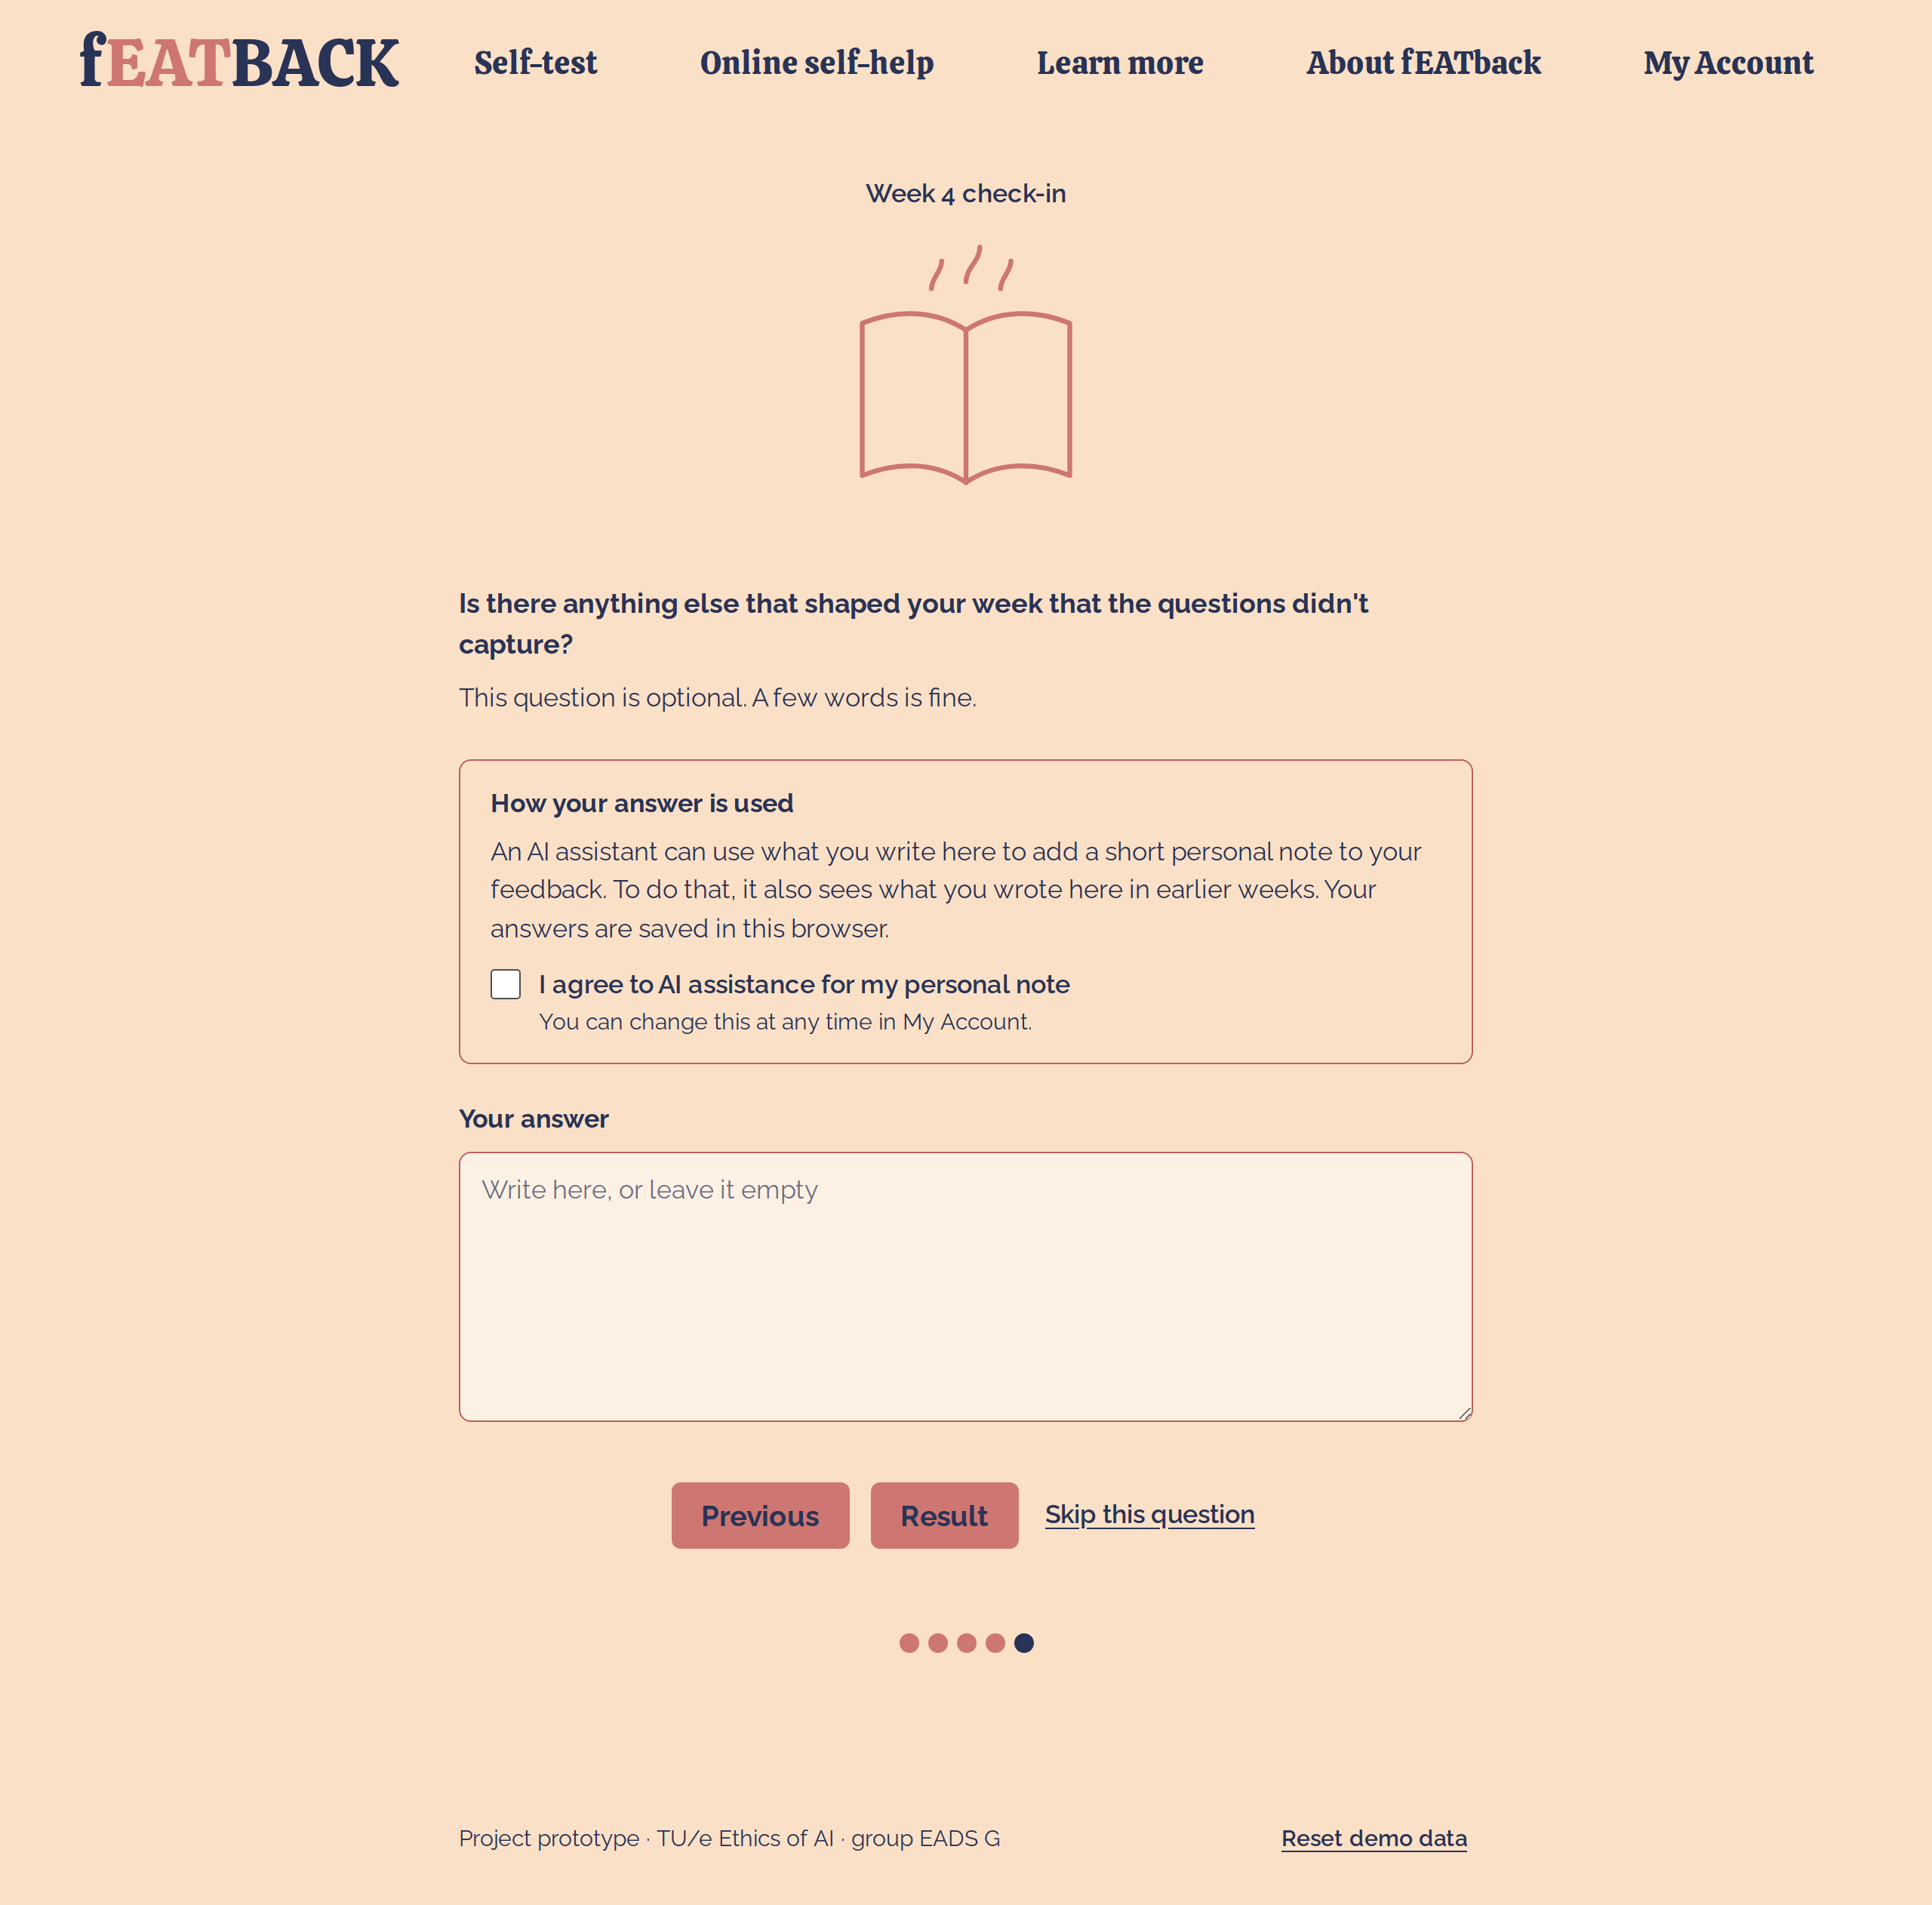
\includegraphics[width=\linewidth, trim=590 1087 590 760, clip]{q5_unticked.png}};
  \begin{scope}[x={(s.south east)}, y={(s.north west)}]
    \callout{0.979}{0.637}{1}
  \end{scope}
\end{tikzpicture}
\par\vspace{4mm}
\paneltitle{b}{Her answer and the result}
\begin{tikzpicture}
  \node[shot] (s) at (0,0) {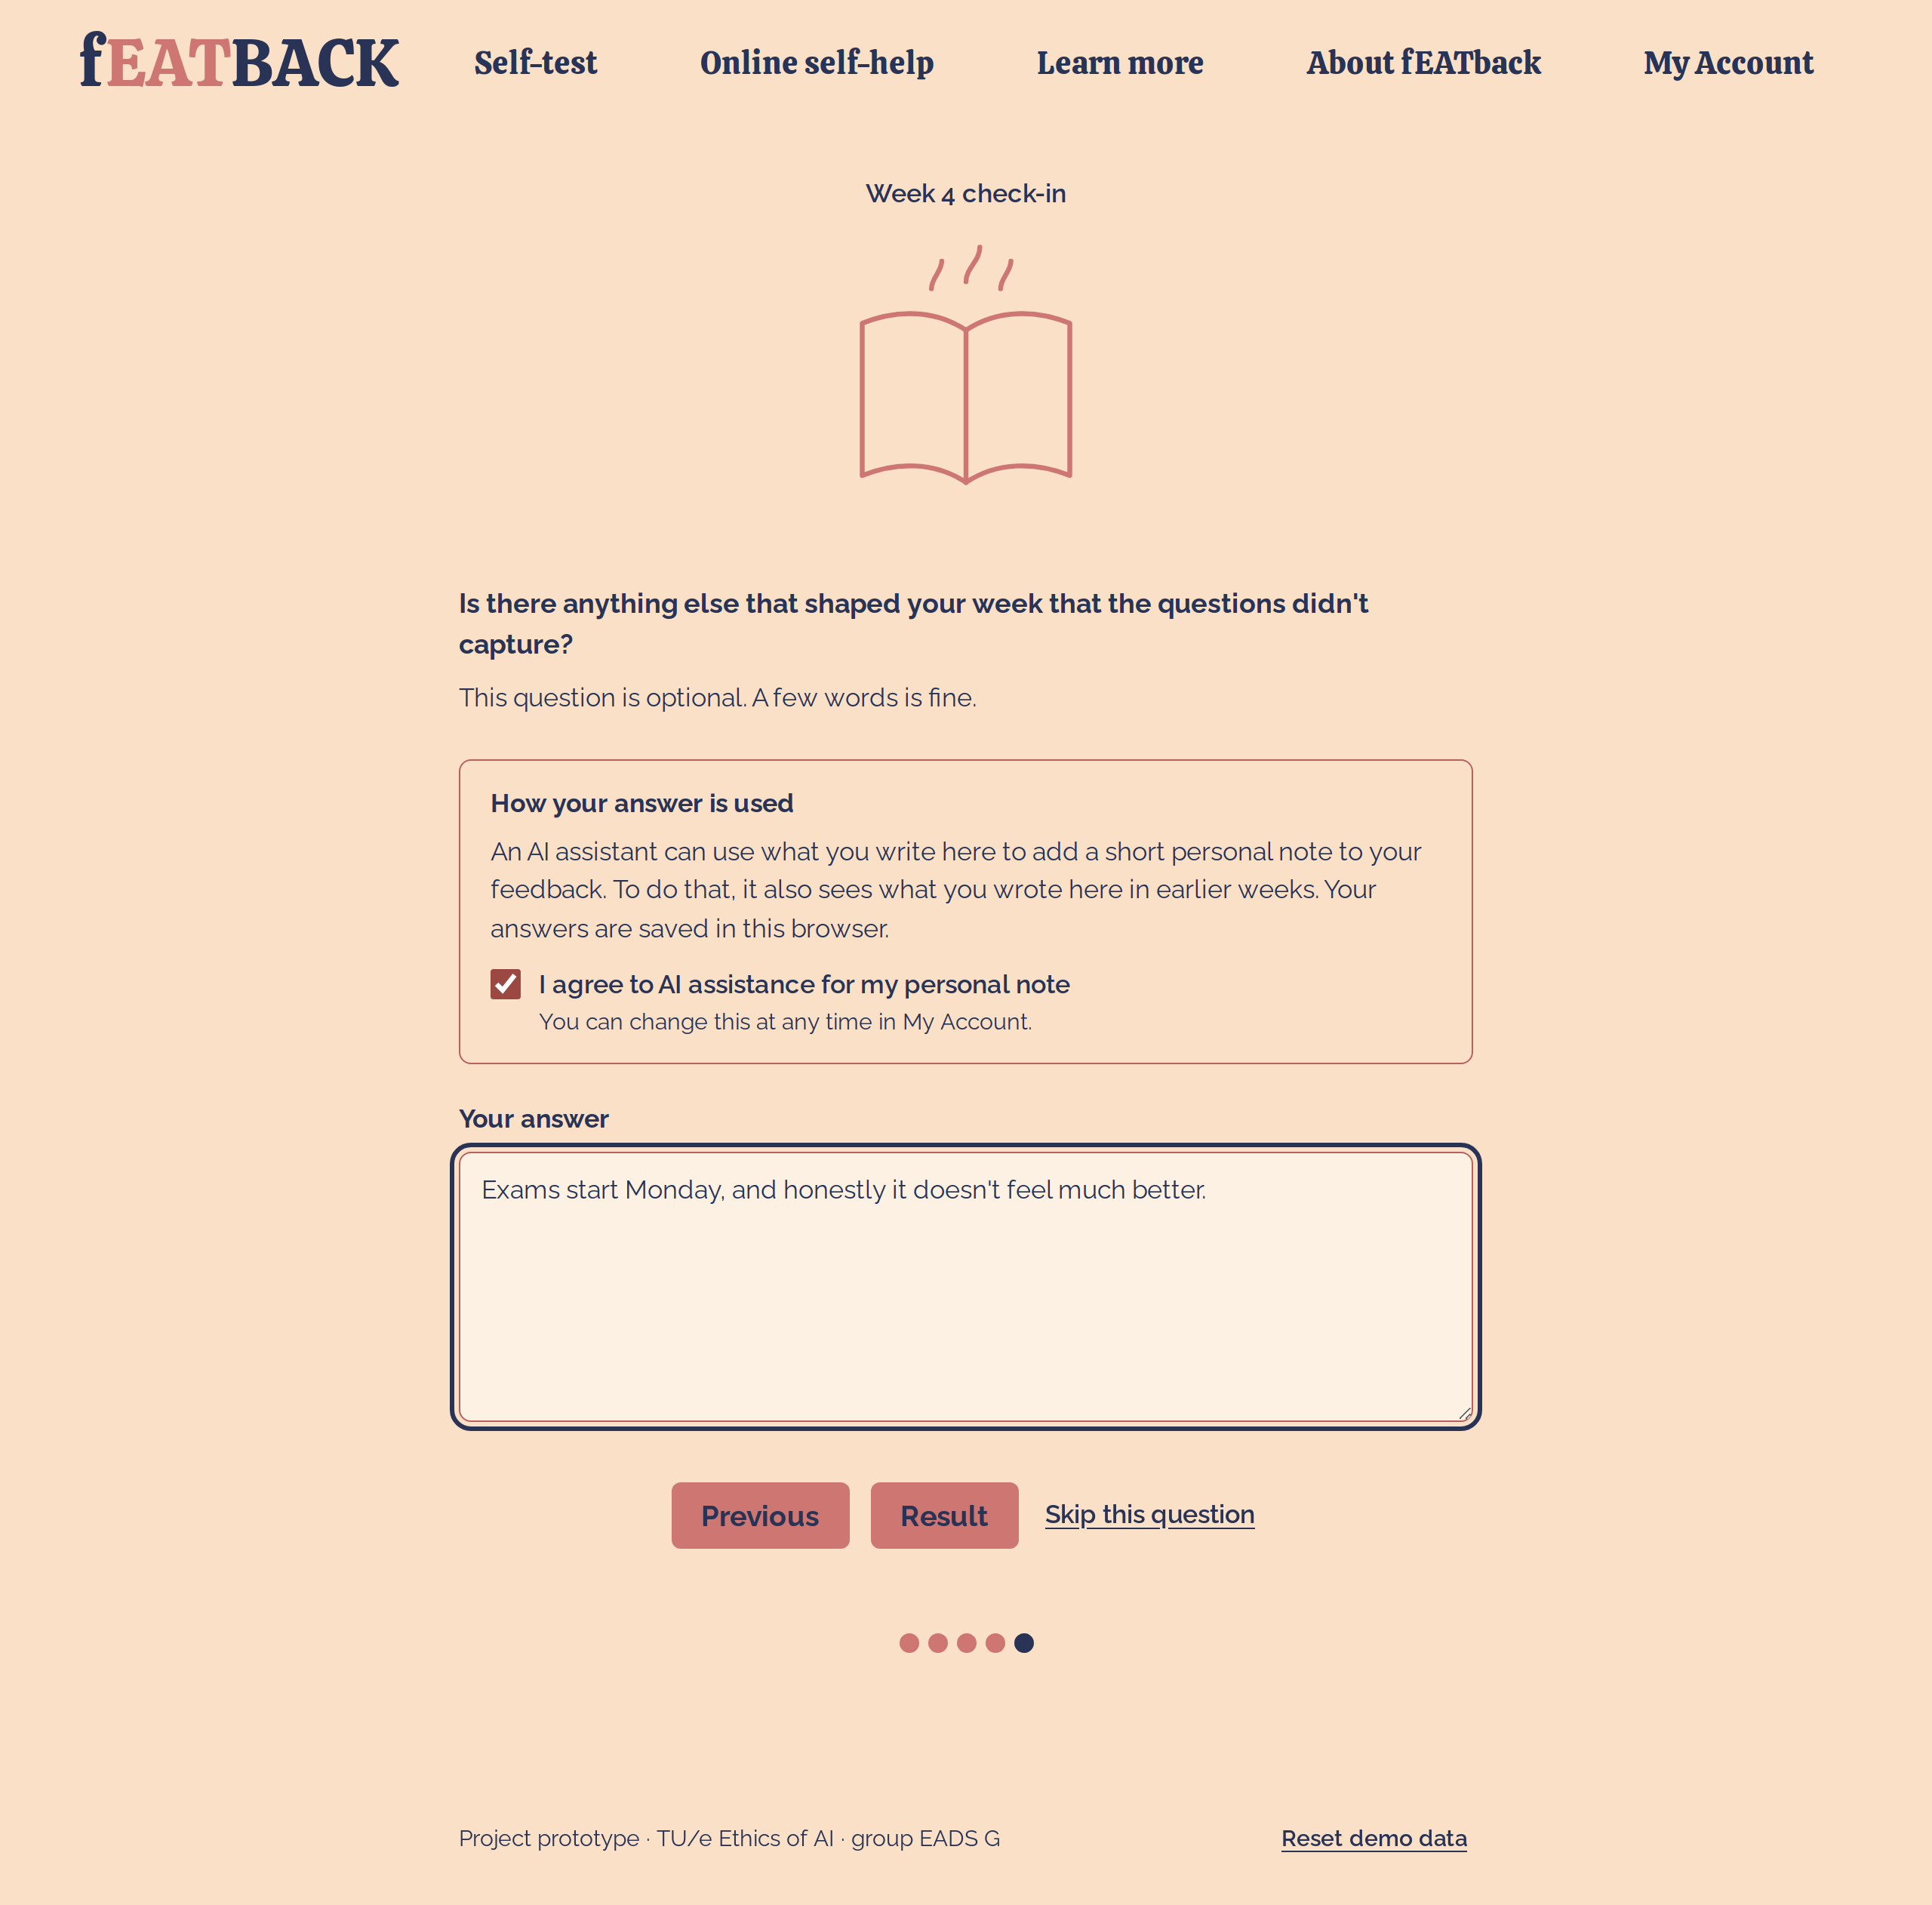
\includegraphics[width=\linewidth, trim=590 613 590 1440, clip]{q5_screen.png}};
  \begin{scope}[x={(s.south east)}, y={(s.north west)}]
    \callout{0.979}{0.817}{2}
  \end{scope}
\end{tikzpicture}
\par\vspace{1.5mm}
\begin{tikzpicture}
  \node[shot] (s) at (0,0) {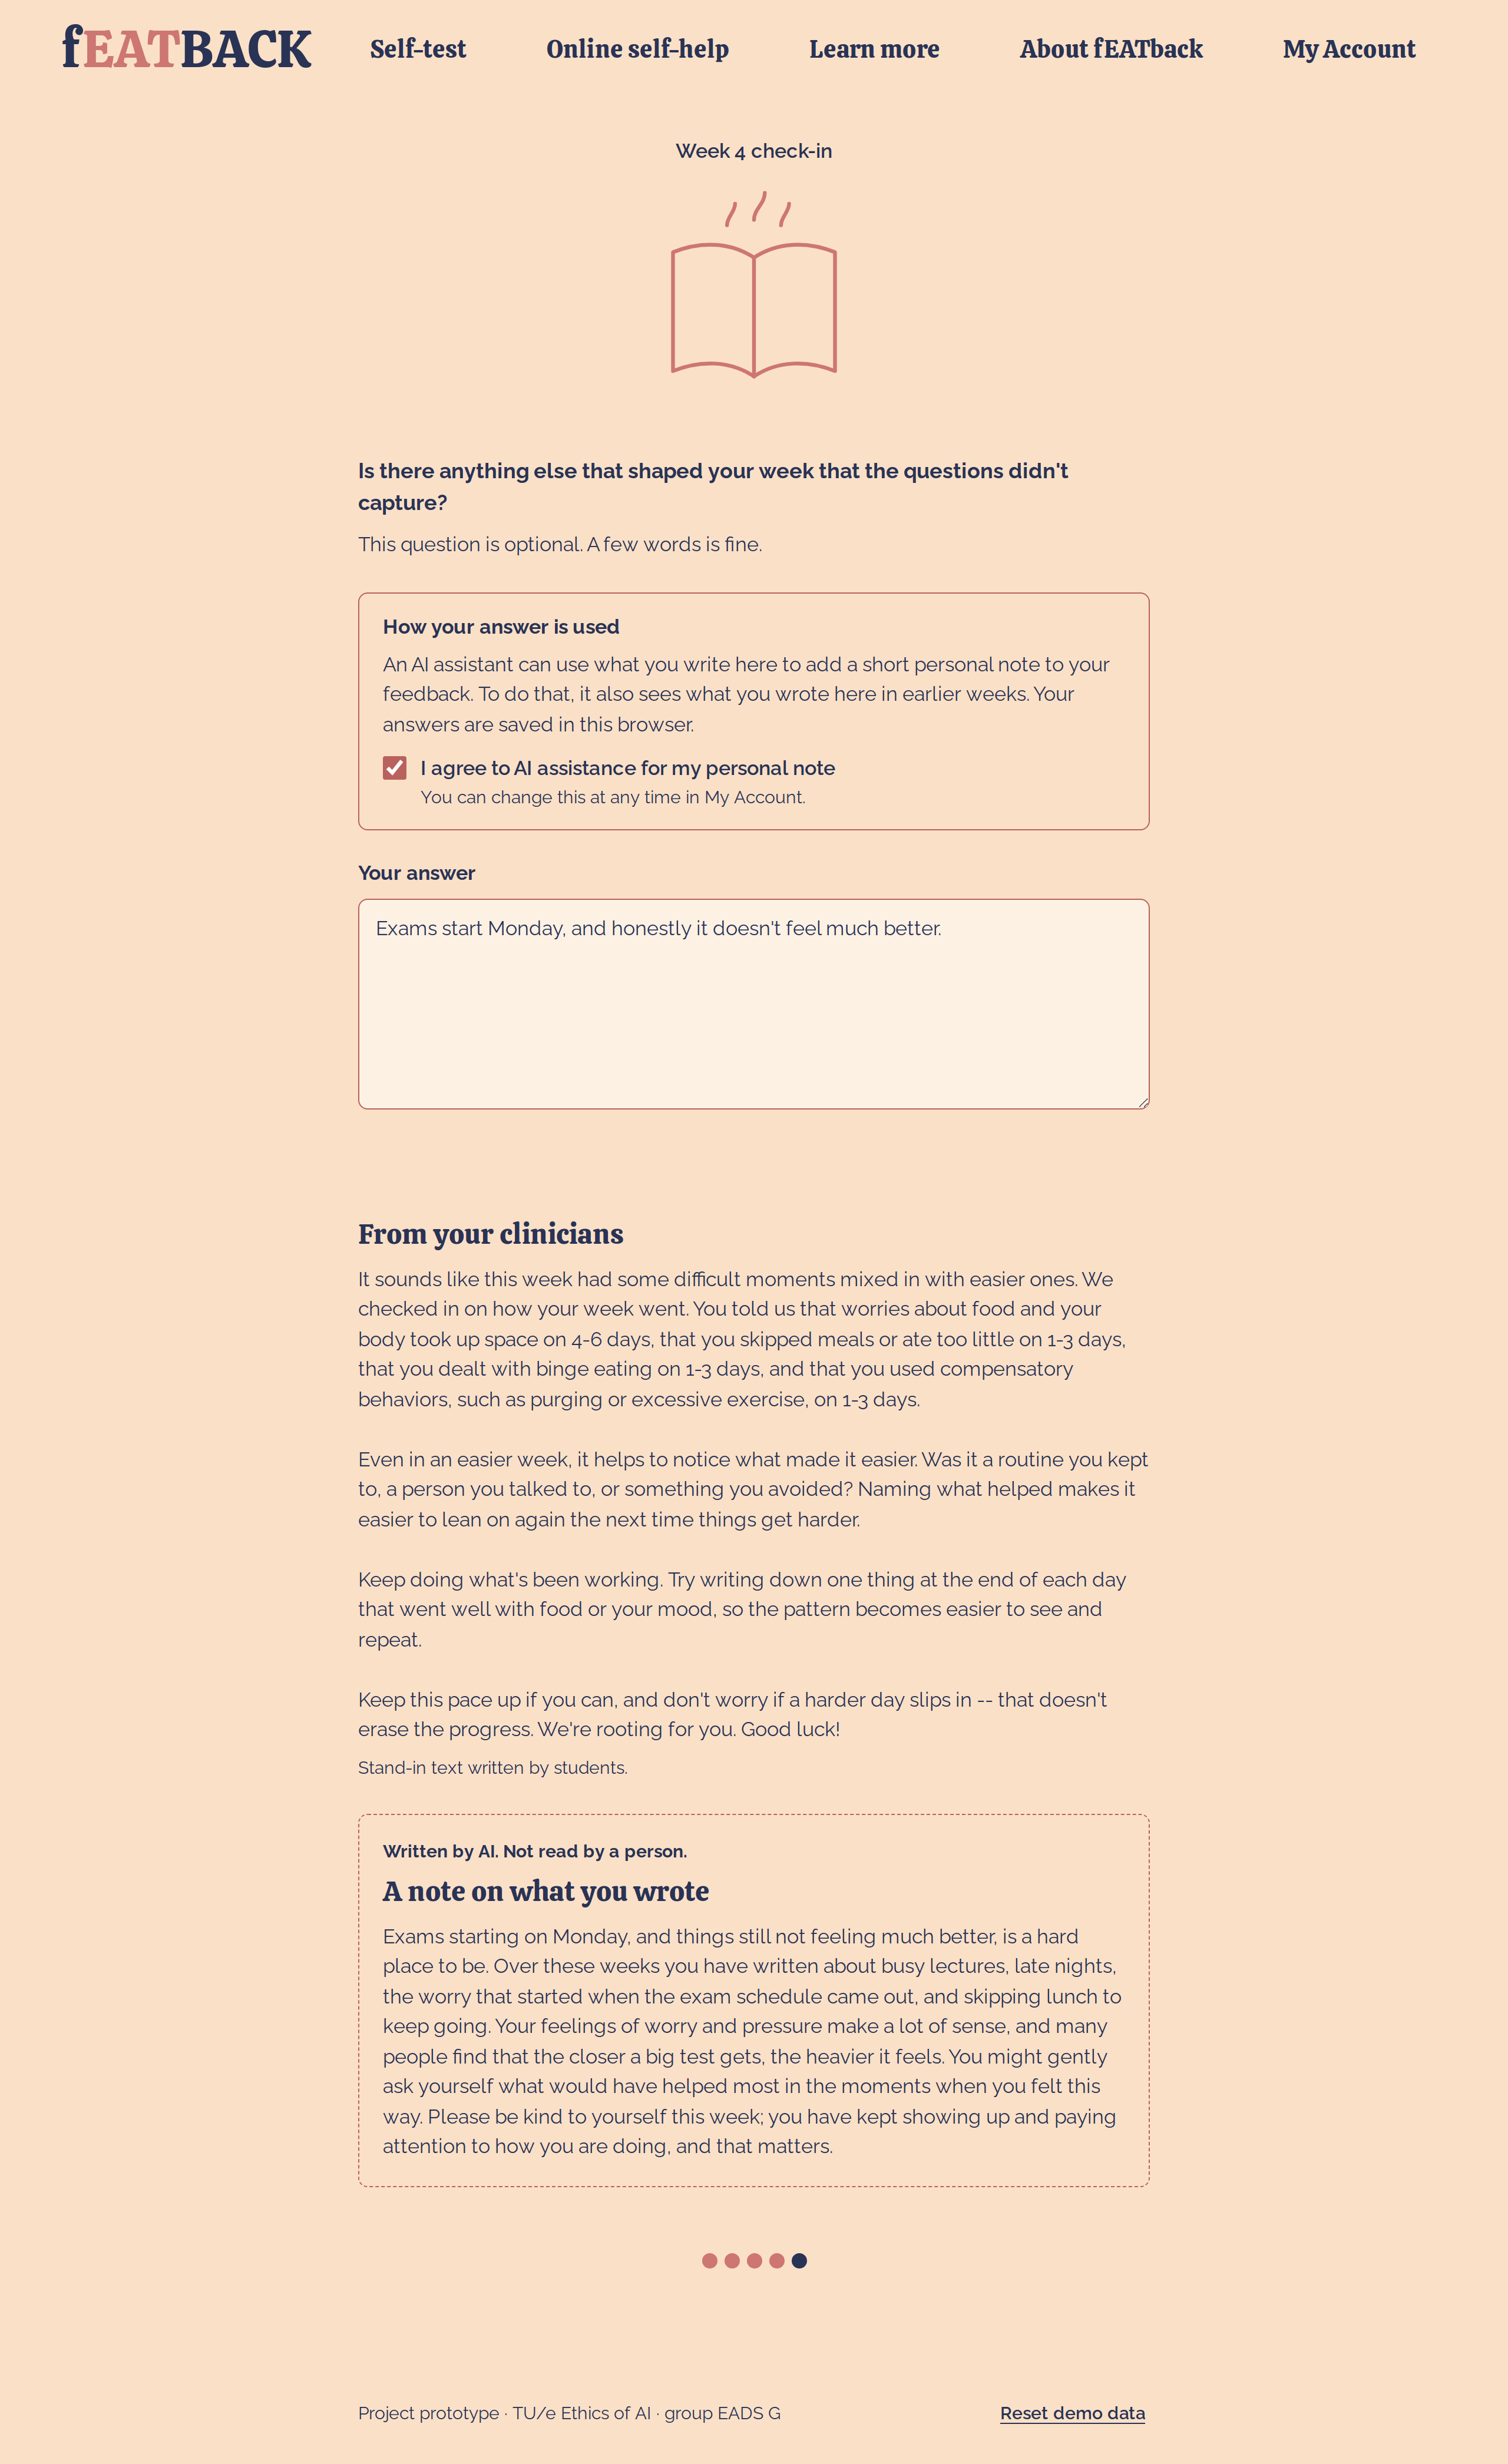
\includegraphics[width=\linewidth, trim=590 443 590 2046, clip]{result_screen.png}};
  \begin{scope}[x={(s.south east)}, y={(s.north west)}]
    \callout{0.979}{0.983}{3}
    \callout{0.979}{0.390}{4}
  \end{scope}
\end{tikzpicture}
\end{minipage}%
\hfill
% ============ Right column: other weeks and edge cases ============
\begin{minipage}[t]{0.47\textwidth}
\colhead{Week 5 and when something goes wrong}
\paneltitle{c}{Week 5, where the note looks back}
\begin{tikzpicture}
  \node[shot] (s) at (0,0) {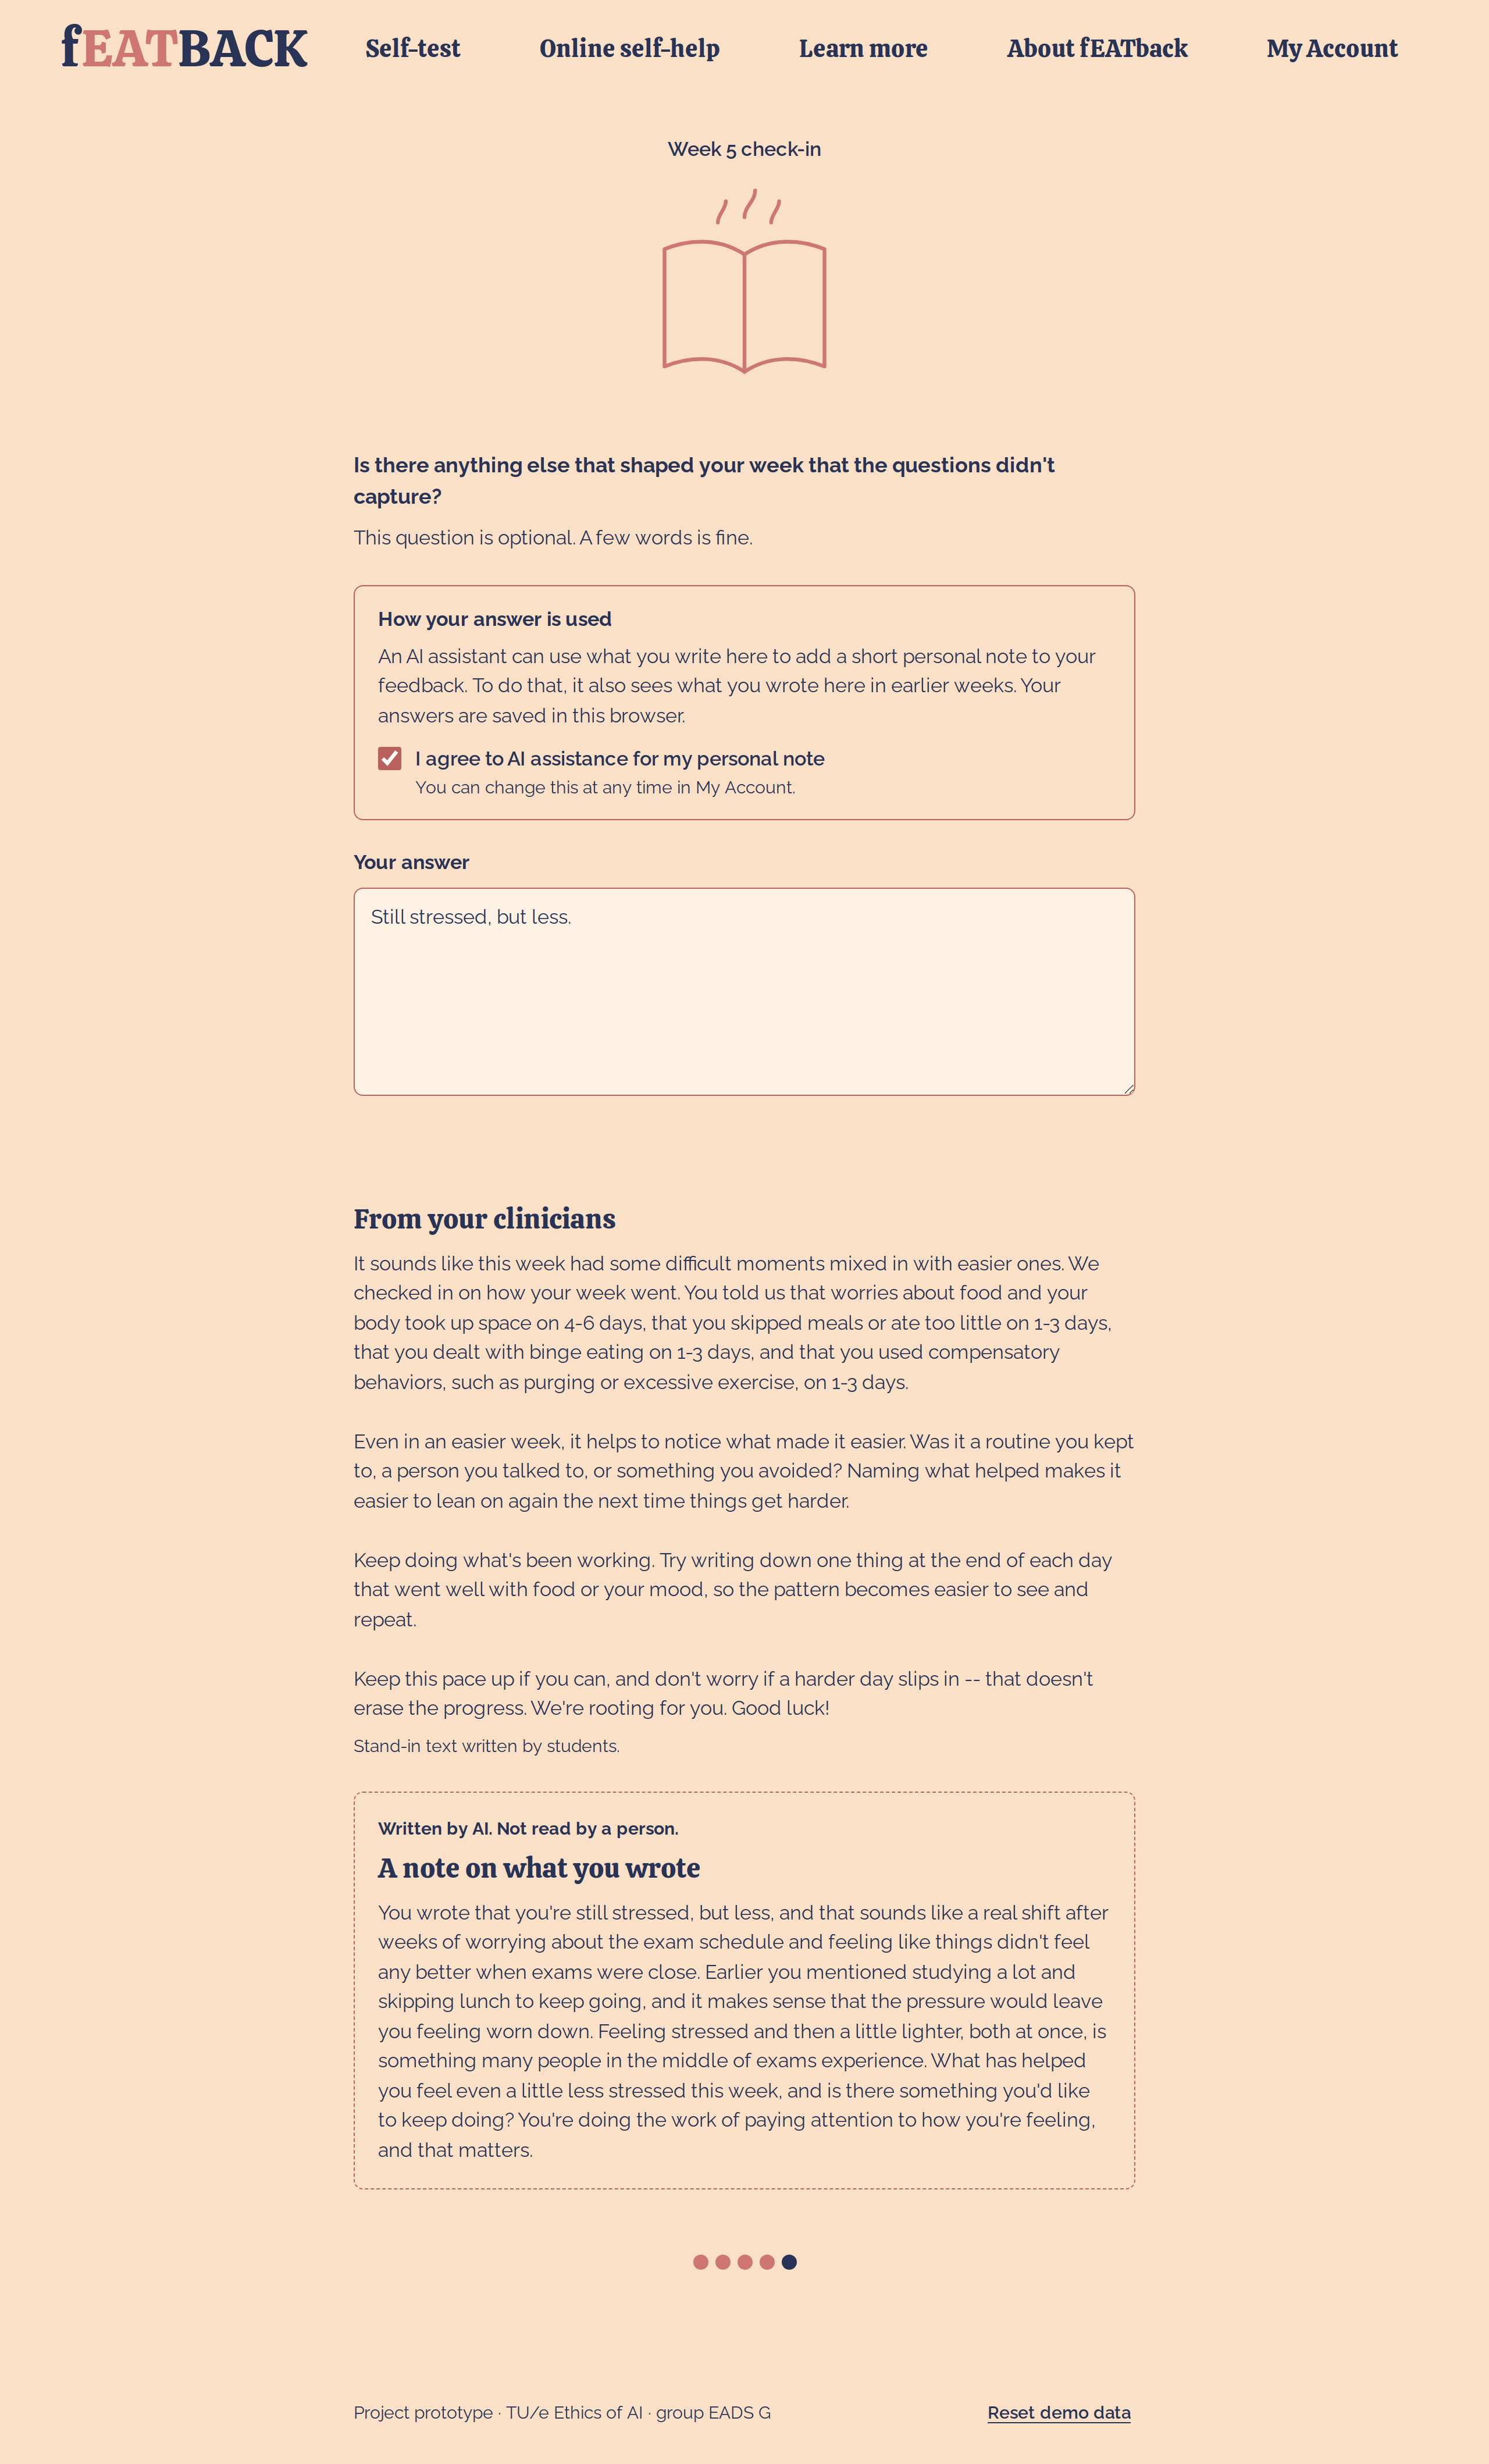
\includegraphics[width=\linewidth, trim=590 2325 590 1440, clip]{result_week5.png}};
\end{tikzpicture}
\par\vspace{1.5mm}
\begin{tikzpicture}
  \node[shot] (s) at (0,0) {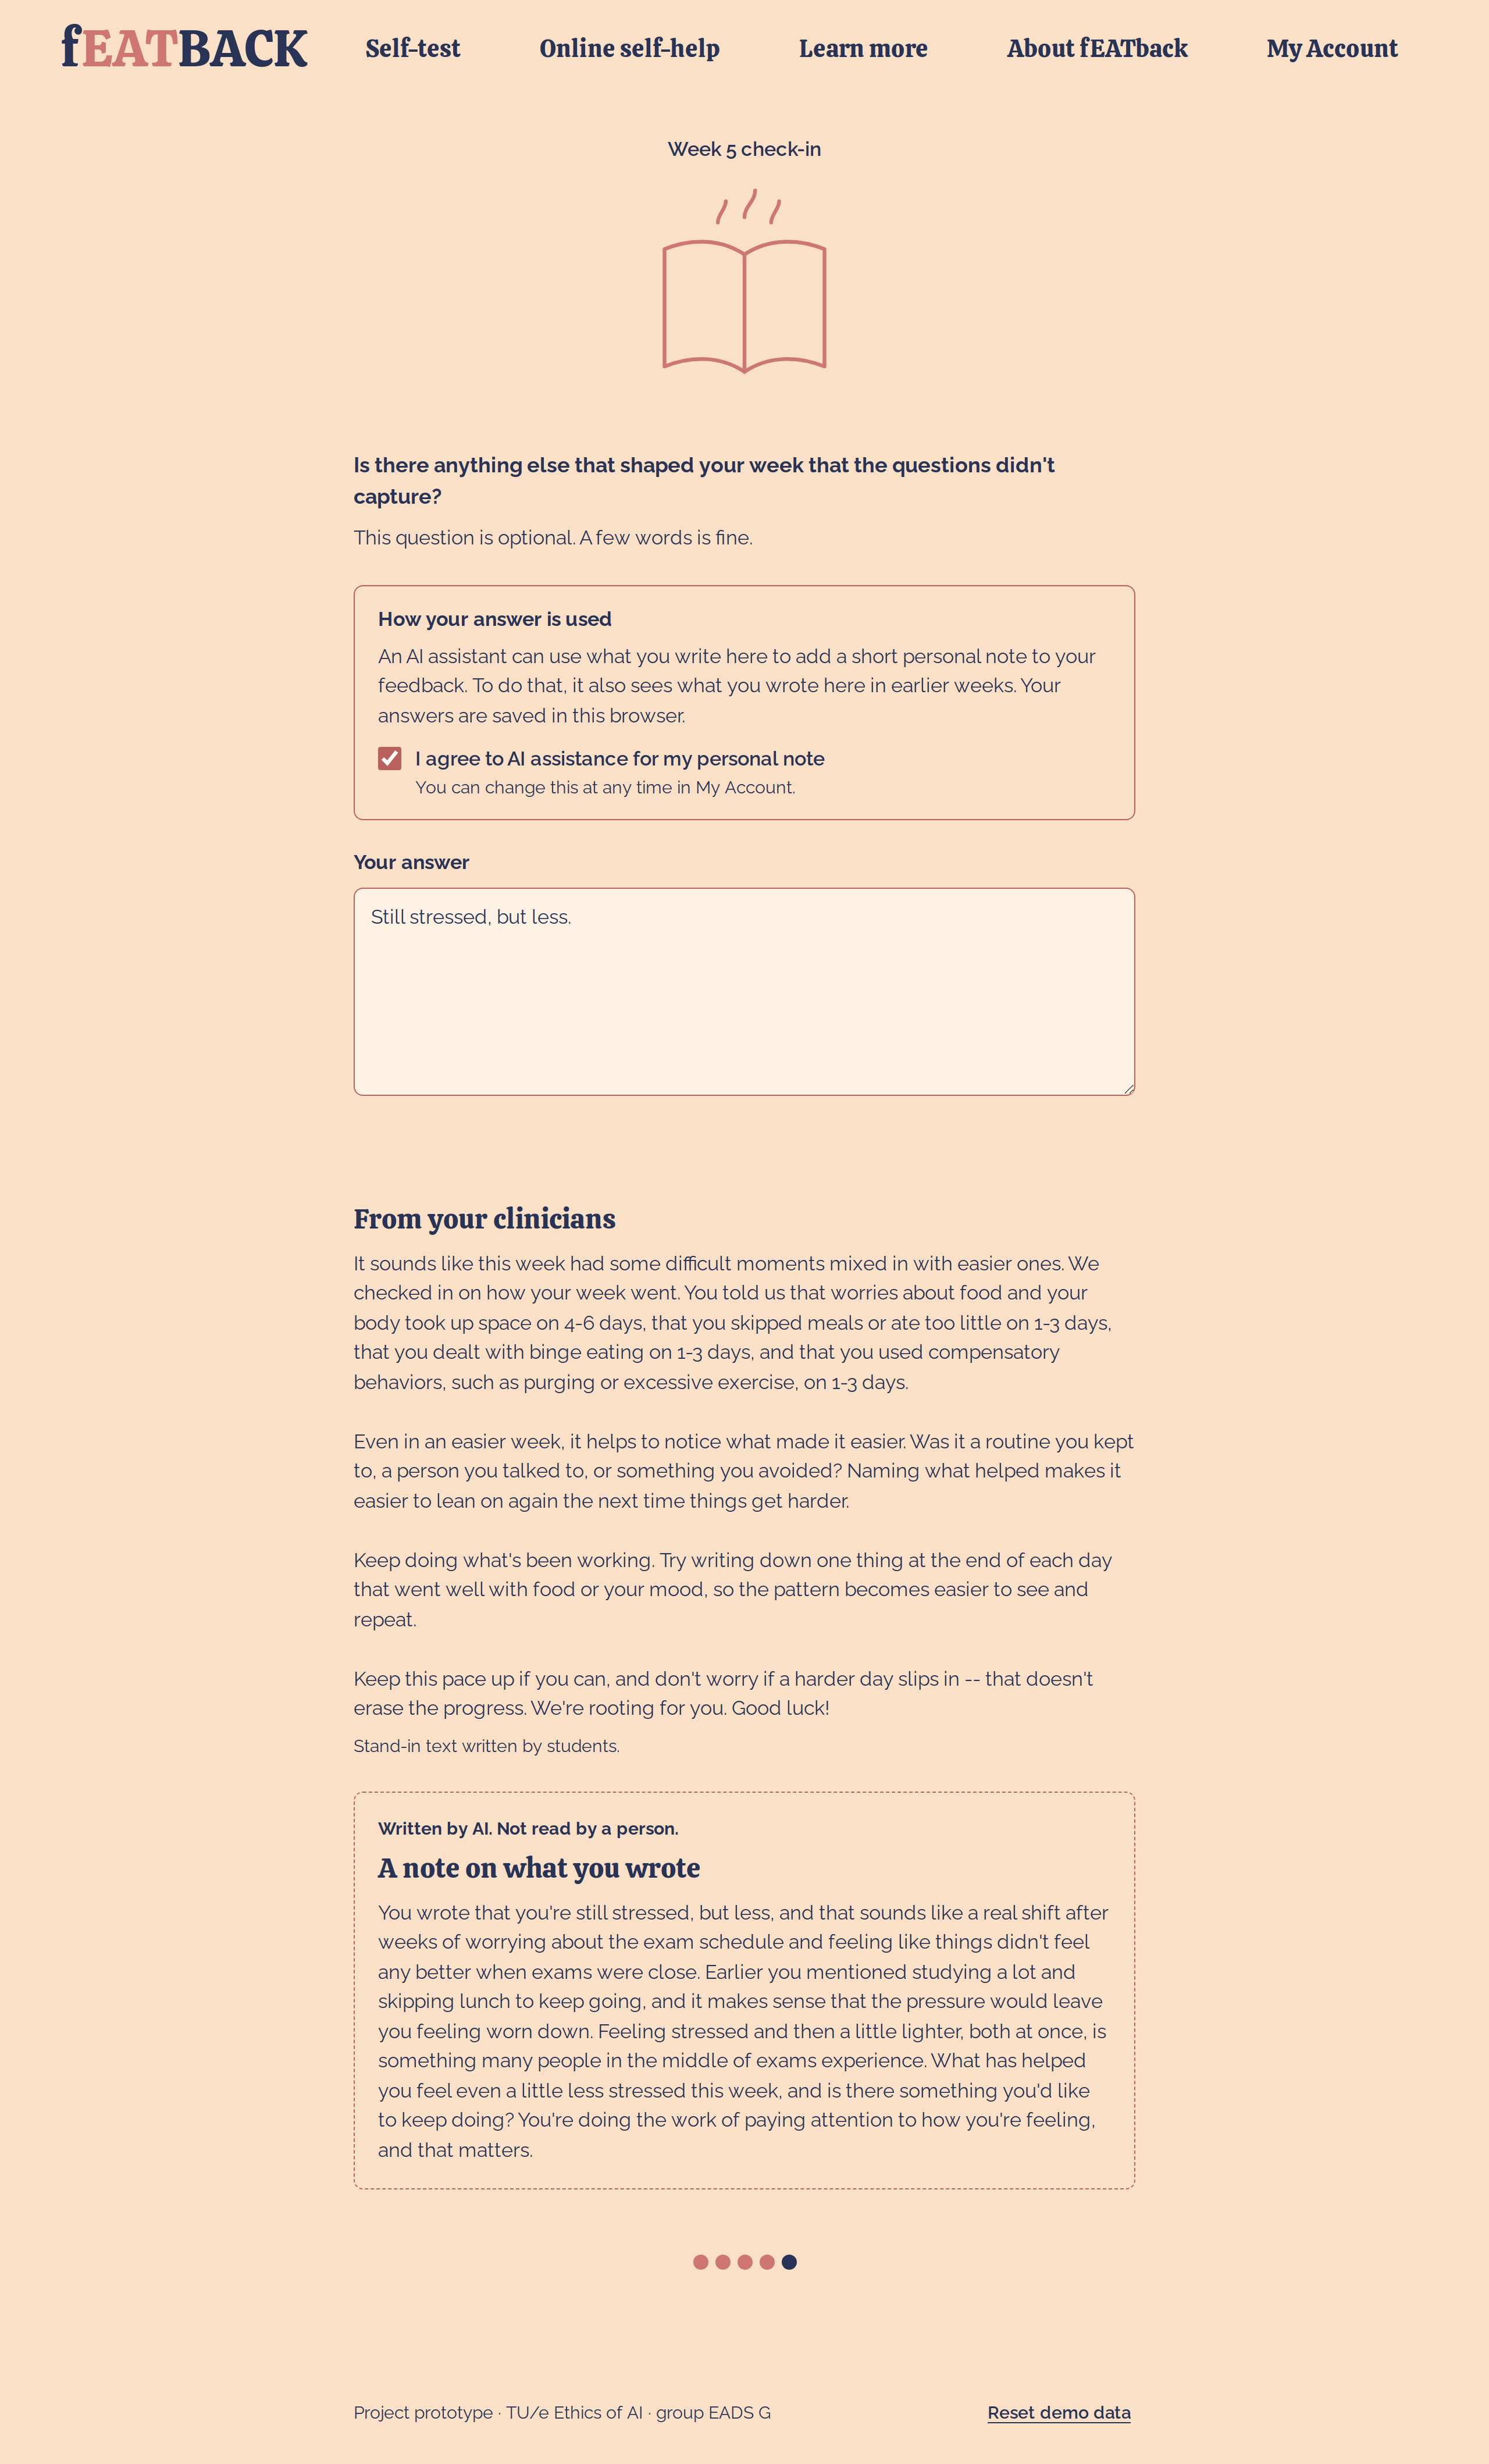
\includegraphics[width=\linewidth, trim=590 445 590 3052, clip]{result_week5.png}};
\end{tikzpicture}
\par\vspace{4mm}
\paneltitle{d}{Model off or note rejected}
\begin{tikzpicture}
  \node[shot] (s) at (0,0) {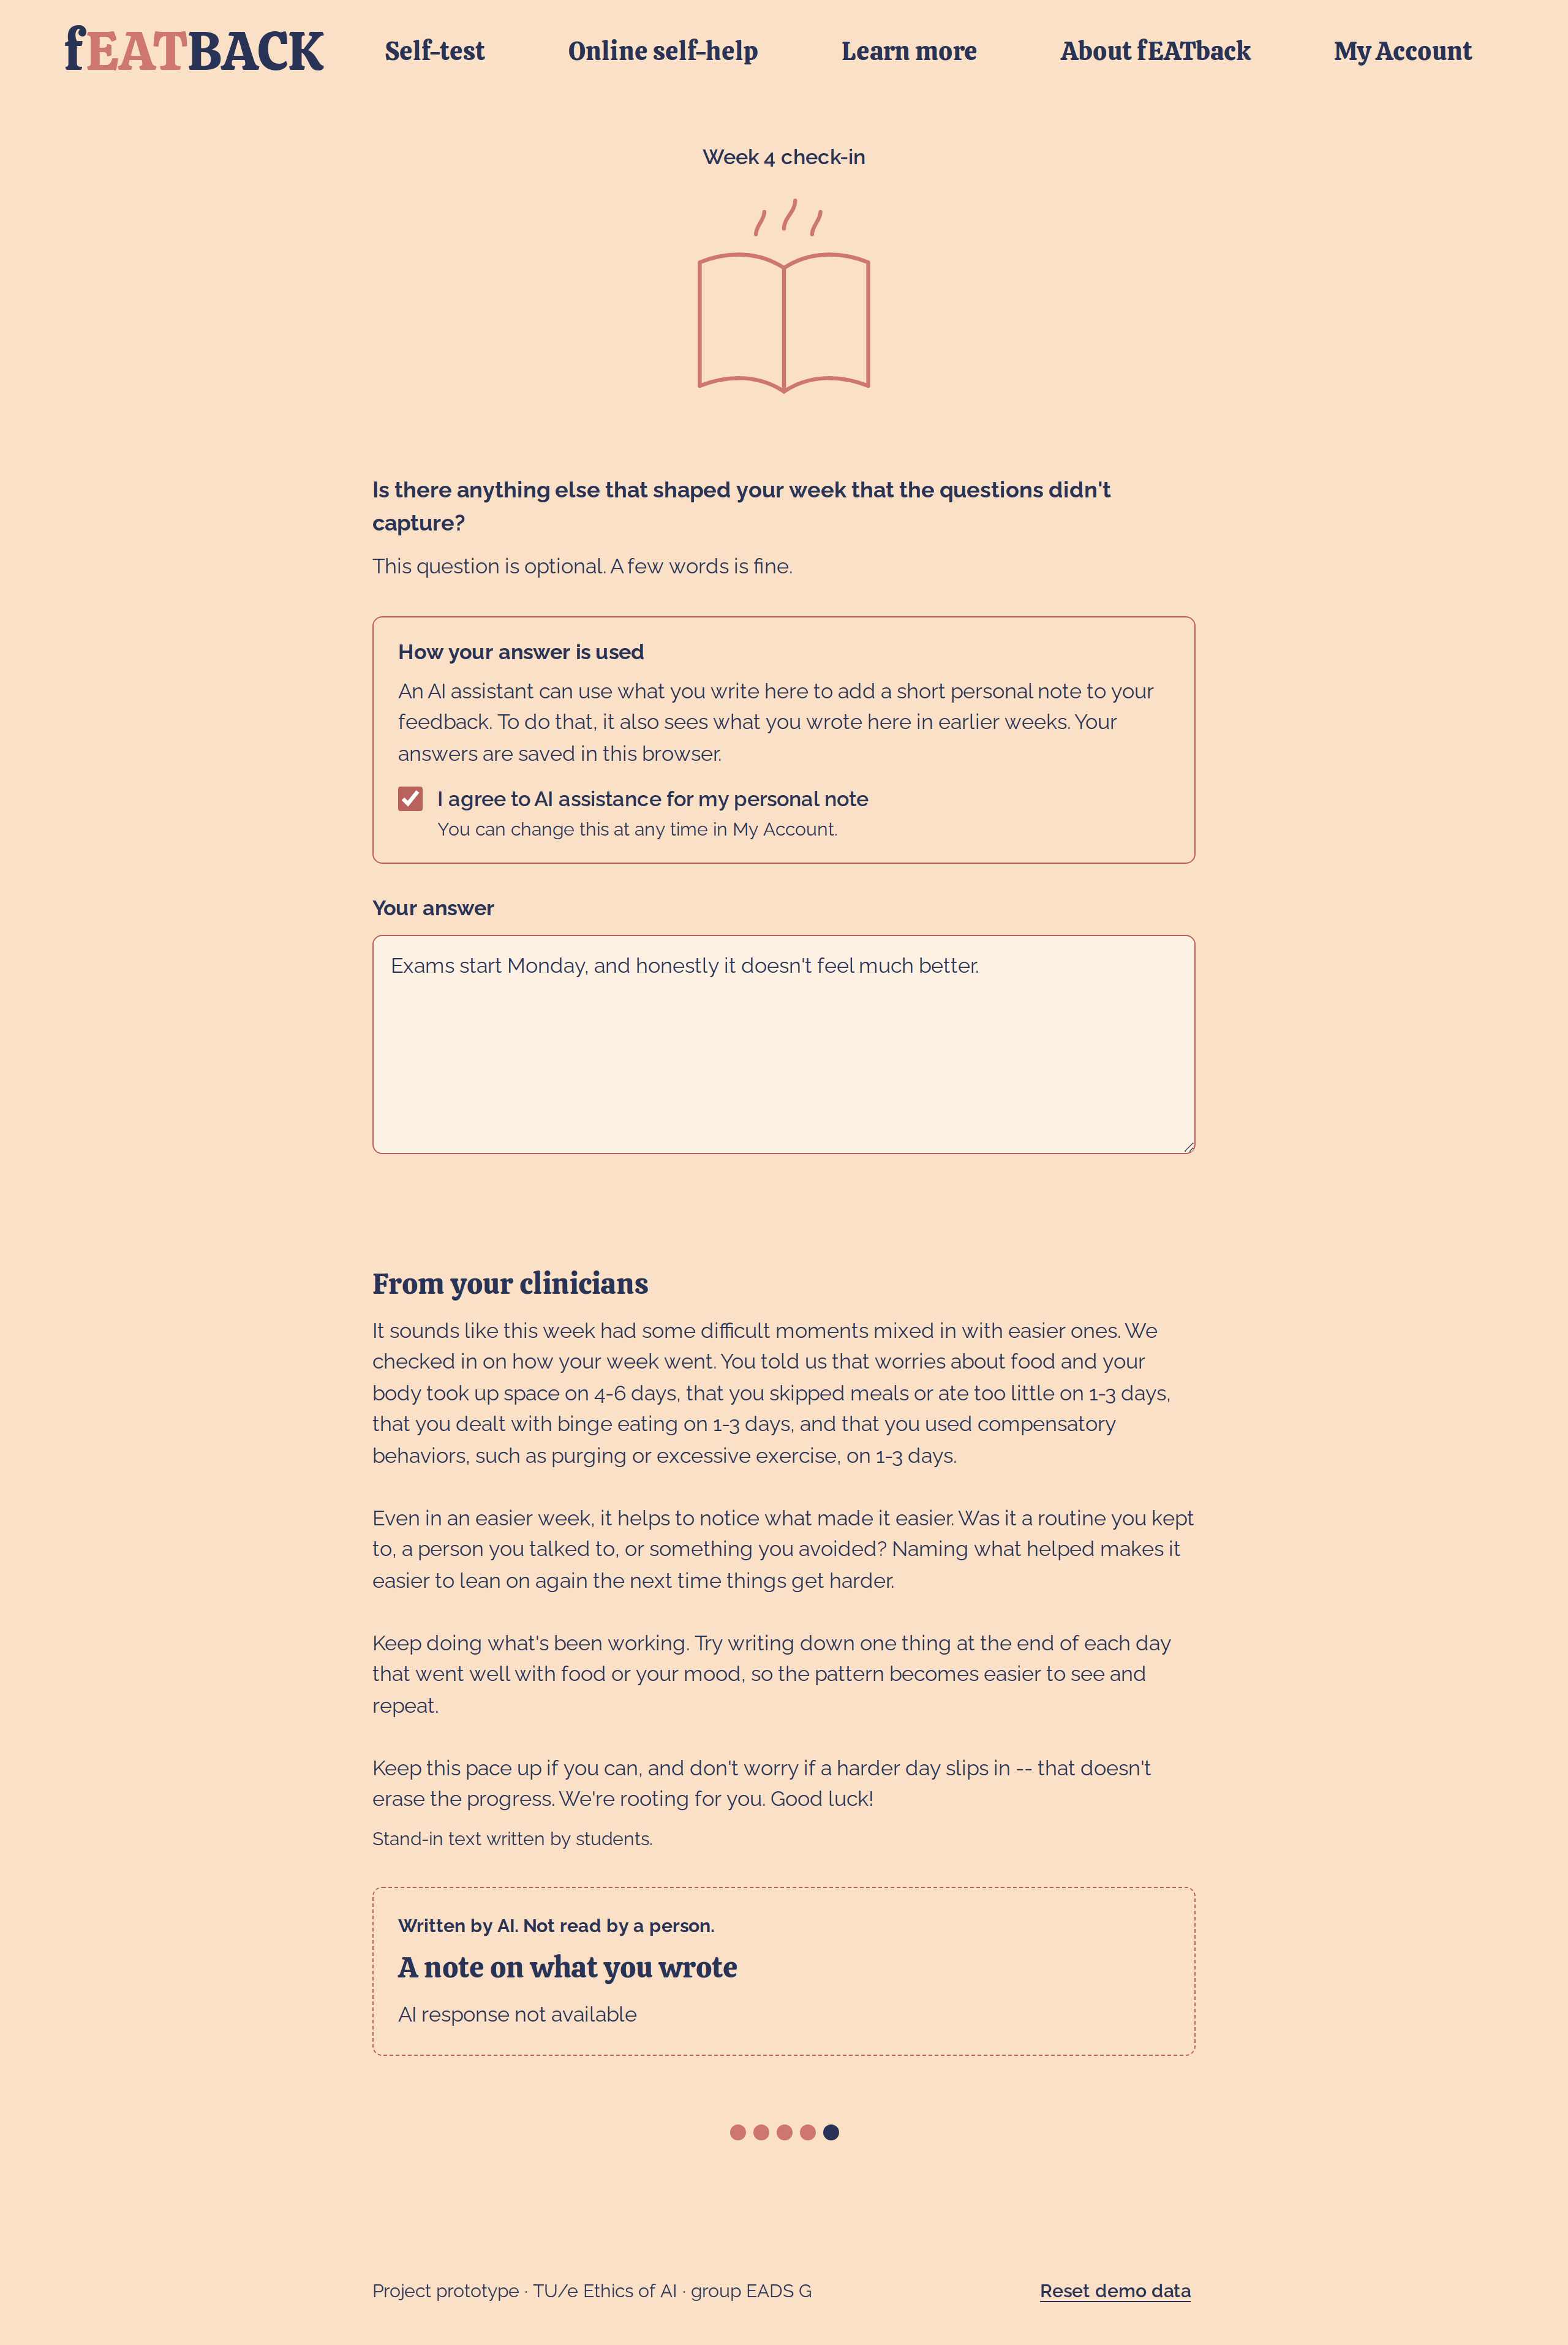
\includegraphics[width=\linewidth, trim=590 445 590 3052, clip]{fallback.png}};
  \begin{scope}[x={(s.south east)}, y={(s.north west)}]
    \callout{0.979}{0.915}{5}
  \end{scope}
\end{tikzpicture}
\par\vspace{4mm}
\paneltitle{e}{An answer with signs of acute risk}
\begin{tikzpicture}
  \node[shot] (s) at (0,0) {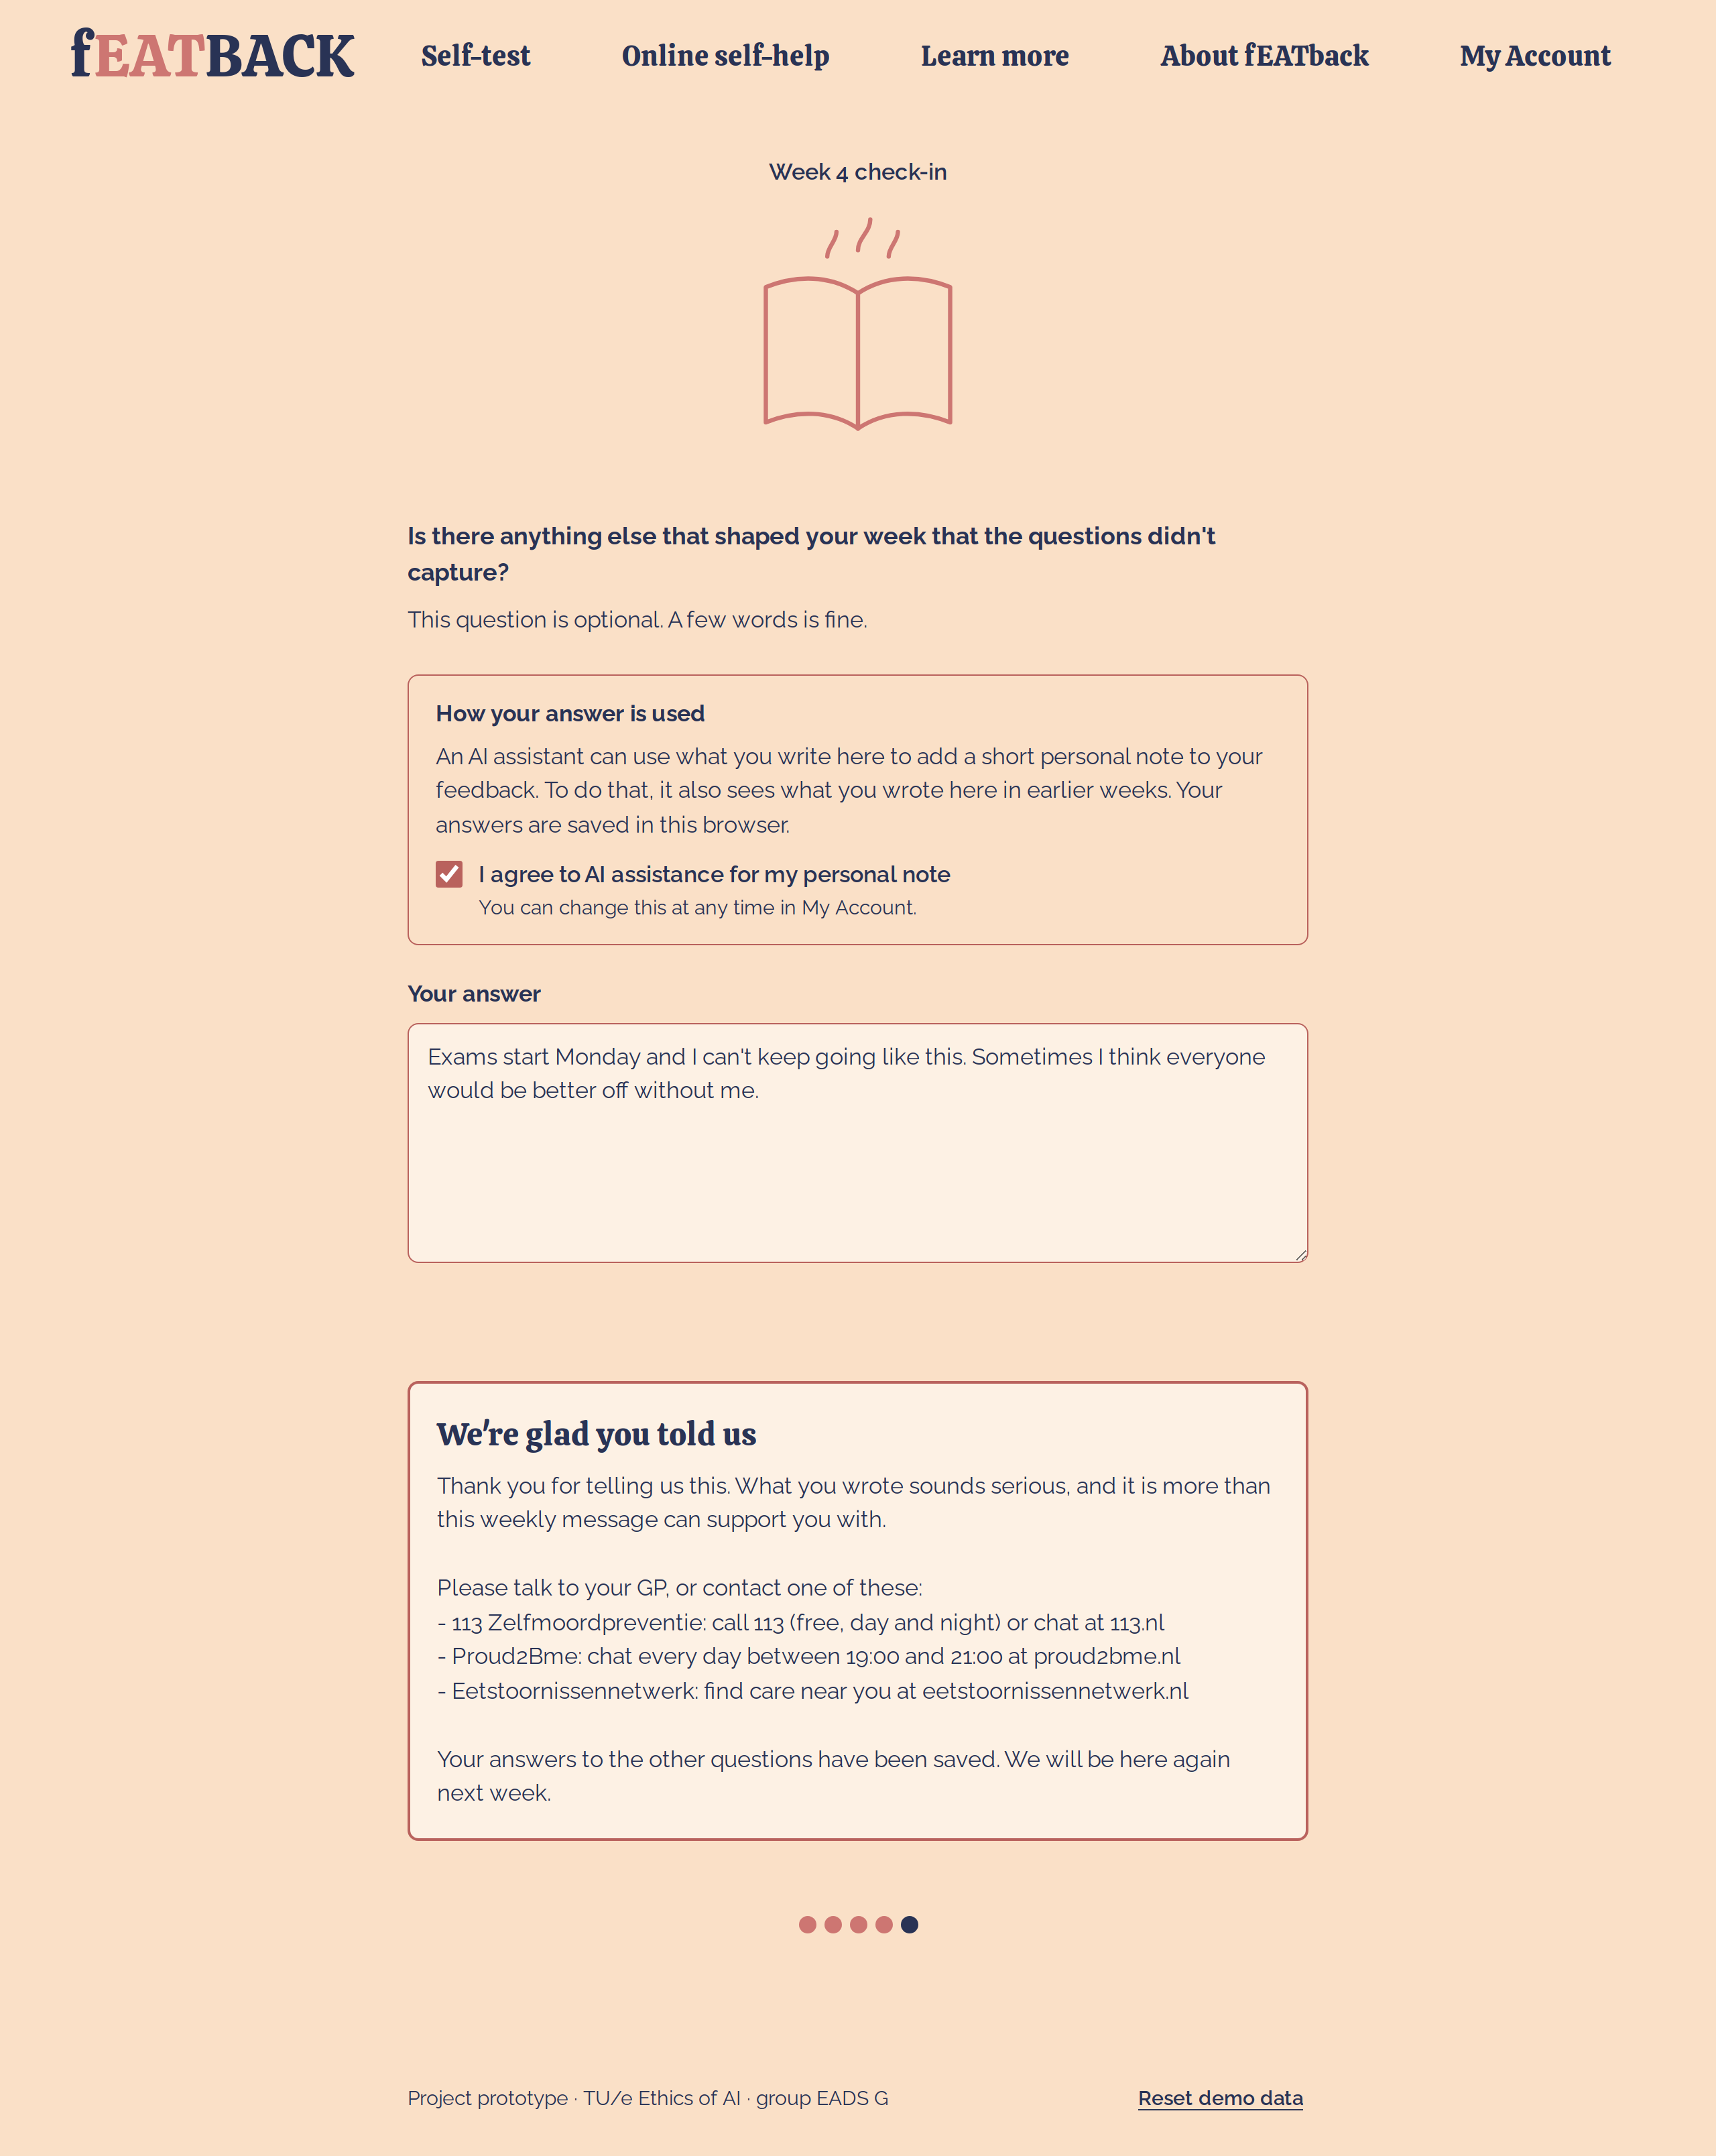
\includegraphics[width=\linewidth, trim=590 1305 590 1440, clip]{acute.png}};
\end{tikzpicture}
\par\vspace{1.5mm}
\begin{tikzpicture}
  \node[shot] (s) at (0,0) {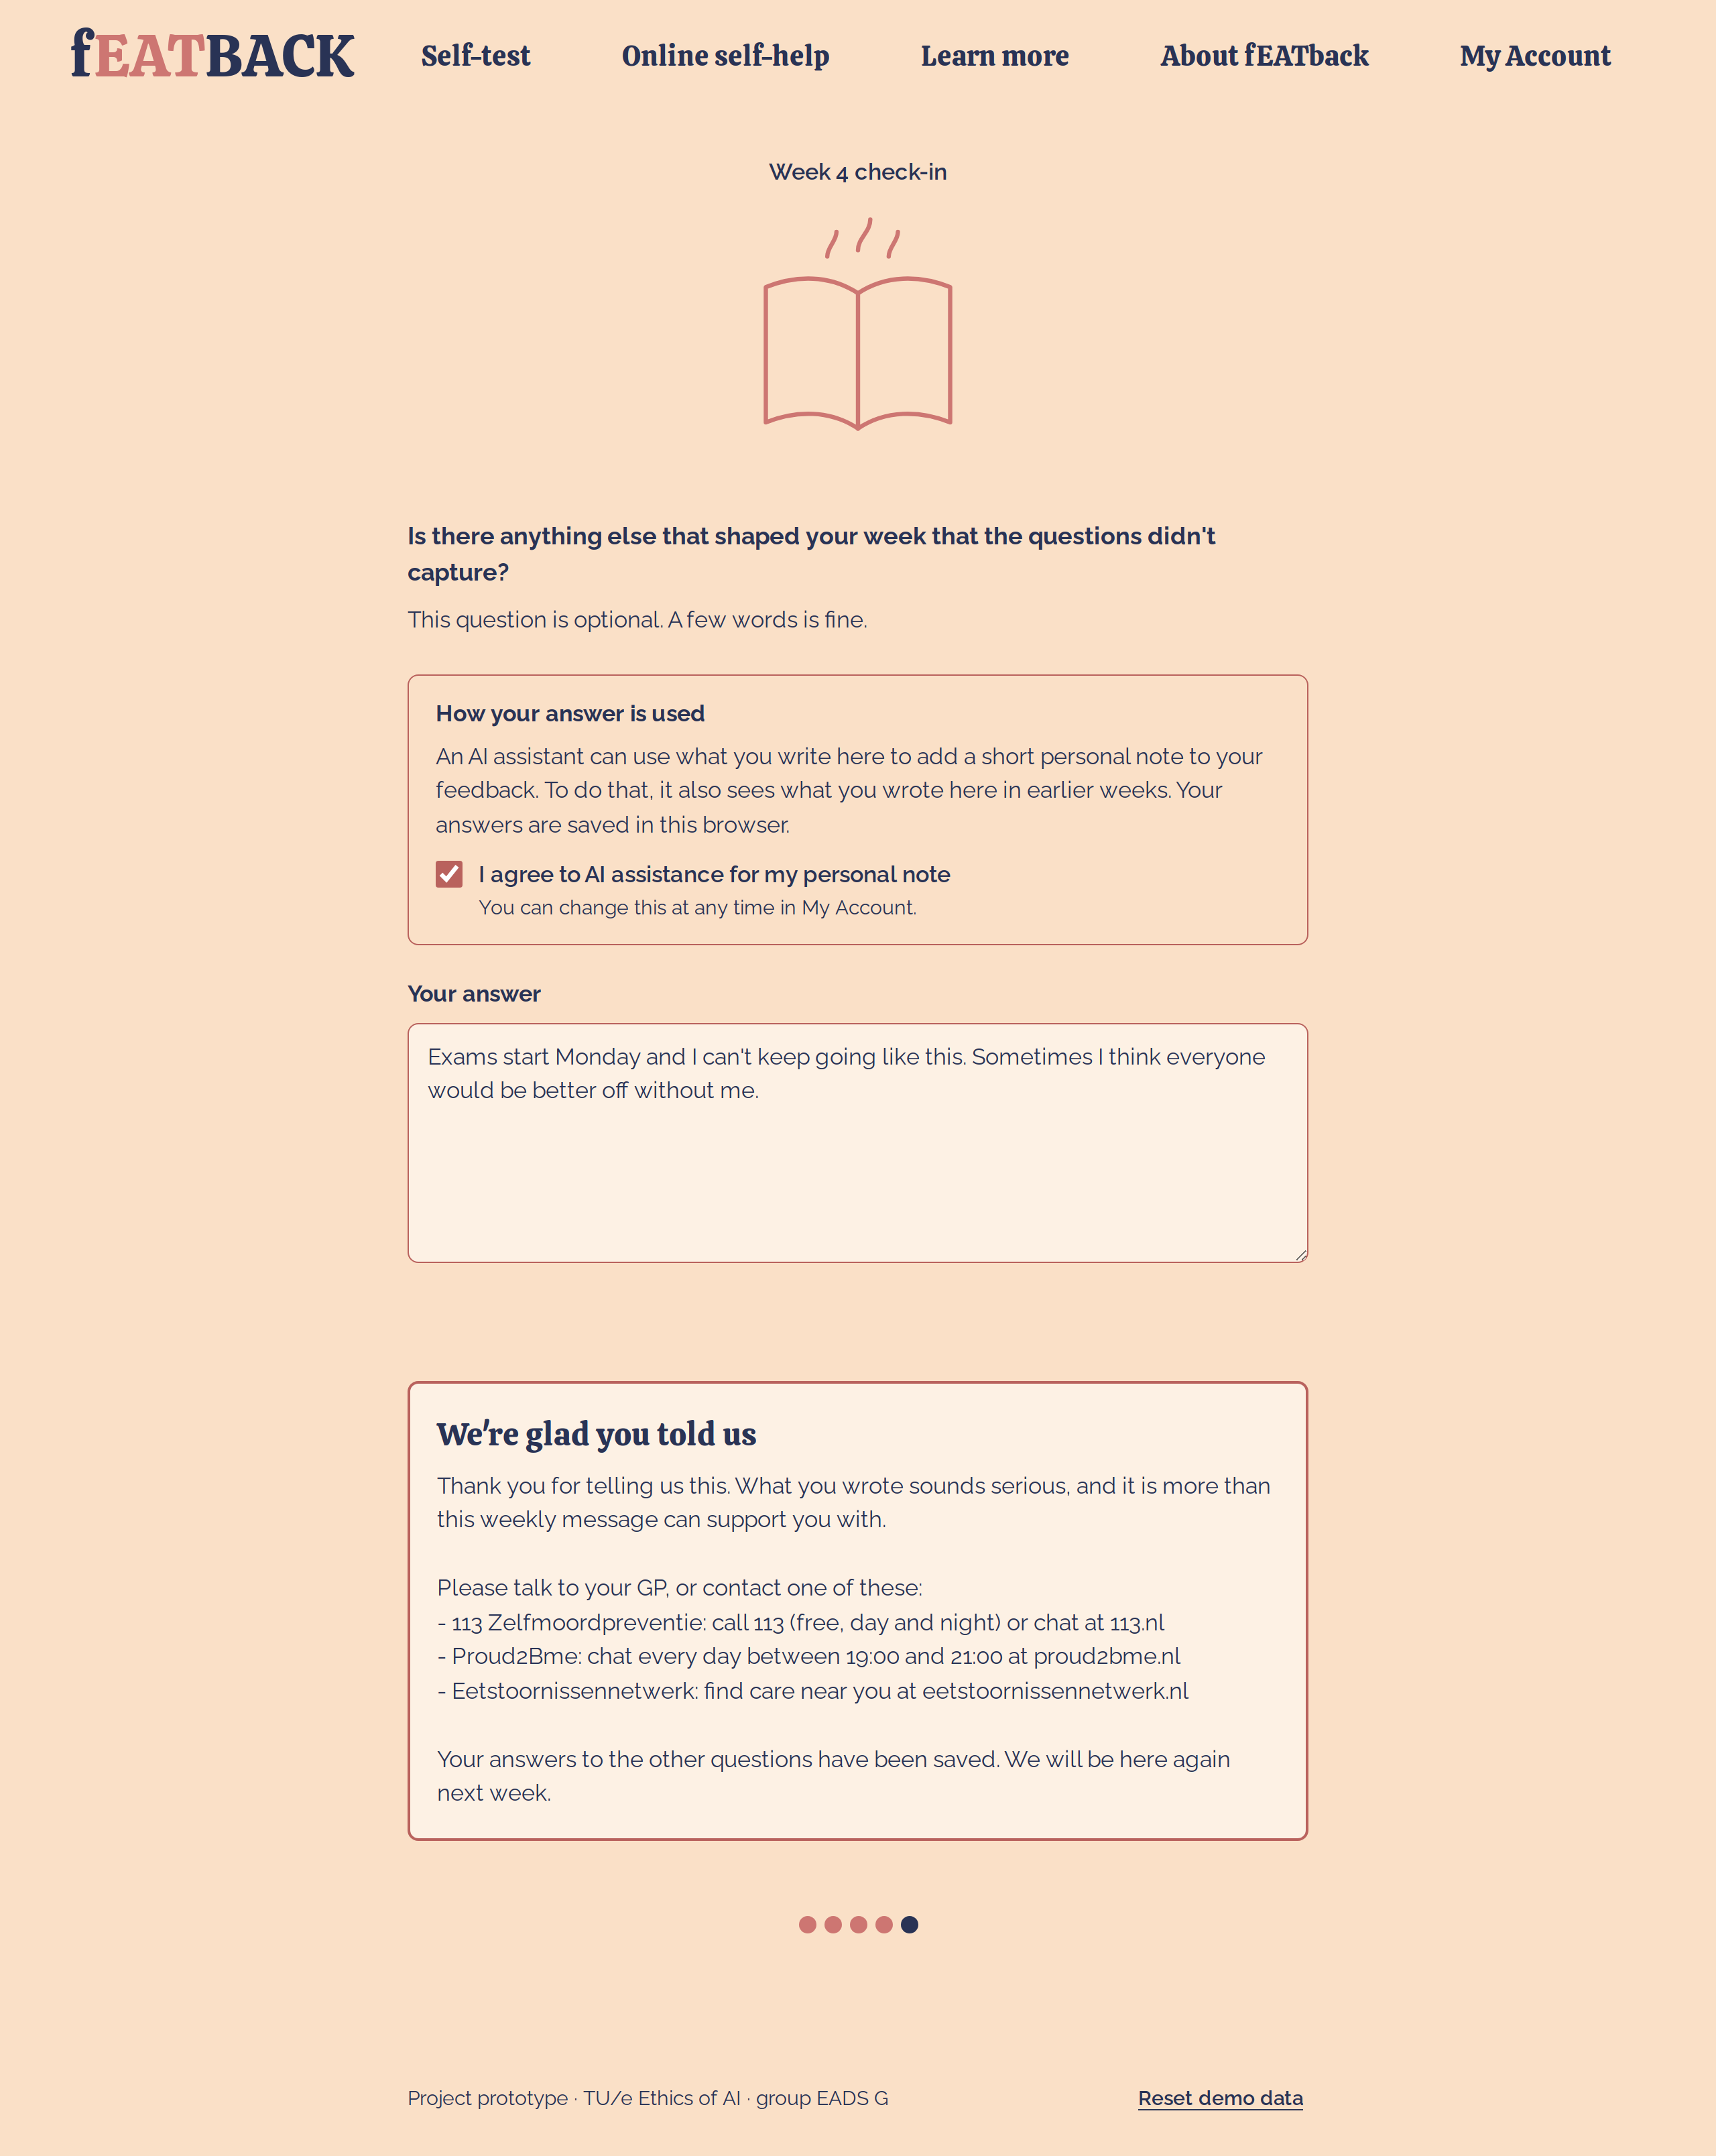
\includegraphics[width=\linewidth, trim=590 443 590 2032, clip]{acute.png}};
  \begin{scope}[x={(s.south east)}, y={(s.north west)}]
    \callout{0.979}{0.962}{6}
  \end{scope}
\end{tikzpicture}
\end{minipage}

\vspace{5mm}
% ---- Key: one entry per callout, aligned with the two columns ----
\newcommand{\keyline}[2]{\key{#1}\hspace{2mm}#2\par\vspace{1.2mm}}
{\footnotesize\sffamily
\begin{minipage}[t]{0.47\textwidth}
\keyline{1}{Consent box starts unticked (part 3)}
\keyline{2}{Answer stored for the trend (part 3)}
\keyline{3}{Stand-in bank message (part 1)}
\end{minipage}\hfill
\begin{minipage}[t]{0.47\textwidth}
\keyline{4}{Label on every AI note (part 2)}
\keyline{5}{Fixed fallback text we wrote (part 1)}
\keyline{6}{Gate takes the more severe label (part 1)}
\end{minipage}}

\vspace{2mm}
\caption{Maren's check-ins from Section~\ref{sec:narrative} as they appear on screen. Part numbers in the key
point to the Responsible Innovation statement. The AI notes in (b) and (c) are real
output from our fine-tuned writer model, run on 12 October 2026. The bank message, Maren
and her earlier answers are made up for the demo.}
\label{fig:mockup}
\end{figure}
.
% Needs tikz (loaded by todonotes in main.tex), graphicx and float.

% ---- Figure style ----------------------------------------------------------
\definecolor{fbnavy}{HTML}{283357}
\tikzset{
  shot/.style={anchor=south west, inner sep=0, draw=black!18, line width=0.4pt},
  callout/.style={circle, fill=fbnavy, draw=white, line width=0.9pt, text=white,
    font=\sffamily\bfseries\scriptsize, inner sep=0pt, minimum size=4.4mm}}
% Callouts always sit on the top-right corner of the card they mark.
\newcommand{\callout}[3]{\node[callout, overlay] at (#1,#2) {#3};}
% Inline callout for the key
\newcommand{\key}[1]{\tikz[baseline=-0.6ex]\node[callout]{#1};}
% Panel title
\newcommand{\paneltitle}[2]{{\sffamily\footnotesize\color{fbnavy}\textbf{(#1)}~#2}\par\vspace{1mm}}
\newcommand{\colhead}[1]{{\sffamily\small\bfseries\color{fbnavy}#1}\par\vspace{0.5mm}{\color{black!25}\hrule height 0.4pt}\vspace{2mm}}

\begin{figure}[H]
\centering
% ============ Left column: week 4, the usual path ============
\begin{minipage}[t]{0.47\textwidth}
\colhead{Week 4}
\paneltitle{a}{Question 5, before she agrees}
\begin{tikzpicture}
  \node[shot] (s) at (0,0) {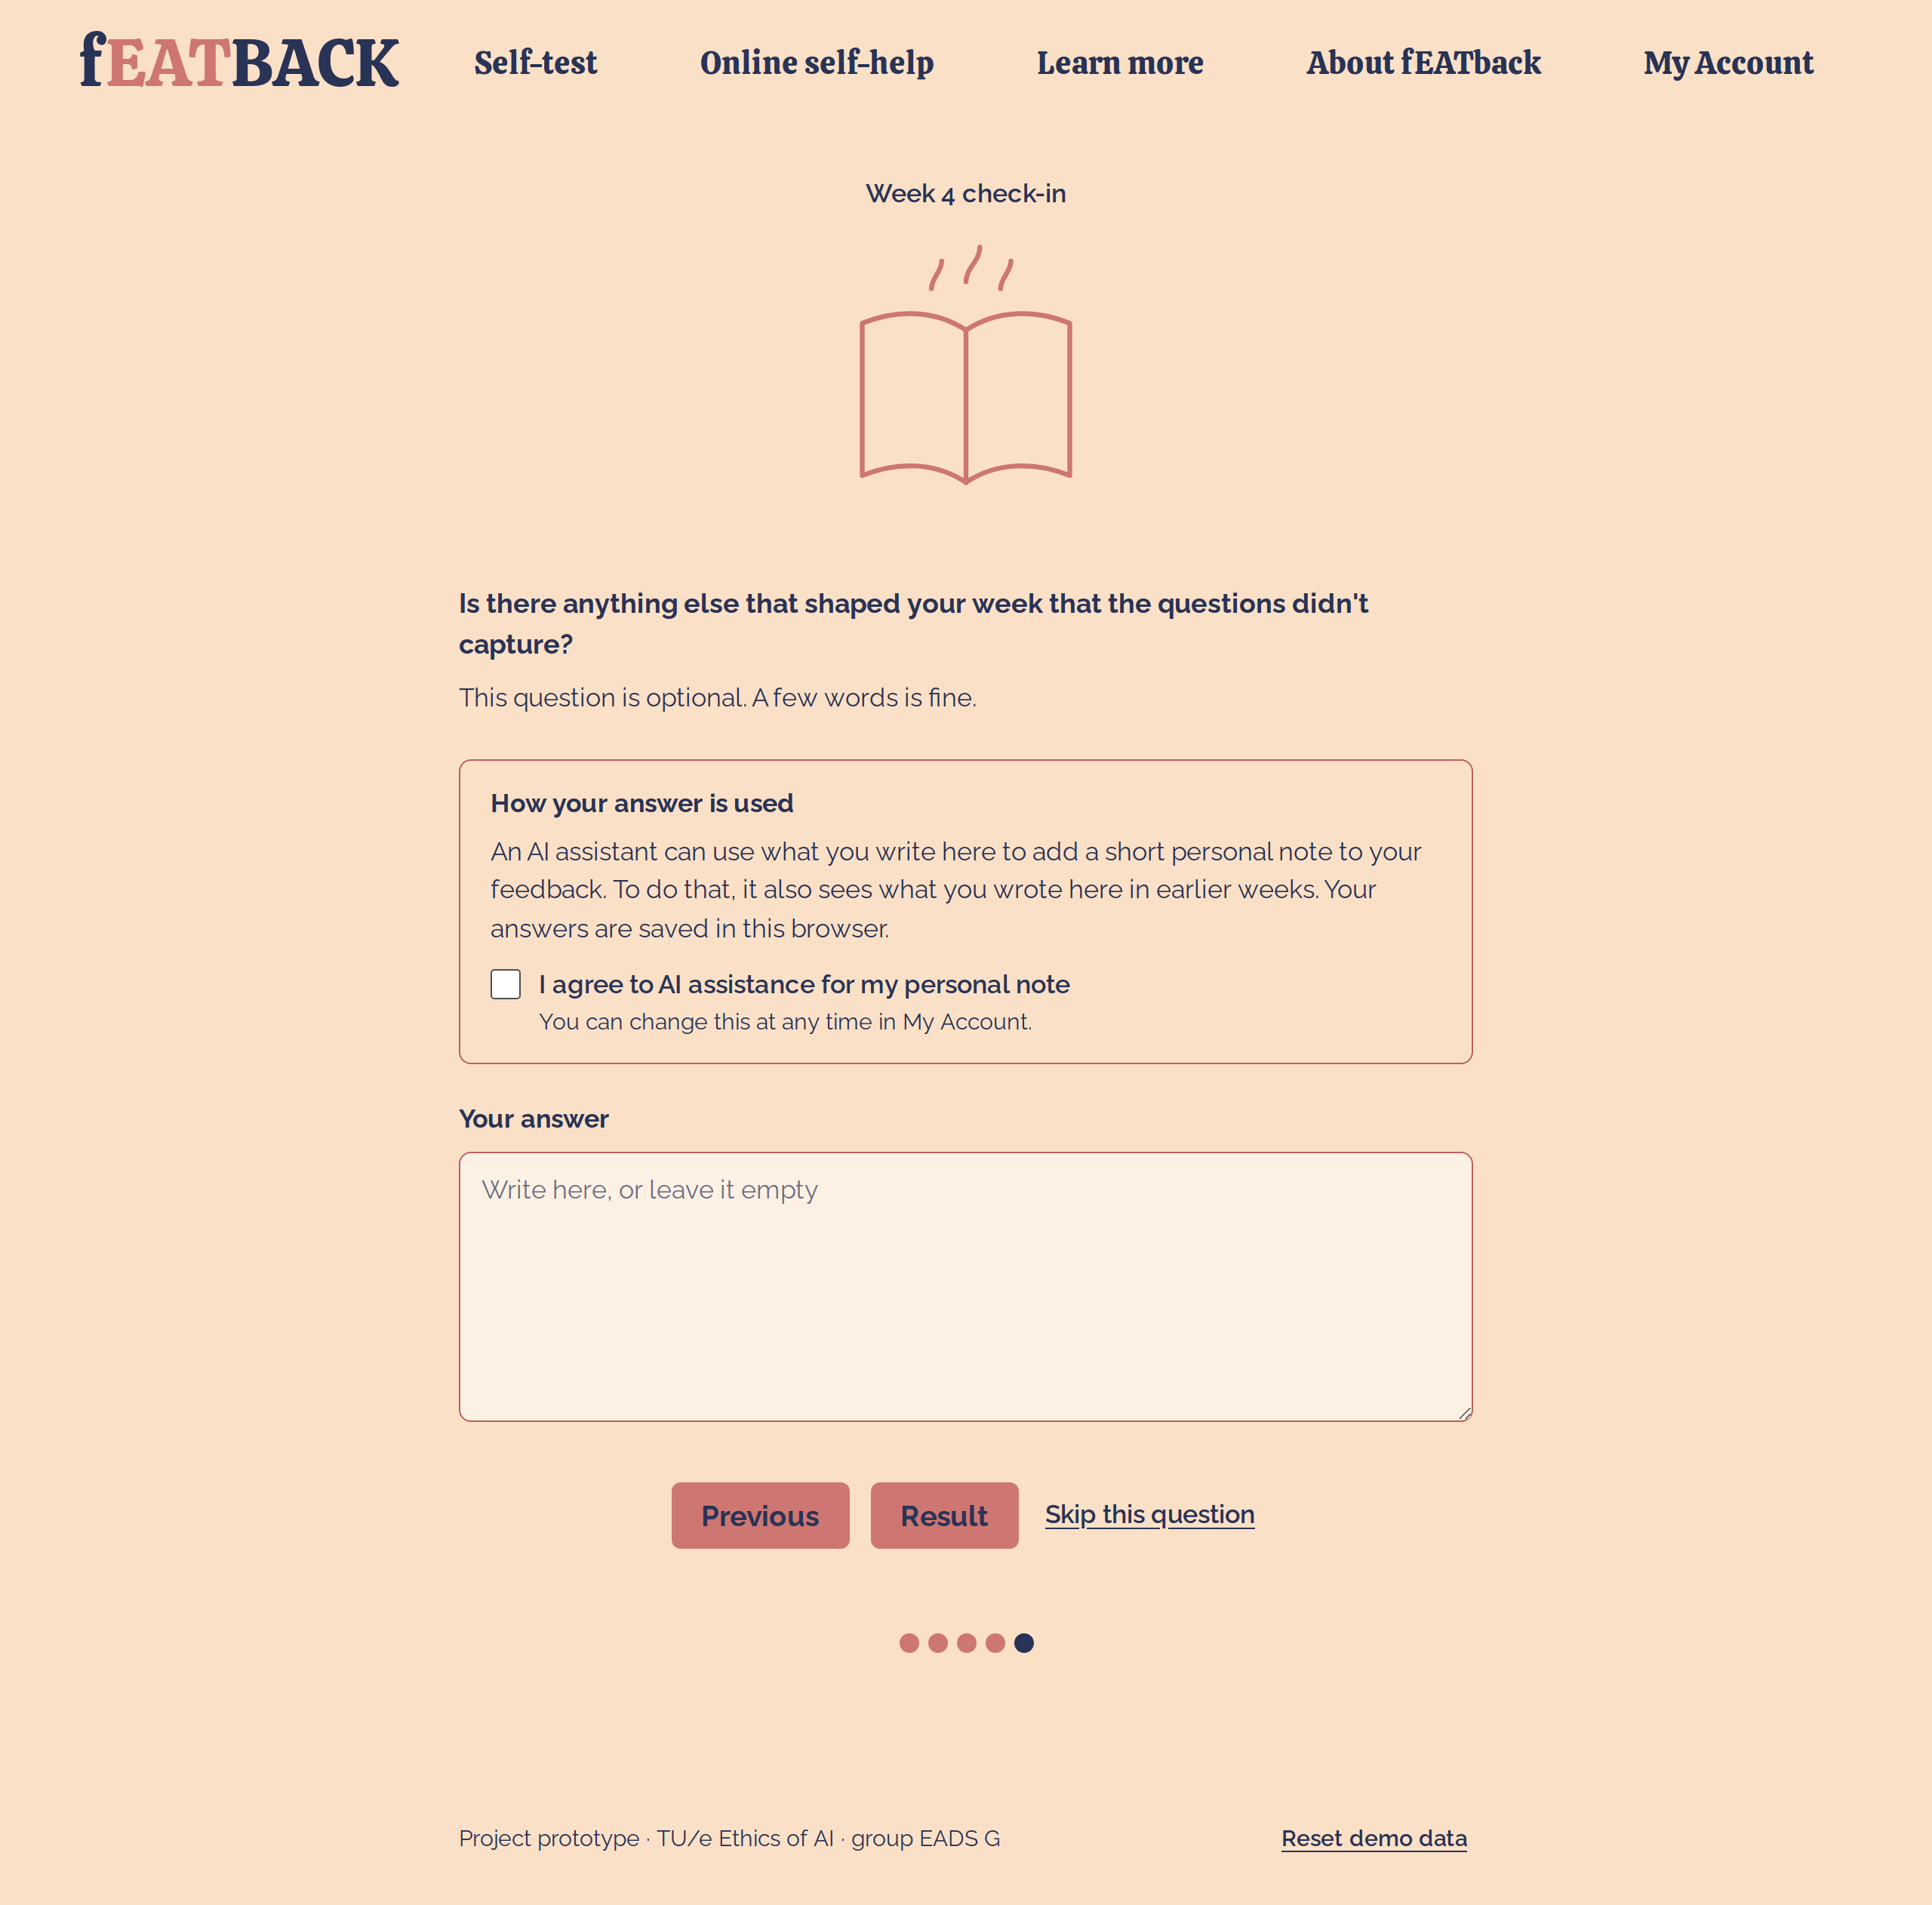
\includegraphics[width=\linewidth, trim=590 1087 590 760, clip]{q5_unticked.png}};
  \begin{scope}[x={(s.south east)}, y={(s.north west)}]
    \callout{0.979}{0.637}{1}
  \end{scope}
\end{tikzpicture}
\par\vspace{4mm}
\paneltitle{b}{Her answer and the result}
\begin{tikzpicture}
  \node[shot] (s) at (0,0) {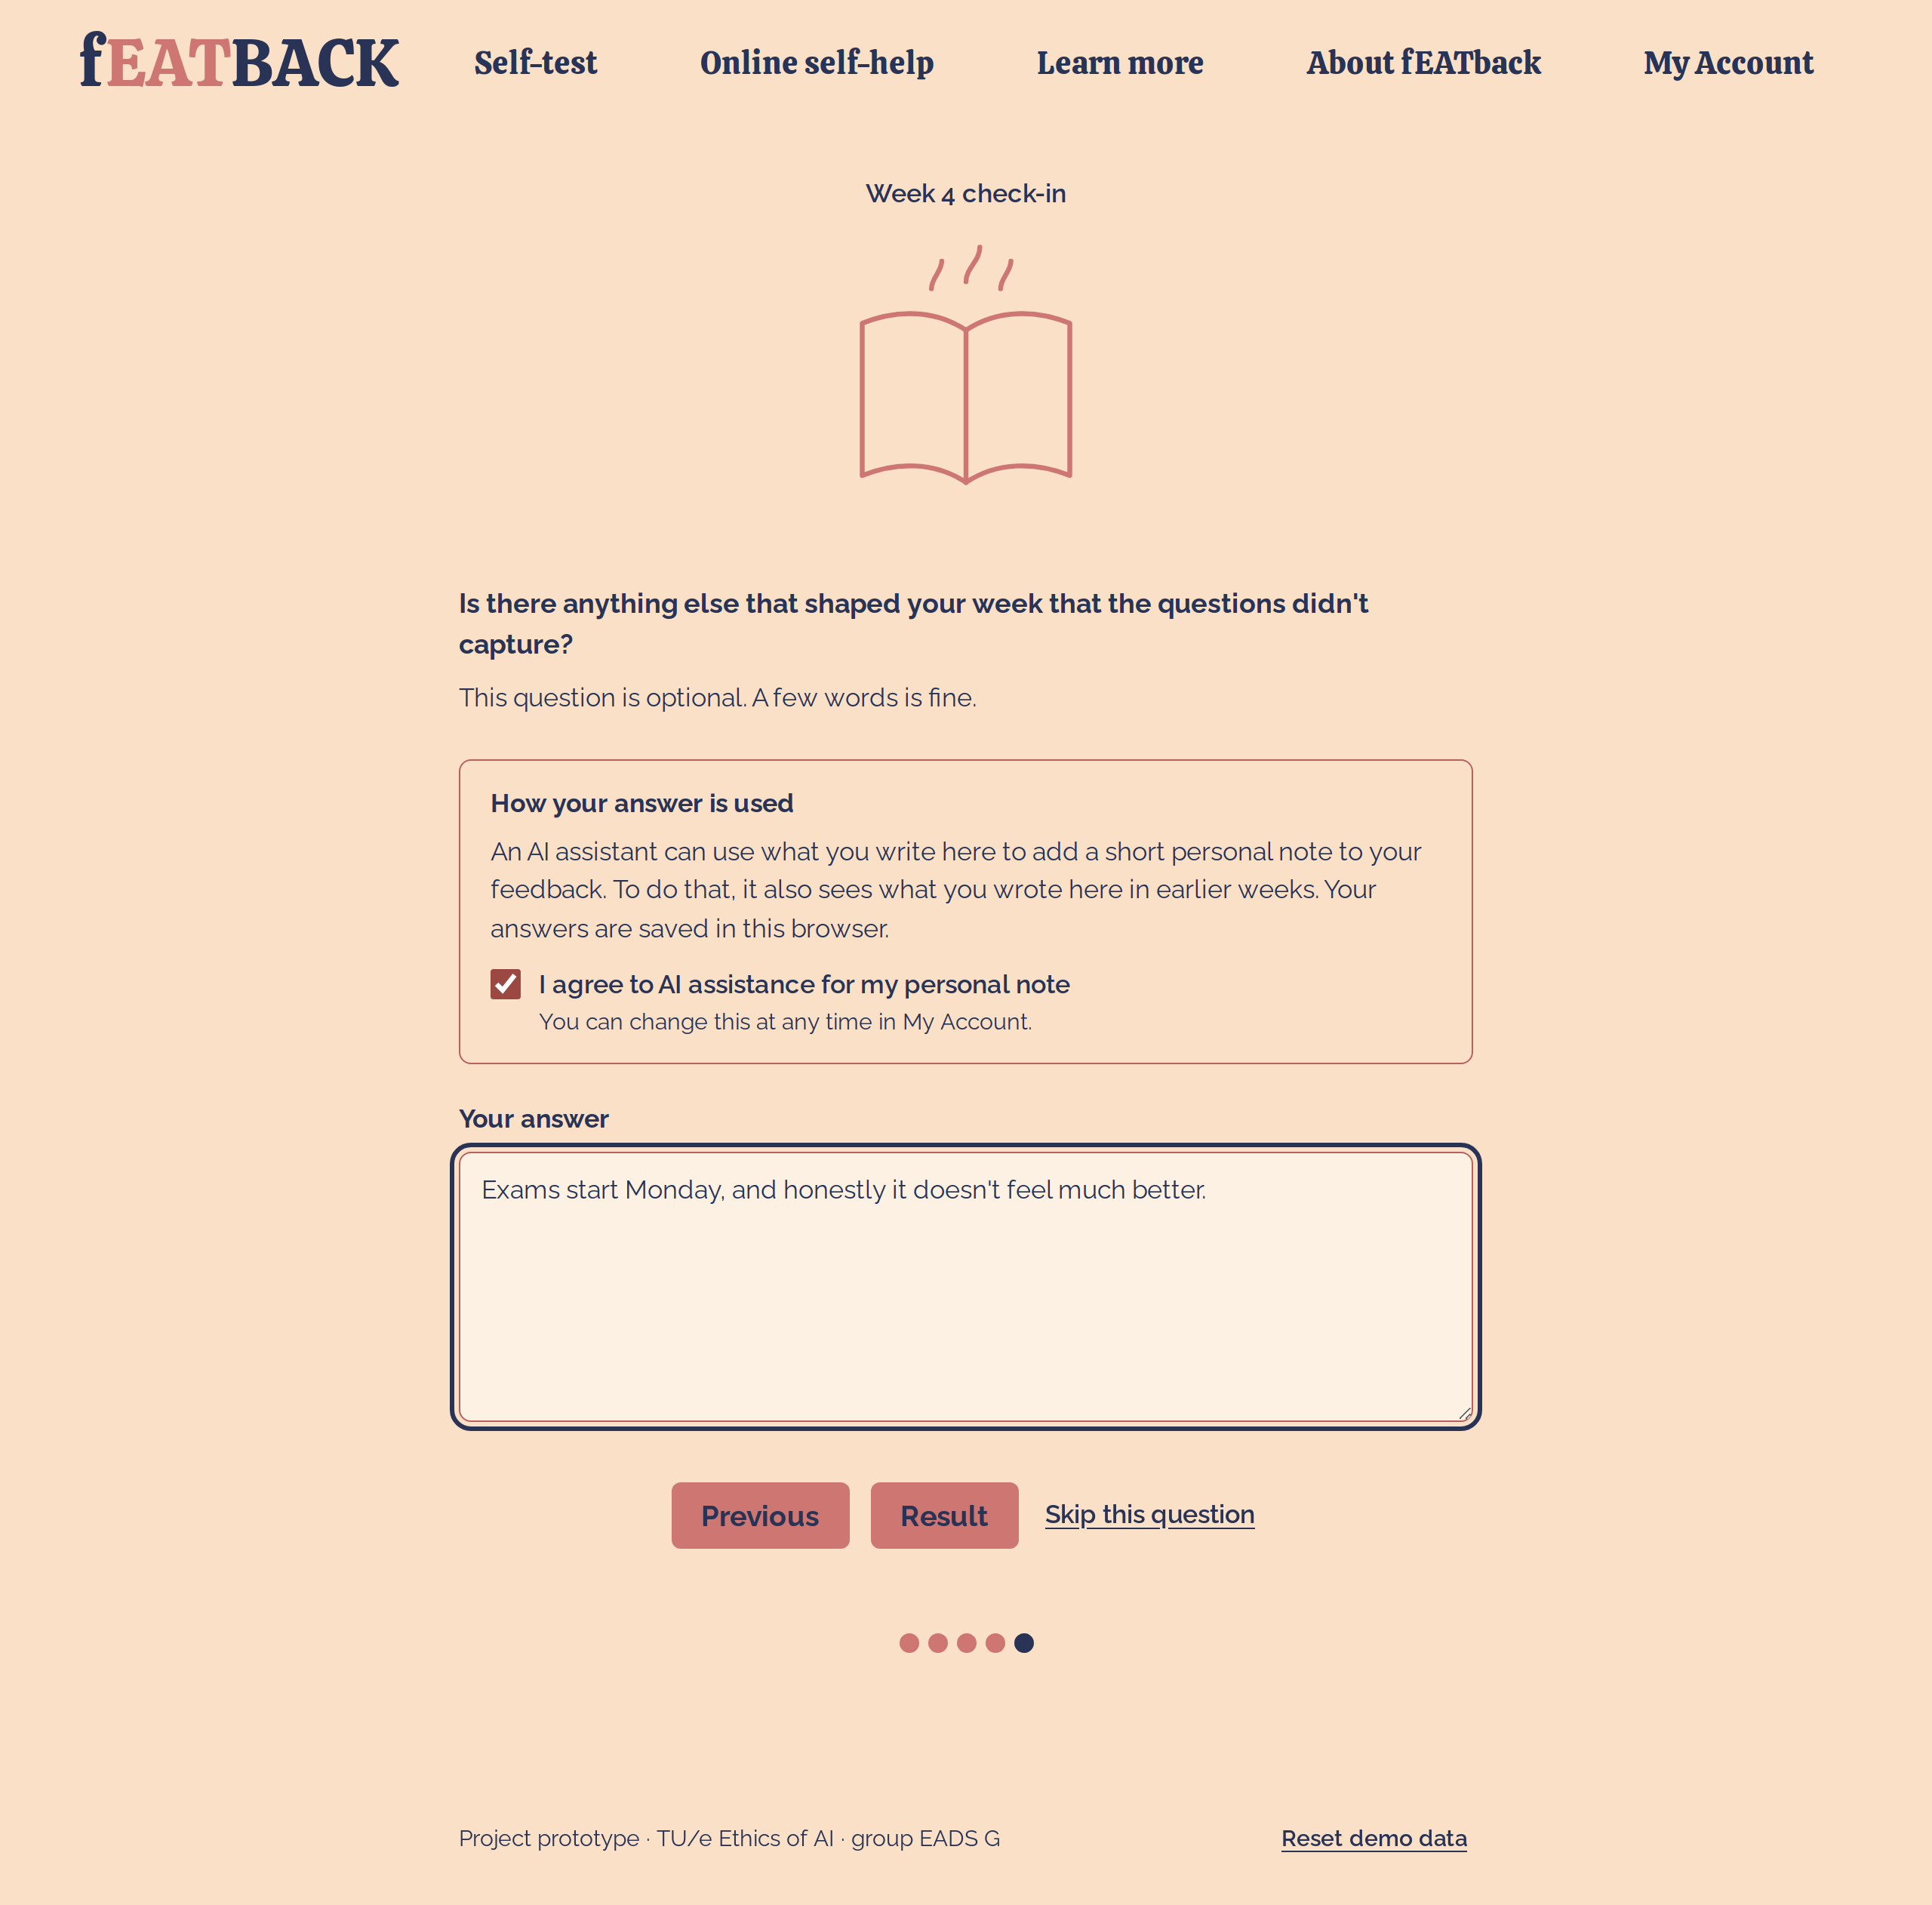
\includegraphics[width=\linewidth, trim=590 613 590 1440, clip]{q5_screen.png}};
  \begin{scope}[x={(s.south east)}, y={(s.north west)}]
    \callout{0.979}{0.817}{2}
  \end{scope}
\end{tikzpicture}
\par\vspace{1.5mm}
\begin{tikzpicture}
  \node[shot] (s) at (0,0) {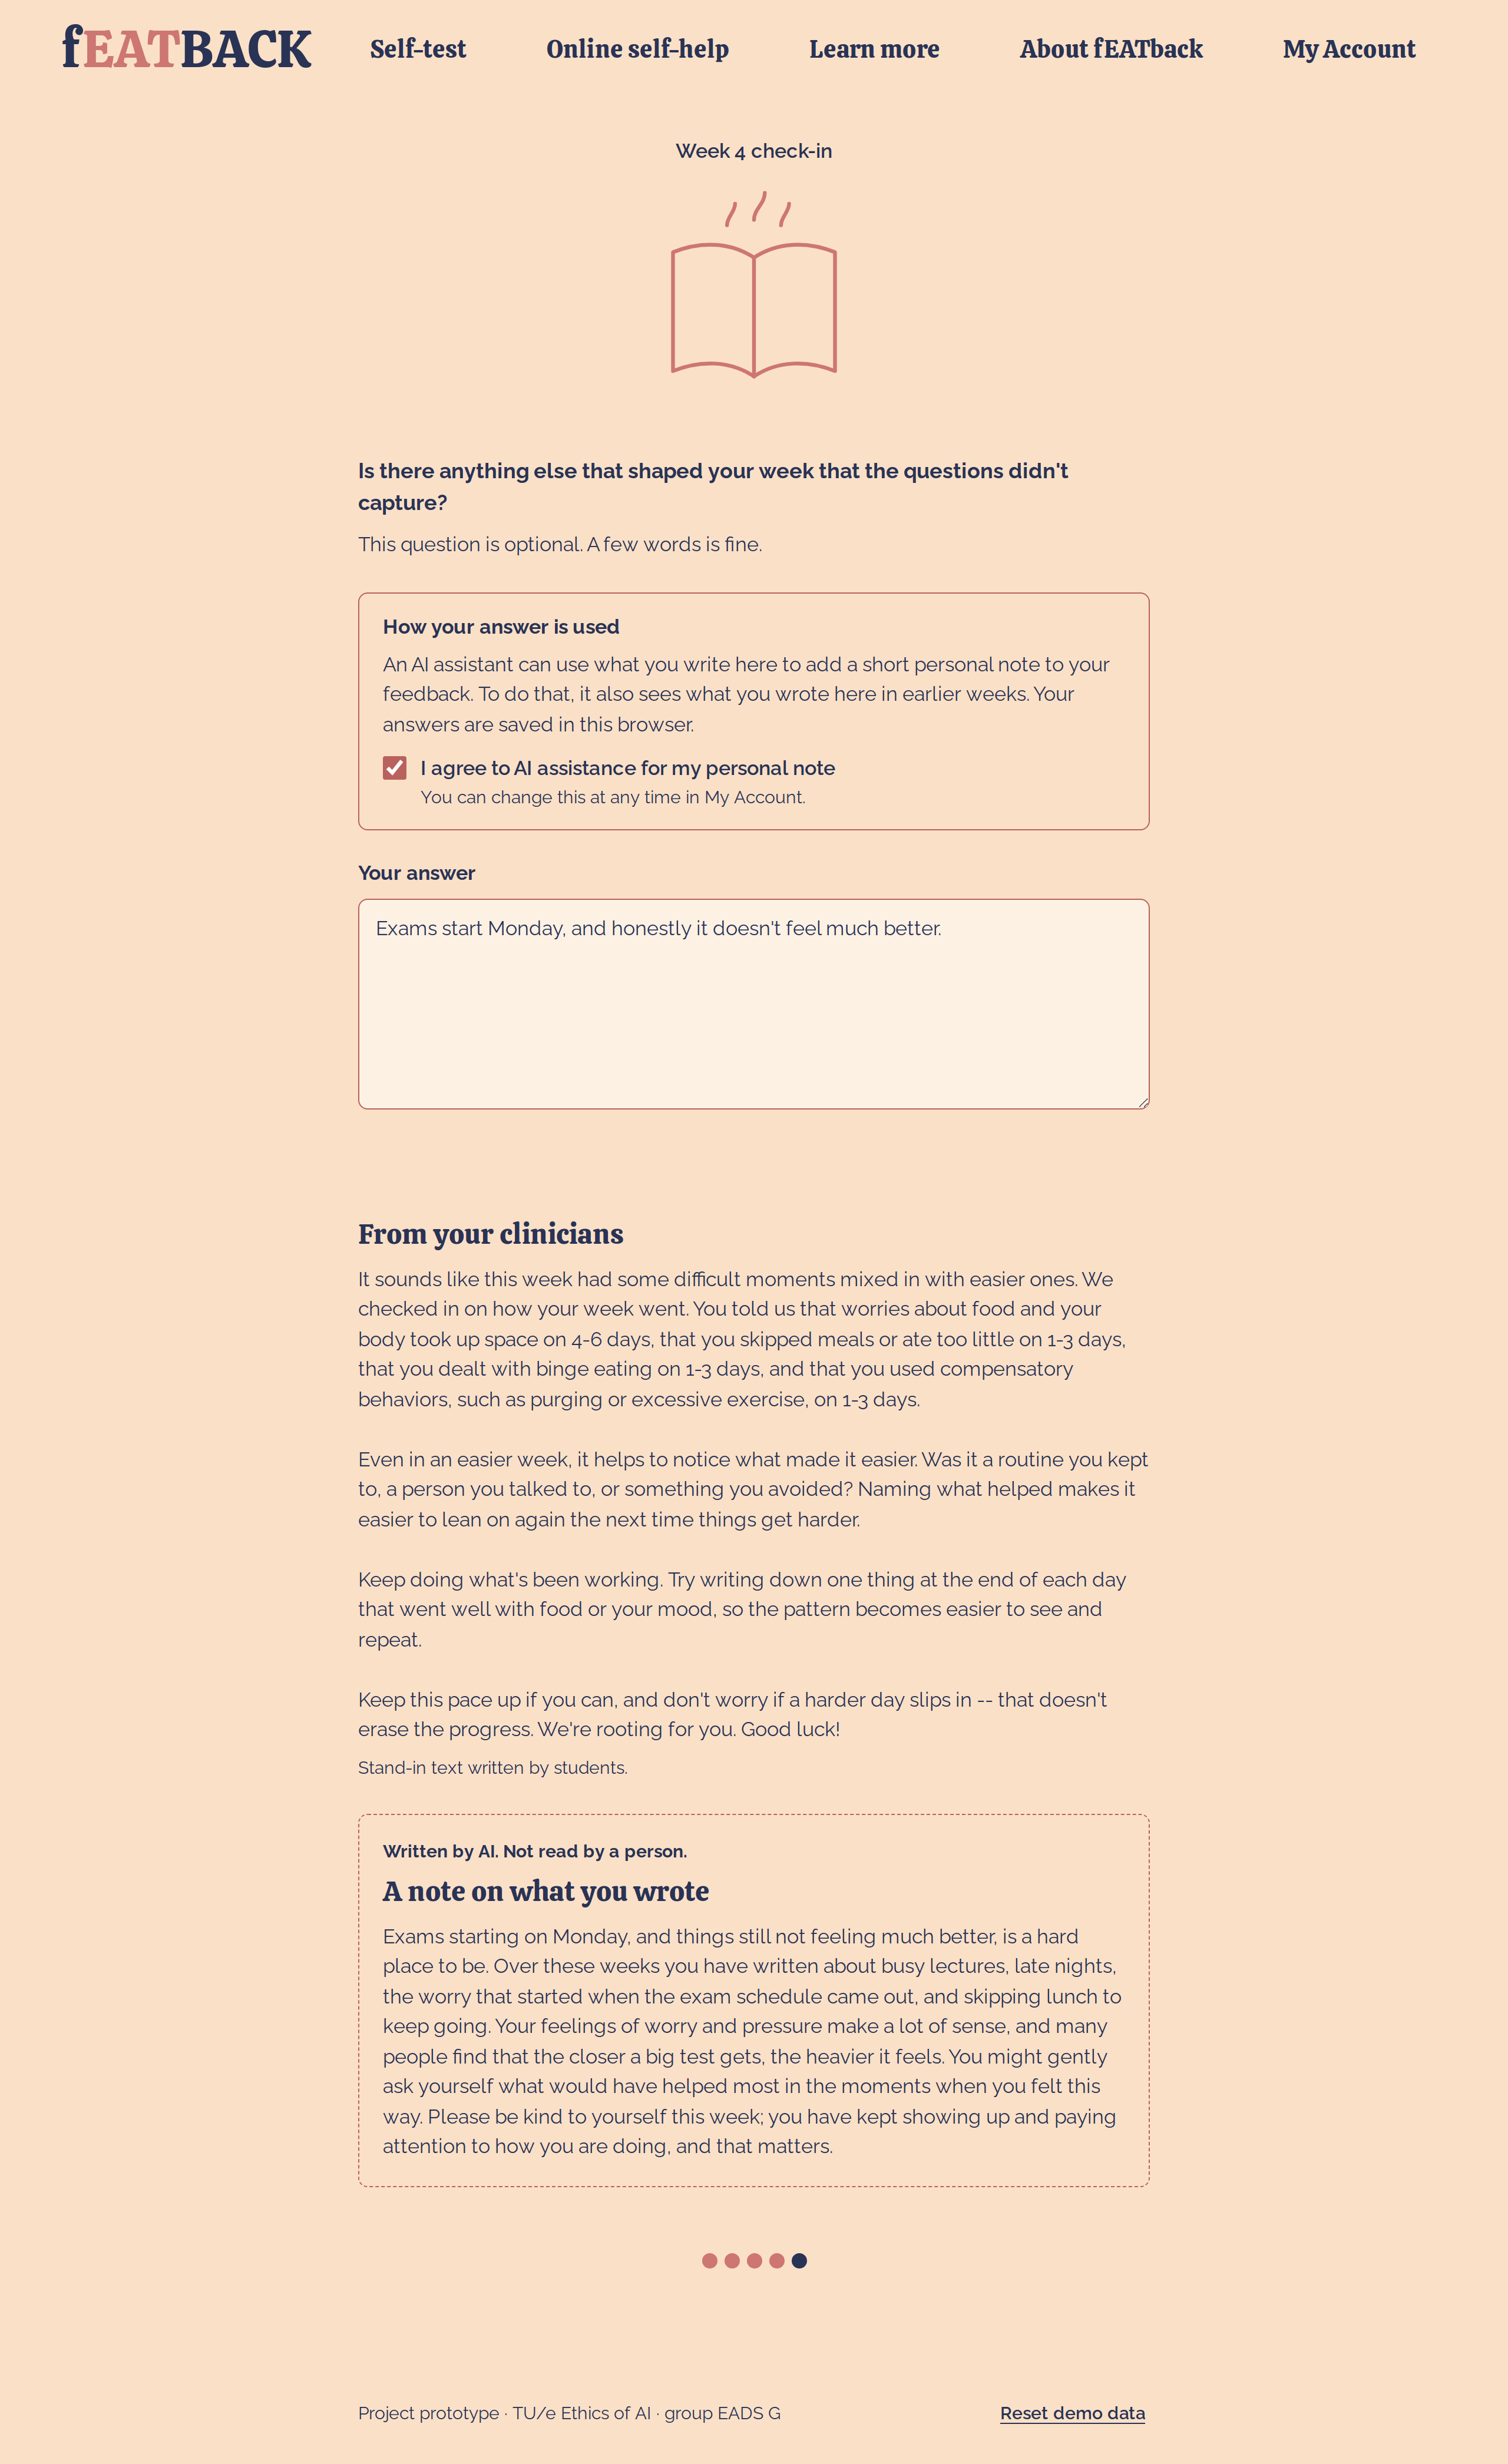
\includegraphics[width=\linewidth, trim=590 443 590 2046, clip]{result_screen.png}};
  \begin{scope}[x={(s.south east)}, y={(s.north west)}]
    \callout{0.979}{0.983}{3}
    \callout{0.979}{0.390}{4}
  \end{scope}
\end{tikzpicture}
\end{minipage}%
\hfill
% ============ Right column: other weeks and edge cases ============
\begin{minipage}[t]{0.47\textwidth}
\colhead{Week 5 and when something goes wrong}
\paneltitle{c}{Week 5, where the note looks back}
\begin{tikzpicture}
  \node[shot] (s) at (0,0) {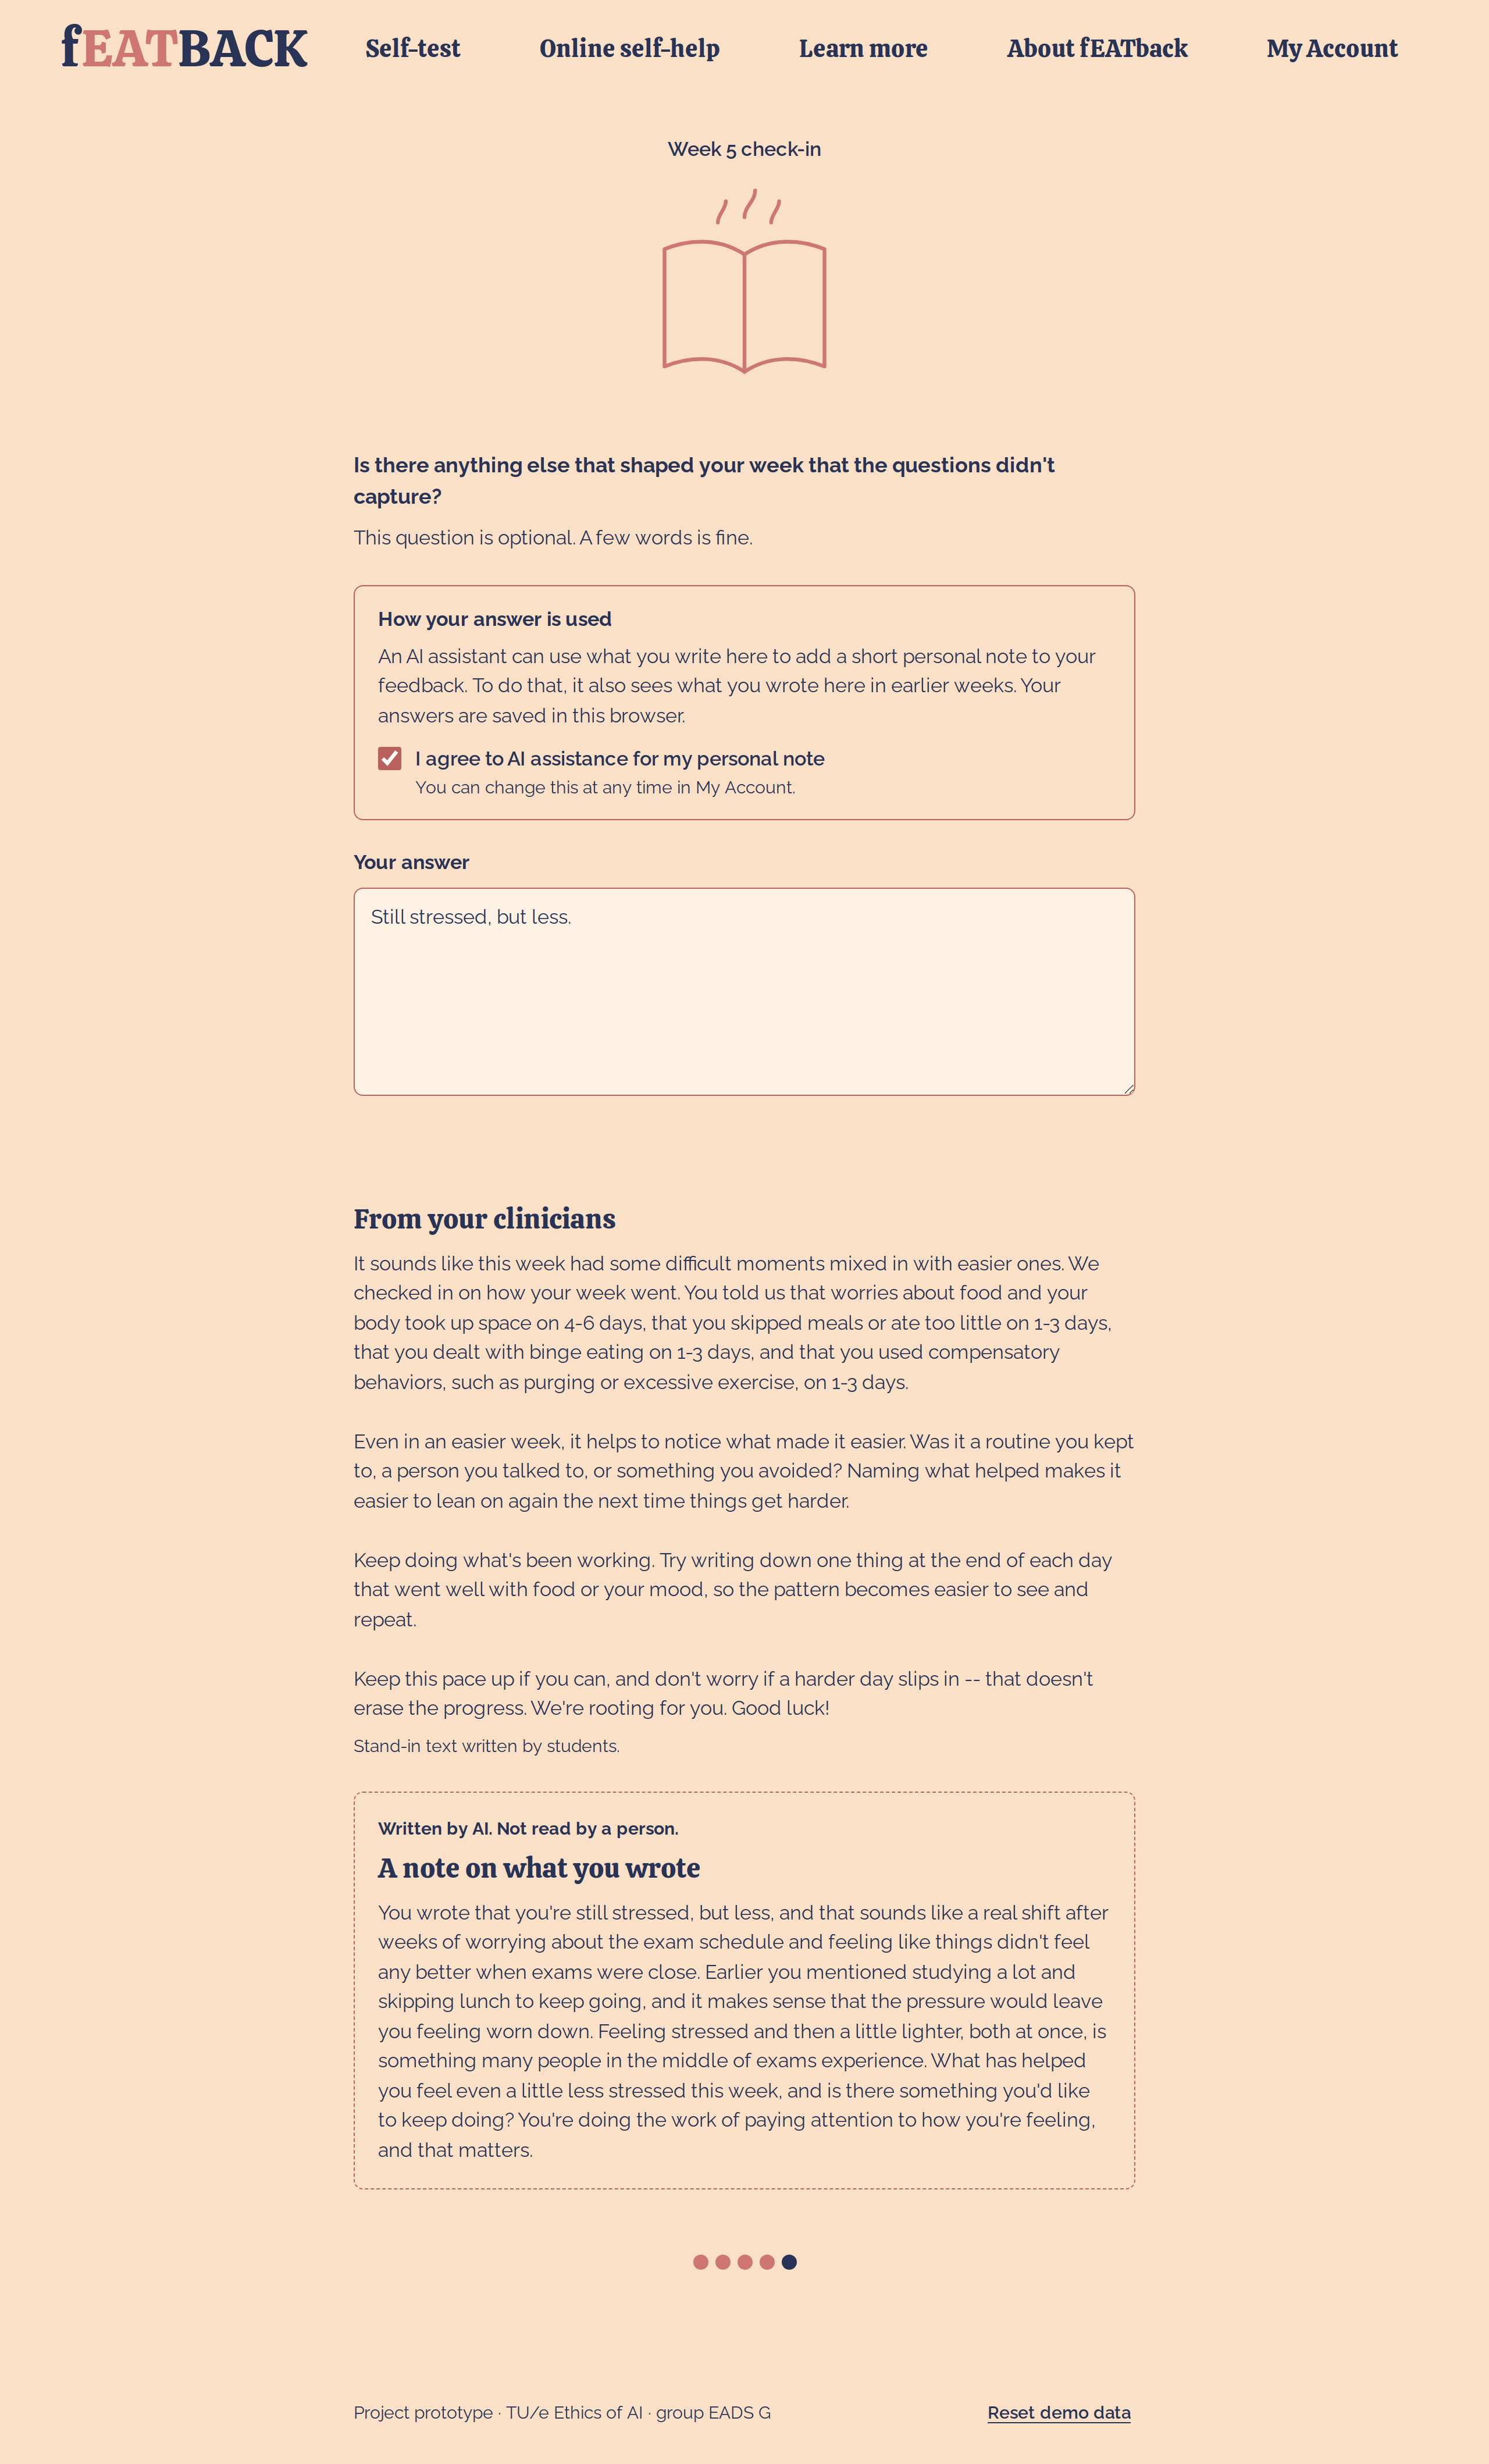
\includegraphics[width=\linewidth, trim=590 2325 590 1440, clip]{result_week5.png}};
\end{tikzpicture}
\par\vspace{1.5mm}
\begin{tikzpicture}
  \node[shot] (s) at (0,0) {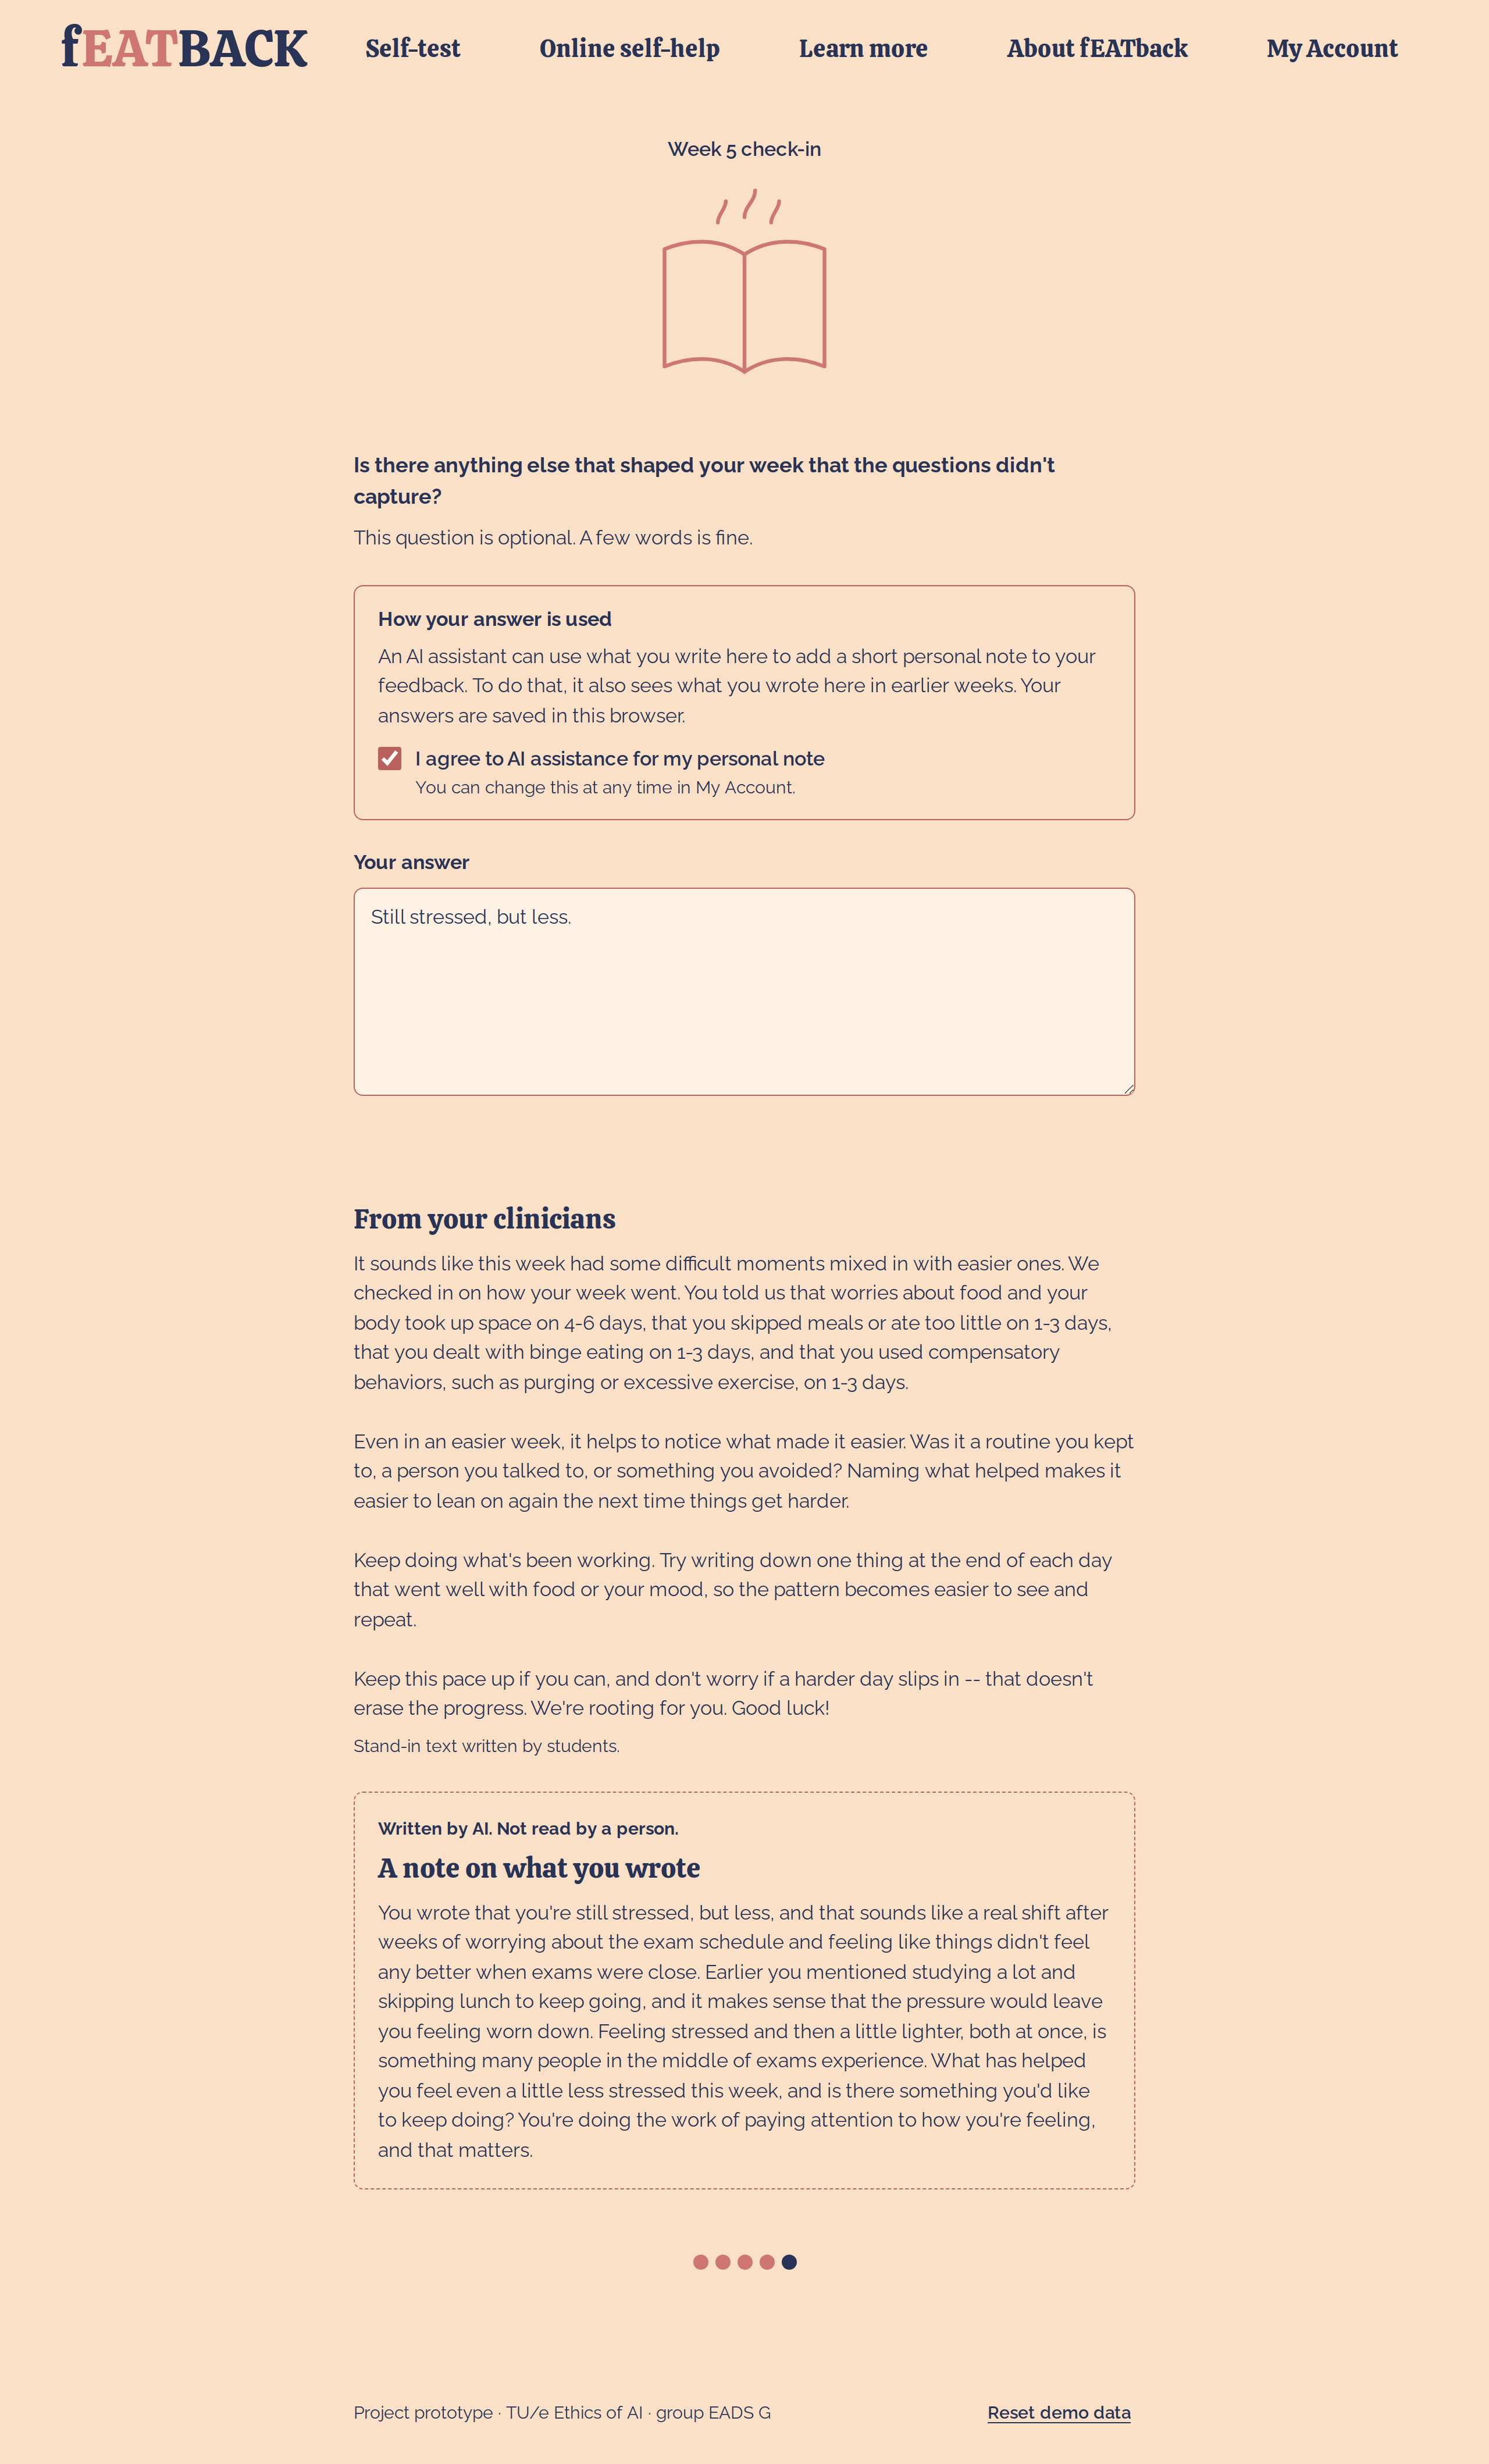
\includegraphics[width=\linewidth, trim=590 445 590 3052, clip]{result_week5.png}};
\end{tikzpicture}
\par\vspace{4mm}
\paneltitle{d}{Model off or note rejected}
\begin{tikzpicture}
  \node[shot] (s) at (0,0) {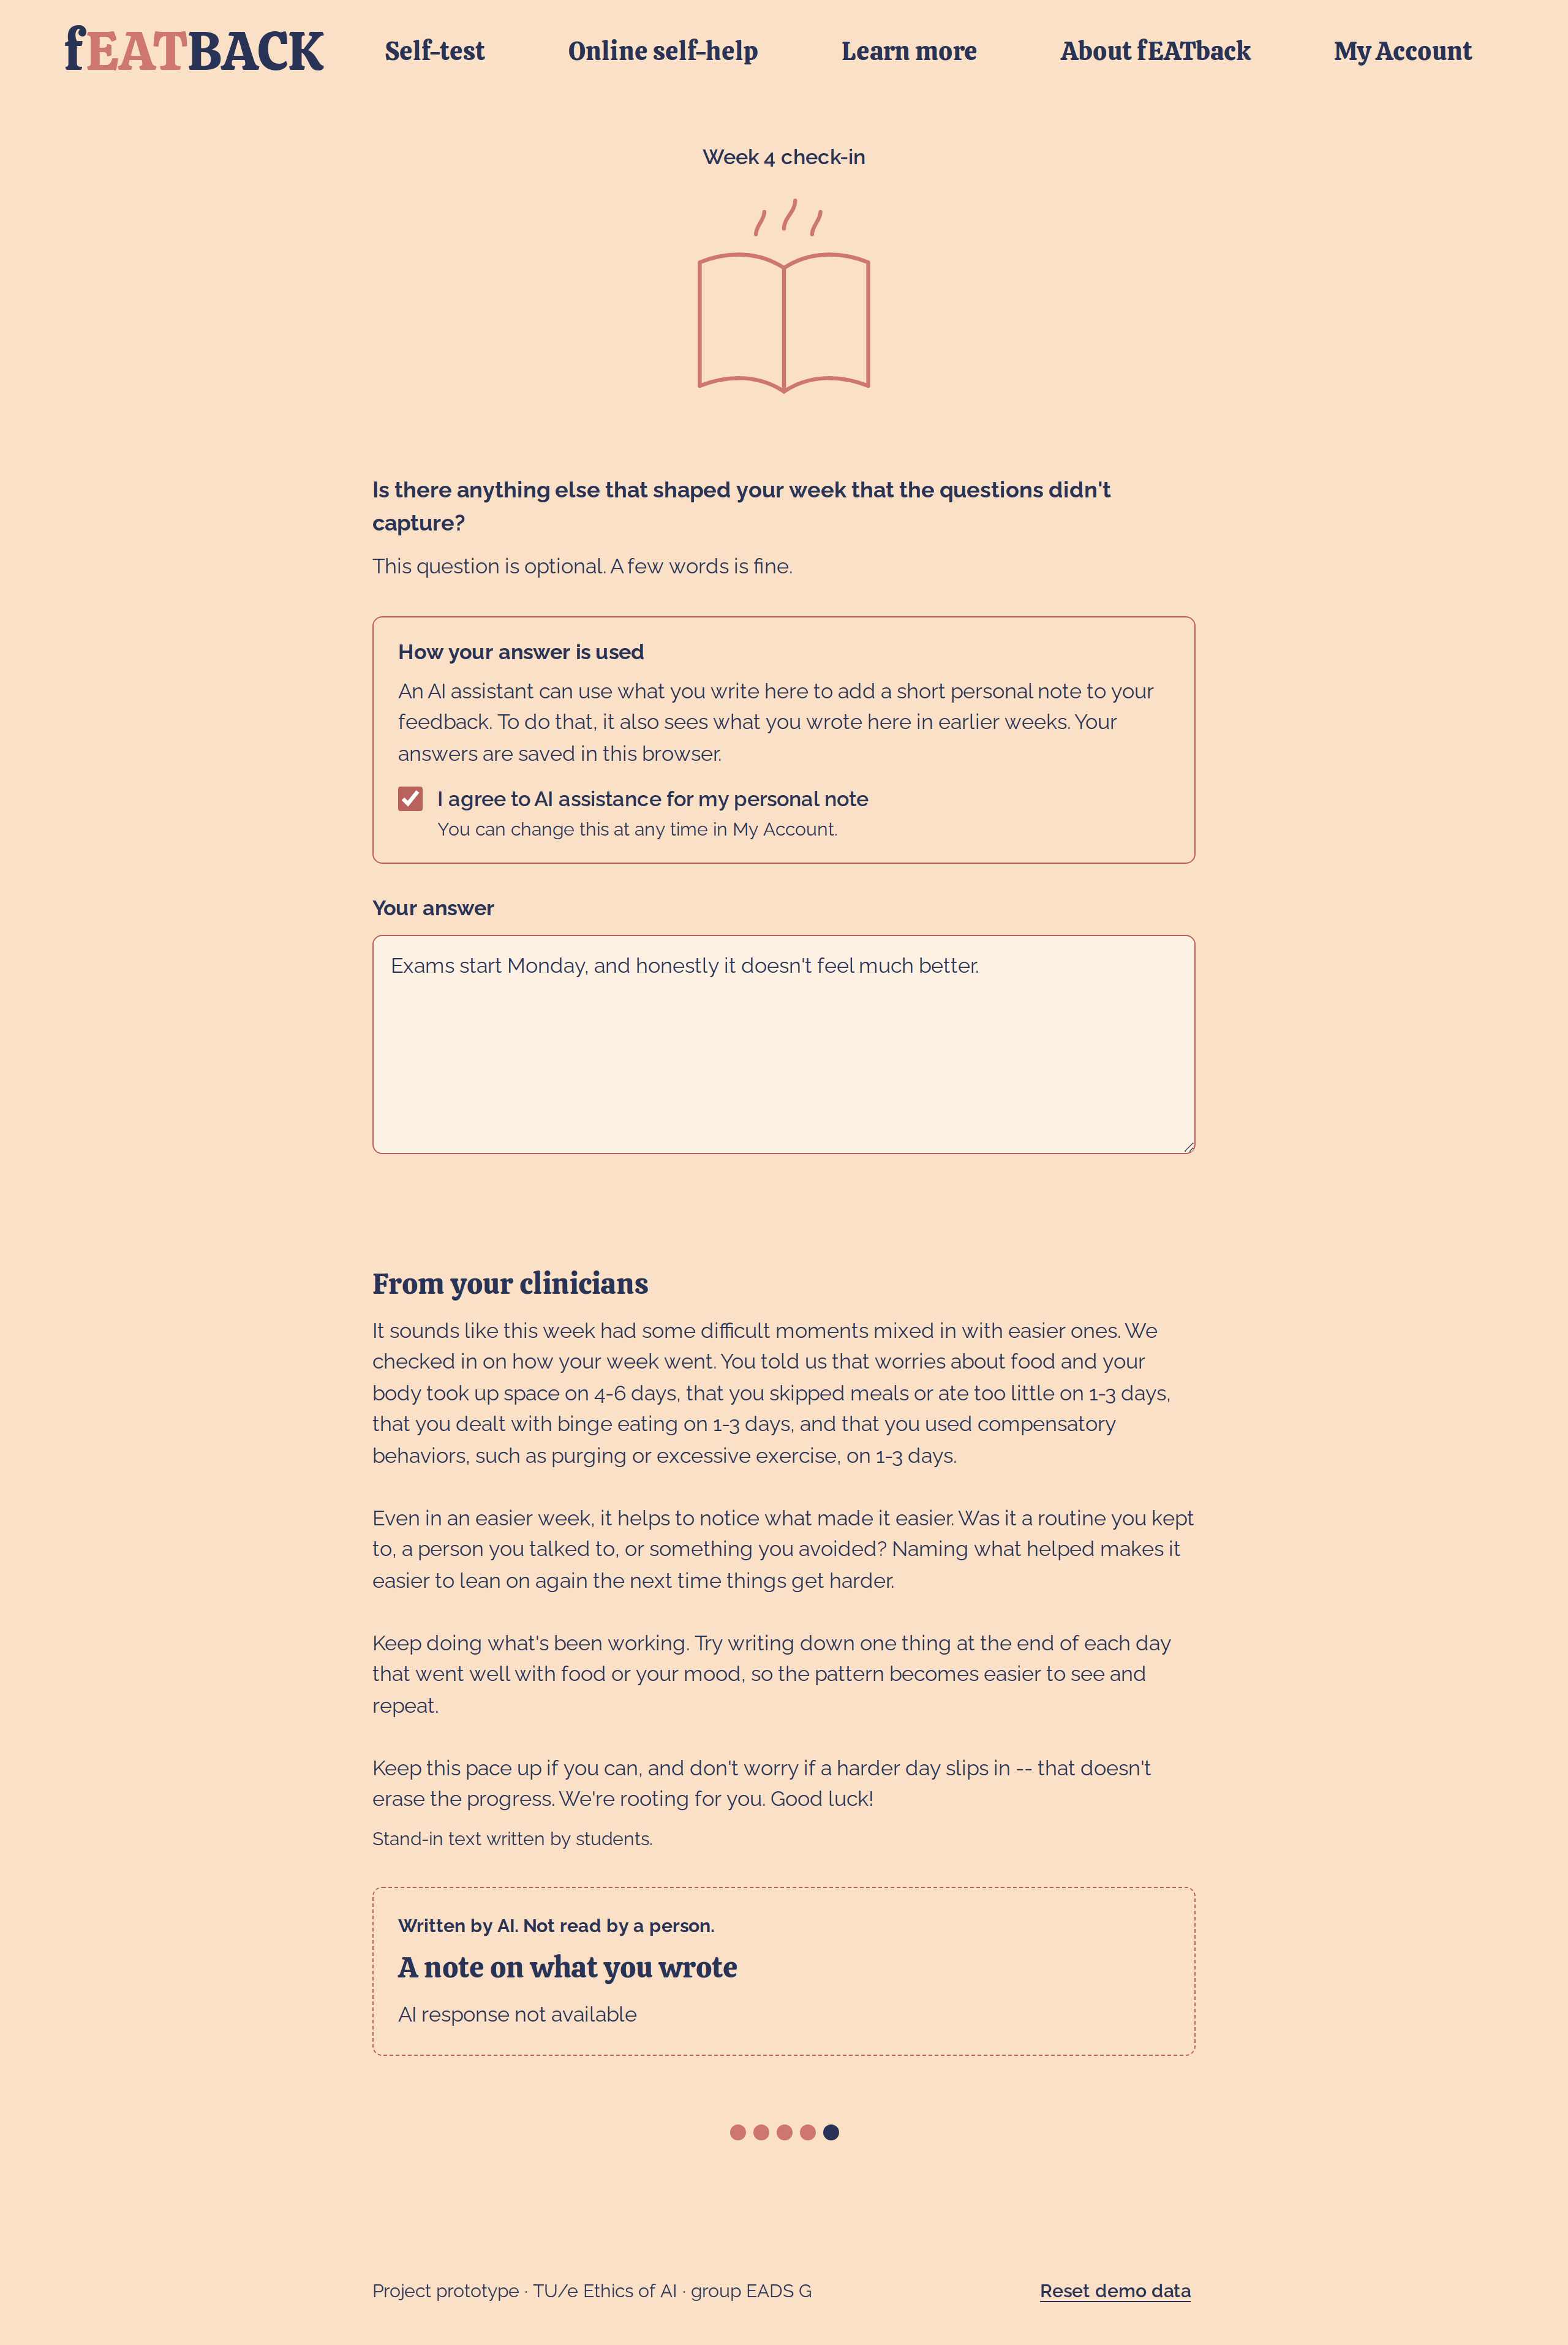
\includegraphics[width=\linewidth, trim=590 445 590 3052, clip]{fallback.png}};
  \begin{scope}[x={(s.south east)}, y={(s.north west)}]
    \callout{0.979}{0.915}{5}
  \end{scope}
\end{tikzpicture}
\par\vspace{4mm}
\paneltitle{e}{An answer with signs of acute risk}
\begin{tikzpicture}
  \node[shot] (s) at (0,0) {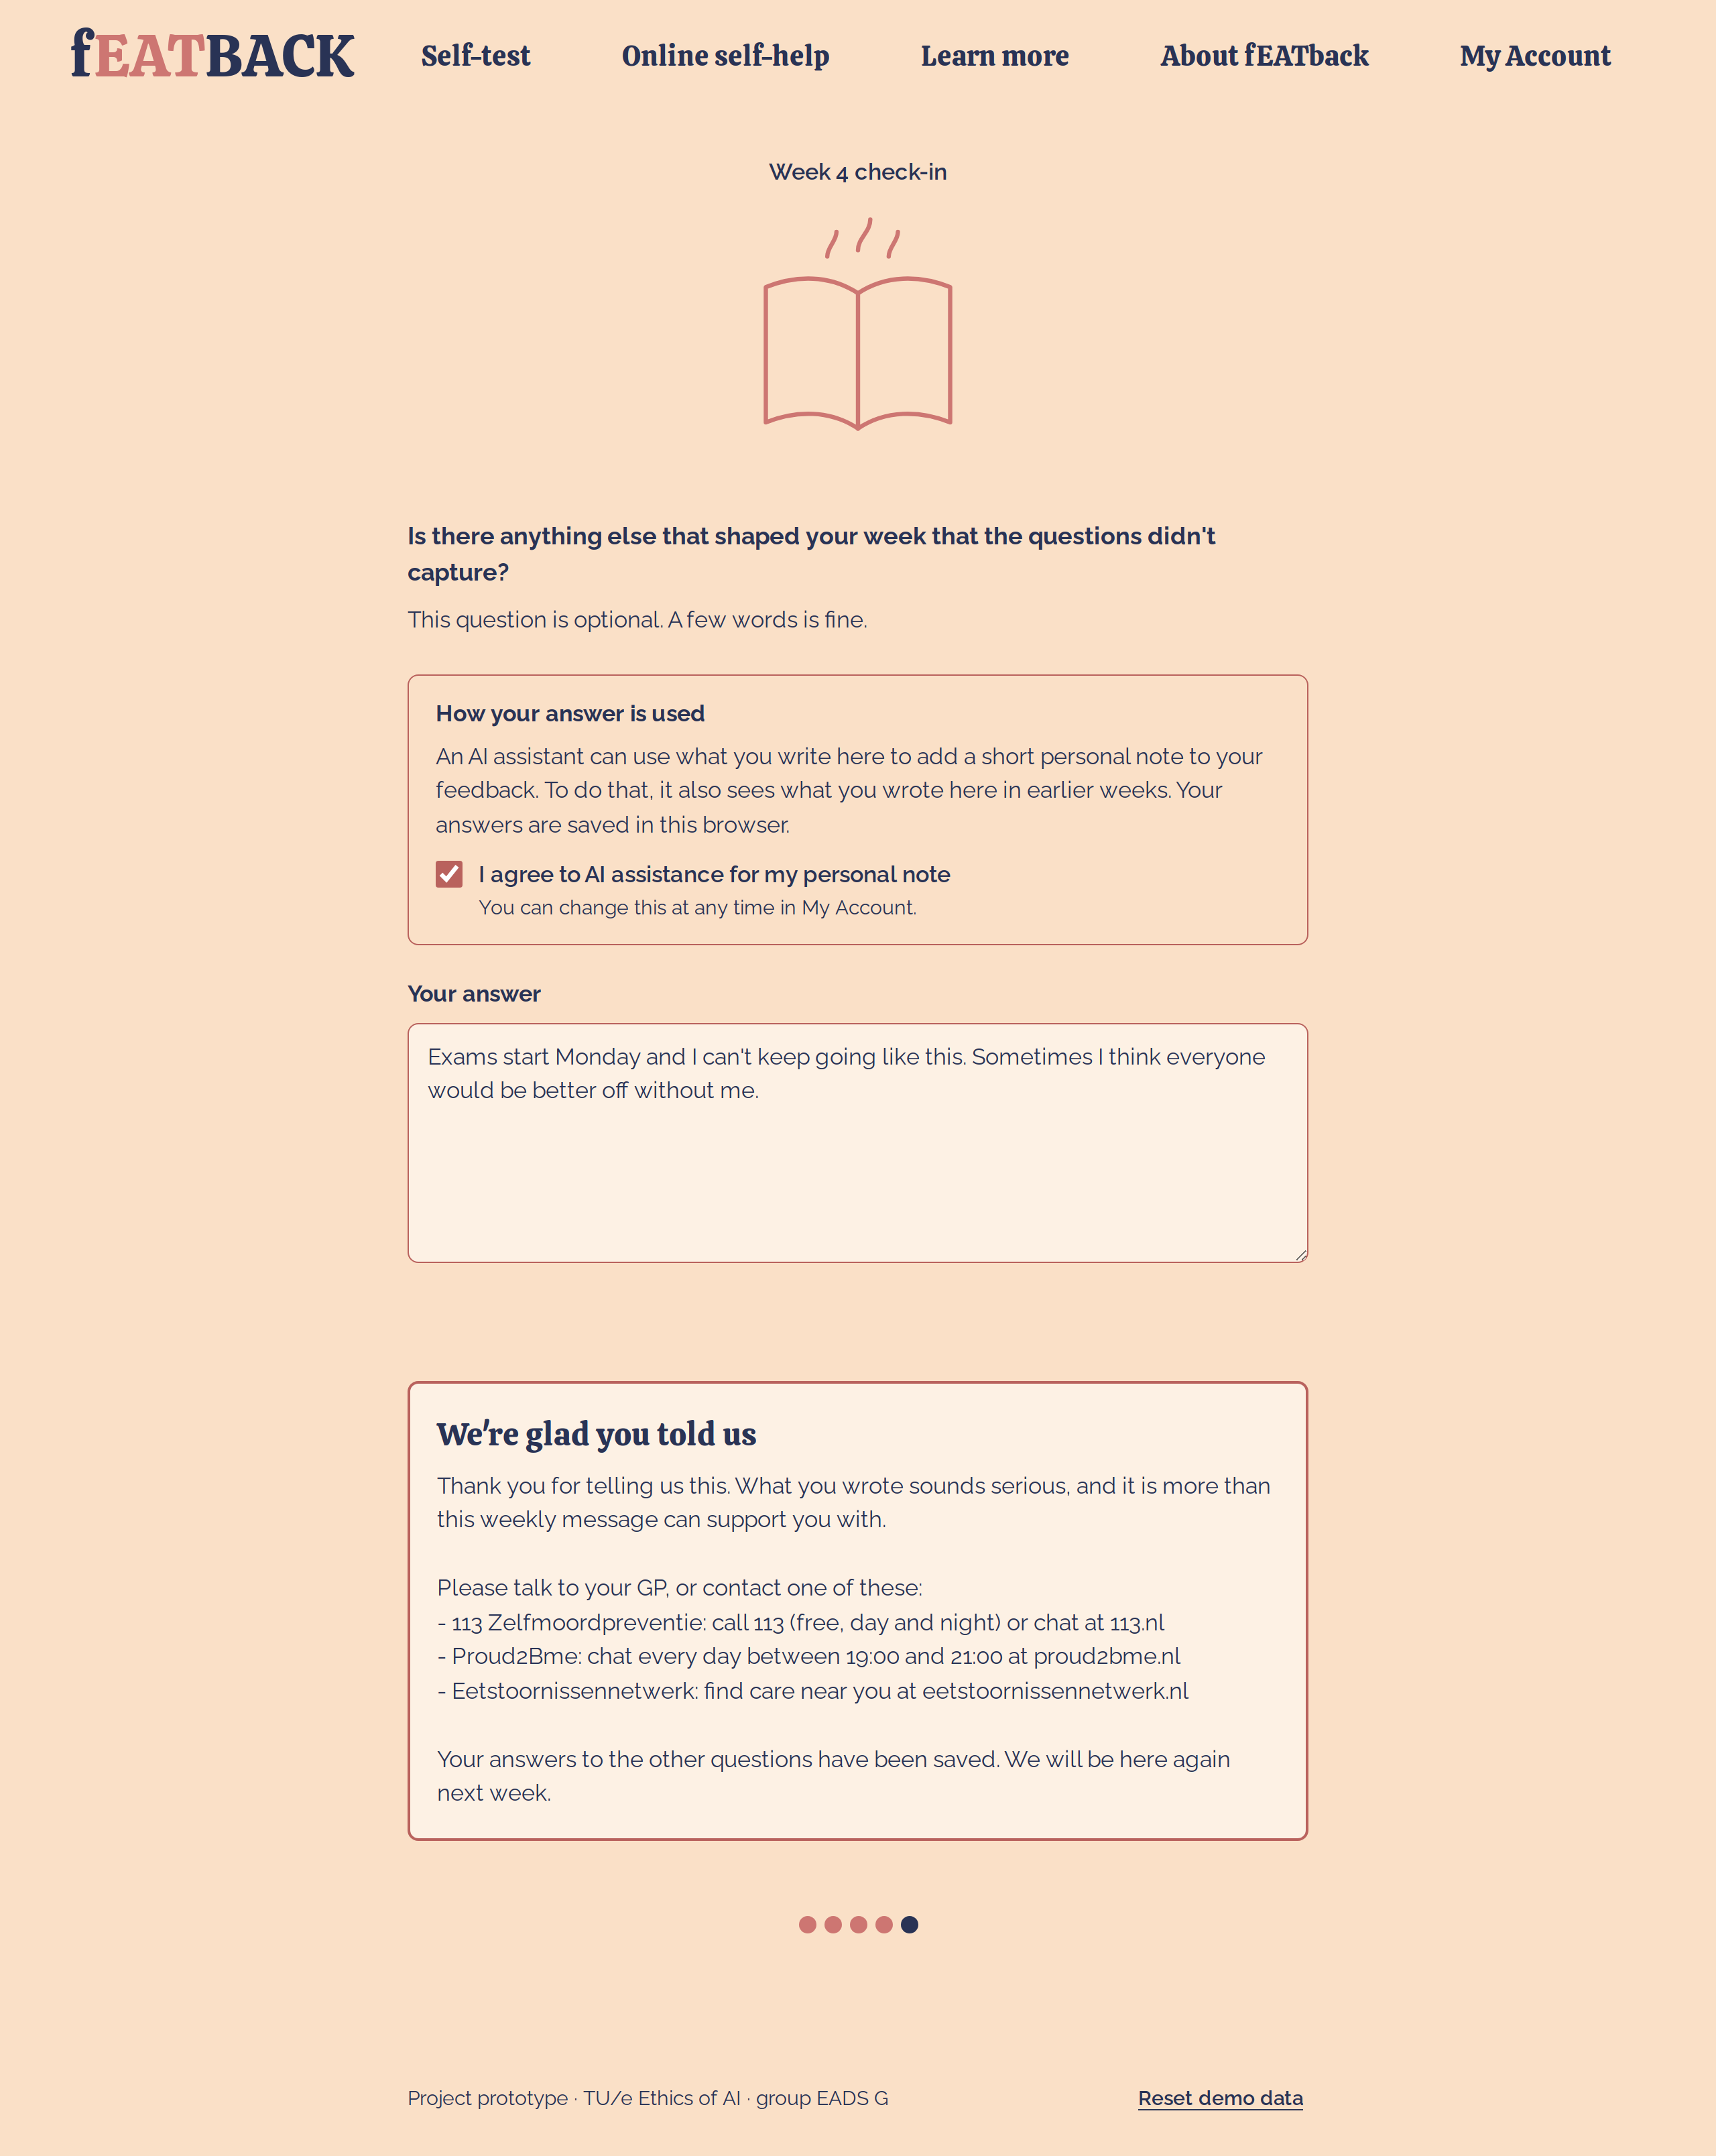
\includegraphics[width=\linewidth, trim=590 1305 590 1440, clip]{acute.png}};
\end{tikzpicture}
\par\vspace{1.5mm}
\begin{tikzpicture}
  \node[shot] (s) at (0,0) {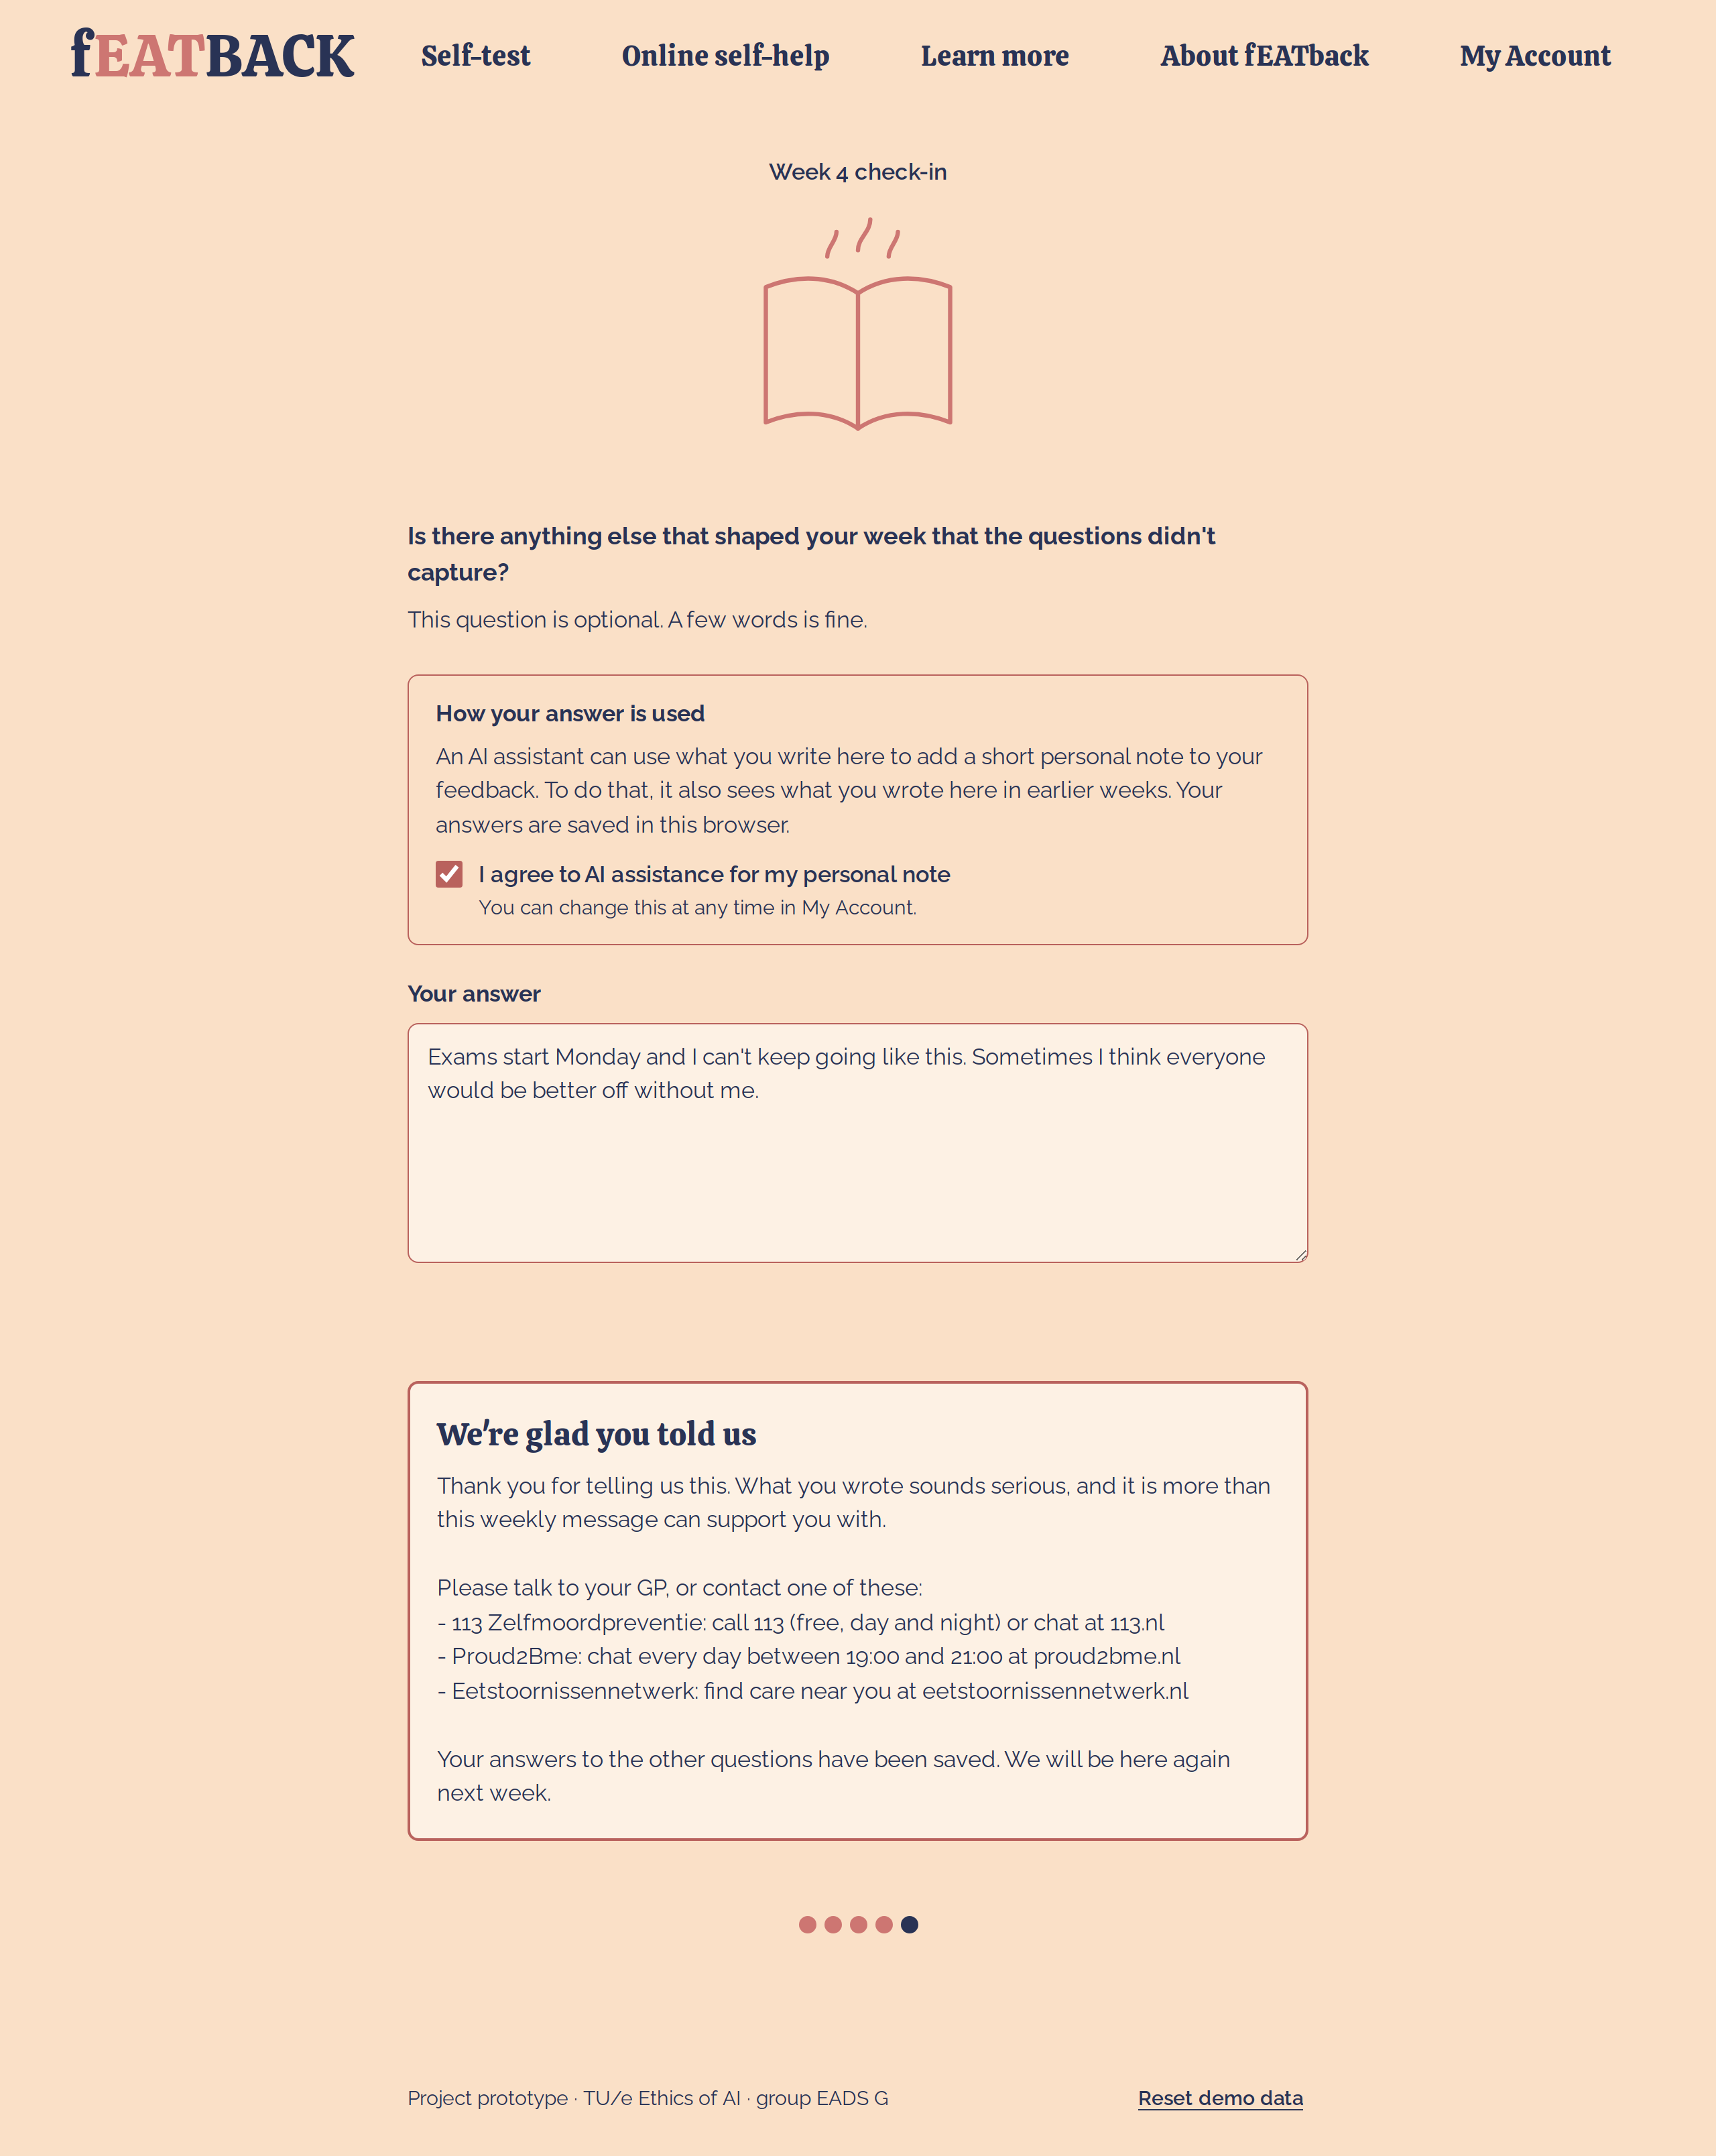
\includegraphics[width=\linewidth, trim=590 443 590 2032, clip]{acute.png}};
  \begin{scope}[x={(s.south east)}, y={(s.north west)}]
    \callout{0.979}{0.962}{6}
  \end{scope}
\end{tikzpicture}
\end{minipage}

\vspace{5mm}
% ---- Key: one entry per callout, aligned with the two columns ----
\newcommand{\keyline}[2]{\key{#1}\hspace{2mm}#2\par\vspace{1.2mm}}
{\footnotesize\sffamily
\begin{minipage}[t]{0.47\textwidth}
\keyline{1}{Consent box starts unticked (part 3)}
\keyline{2}{Answer stored for the trend (part 3)}
\keyline{3}{Stand-in bank message (part 1)}
\end{minipage}\hfill
\begin{minipage}[t]{0.47\textwidth}
\keyline{4}{Label on every AI note (part 2)}
\keyline{5}{Fixed fallback text we wrote (part 1)}
\keyline{6}{Gate takes the more severe label (part 1)}
\end{minipage}}

\vspace{2mm}
\caption{Maren's check-ins from Section~\ref{sec:narrative} as they appear on screen. Part numbers in the key
point to the Responsible Innovation statement. The AI notes in (b) and (c) are real
output from our fine-tuned writer model, run on 12 October 2026. The bank message, Maren
and her earlier answers are made up for the demo.}
\label{fig:mockup}
\end{figure}
.
% Needs tikz (loaded by todonotes in main.tex), graphicx and float.

% ---- Figure style ----------------------------------------------------------
\definecolor{fbnavy}{HTML}{283357}
\tikzset{
  shot/.style={anchor=south west, inner sep=0, draw=black!18, line width=0.4pt},
  callout/.style={circle, fill=fbnavy, draw=white, line width=0.9pt, text=white,
    font=\sffamily\bfseries\scriptsize, inner sep=0pt, minimum size=4.4mm}}
% Callouts always sit on the top-right corner of the card they mark.
\newcommand{\callout}[3]{\node[callout, overlay] at (#1,#2) {#3};}
% Inline callout for the key
\newcommand{\key}[1]{\tikz[baseline=-0.6ex]\node[callout]{#1};}
% Panel title
\newcommand{\paneltitle}[2]{{\sffamily\footnotesize\color{fbnavy}\textbf{(#1)}~#2}\par\vspace{1mm}}
\newcommand{\colhead}[1]{{\sffamily\small\bfseries\color{fbnavy}#1}\par\vspace{0.5mm}{\color{black!25}\hrule height 0.4pt}\vspace{2mm}}

\begin{figure}[H]
\centering
% ============ Left column: week 4, the usual path ============
\begin{minipage}[t]{0.47\textwidth}
\colhead{Week 4}
\paneltitle{a}{Question 5, before she agrees}
\begin{tikzpicture}
  \node[shot] (s) at (0,0) {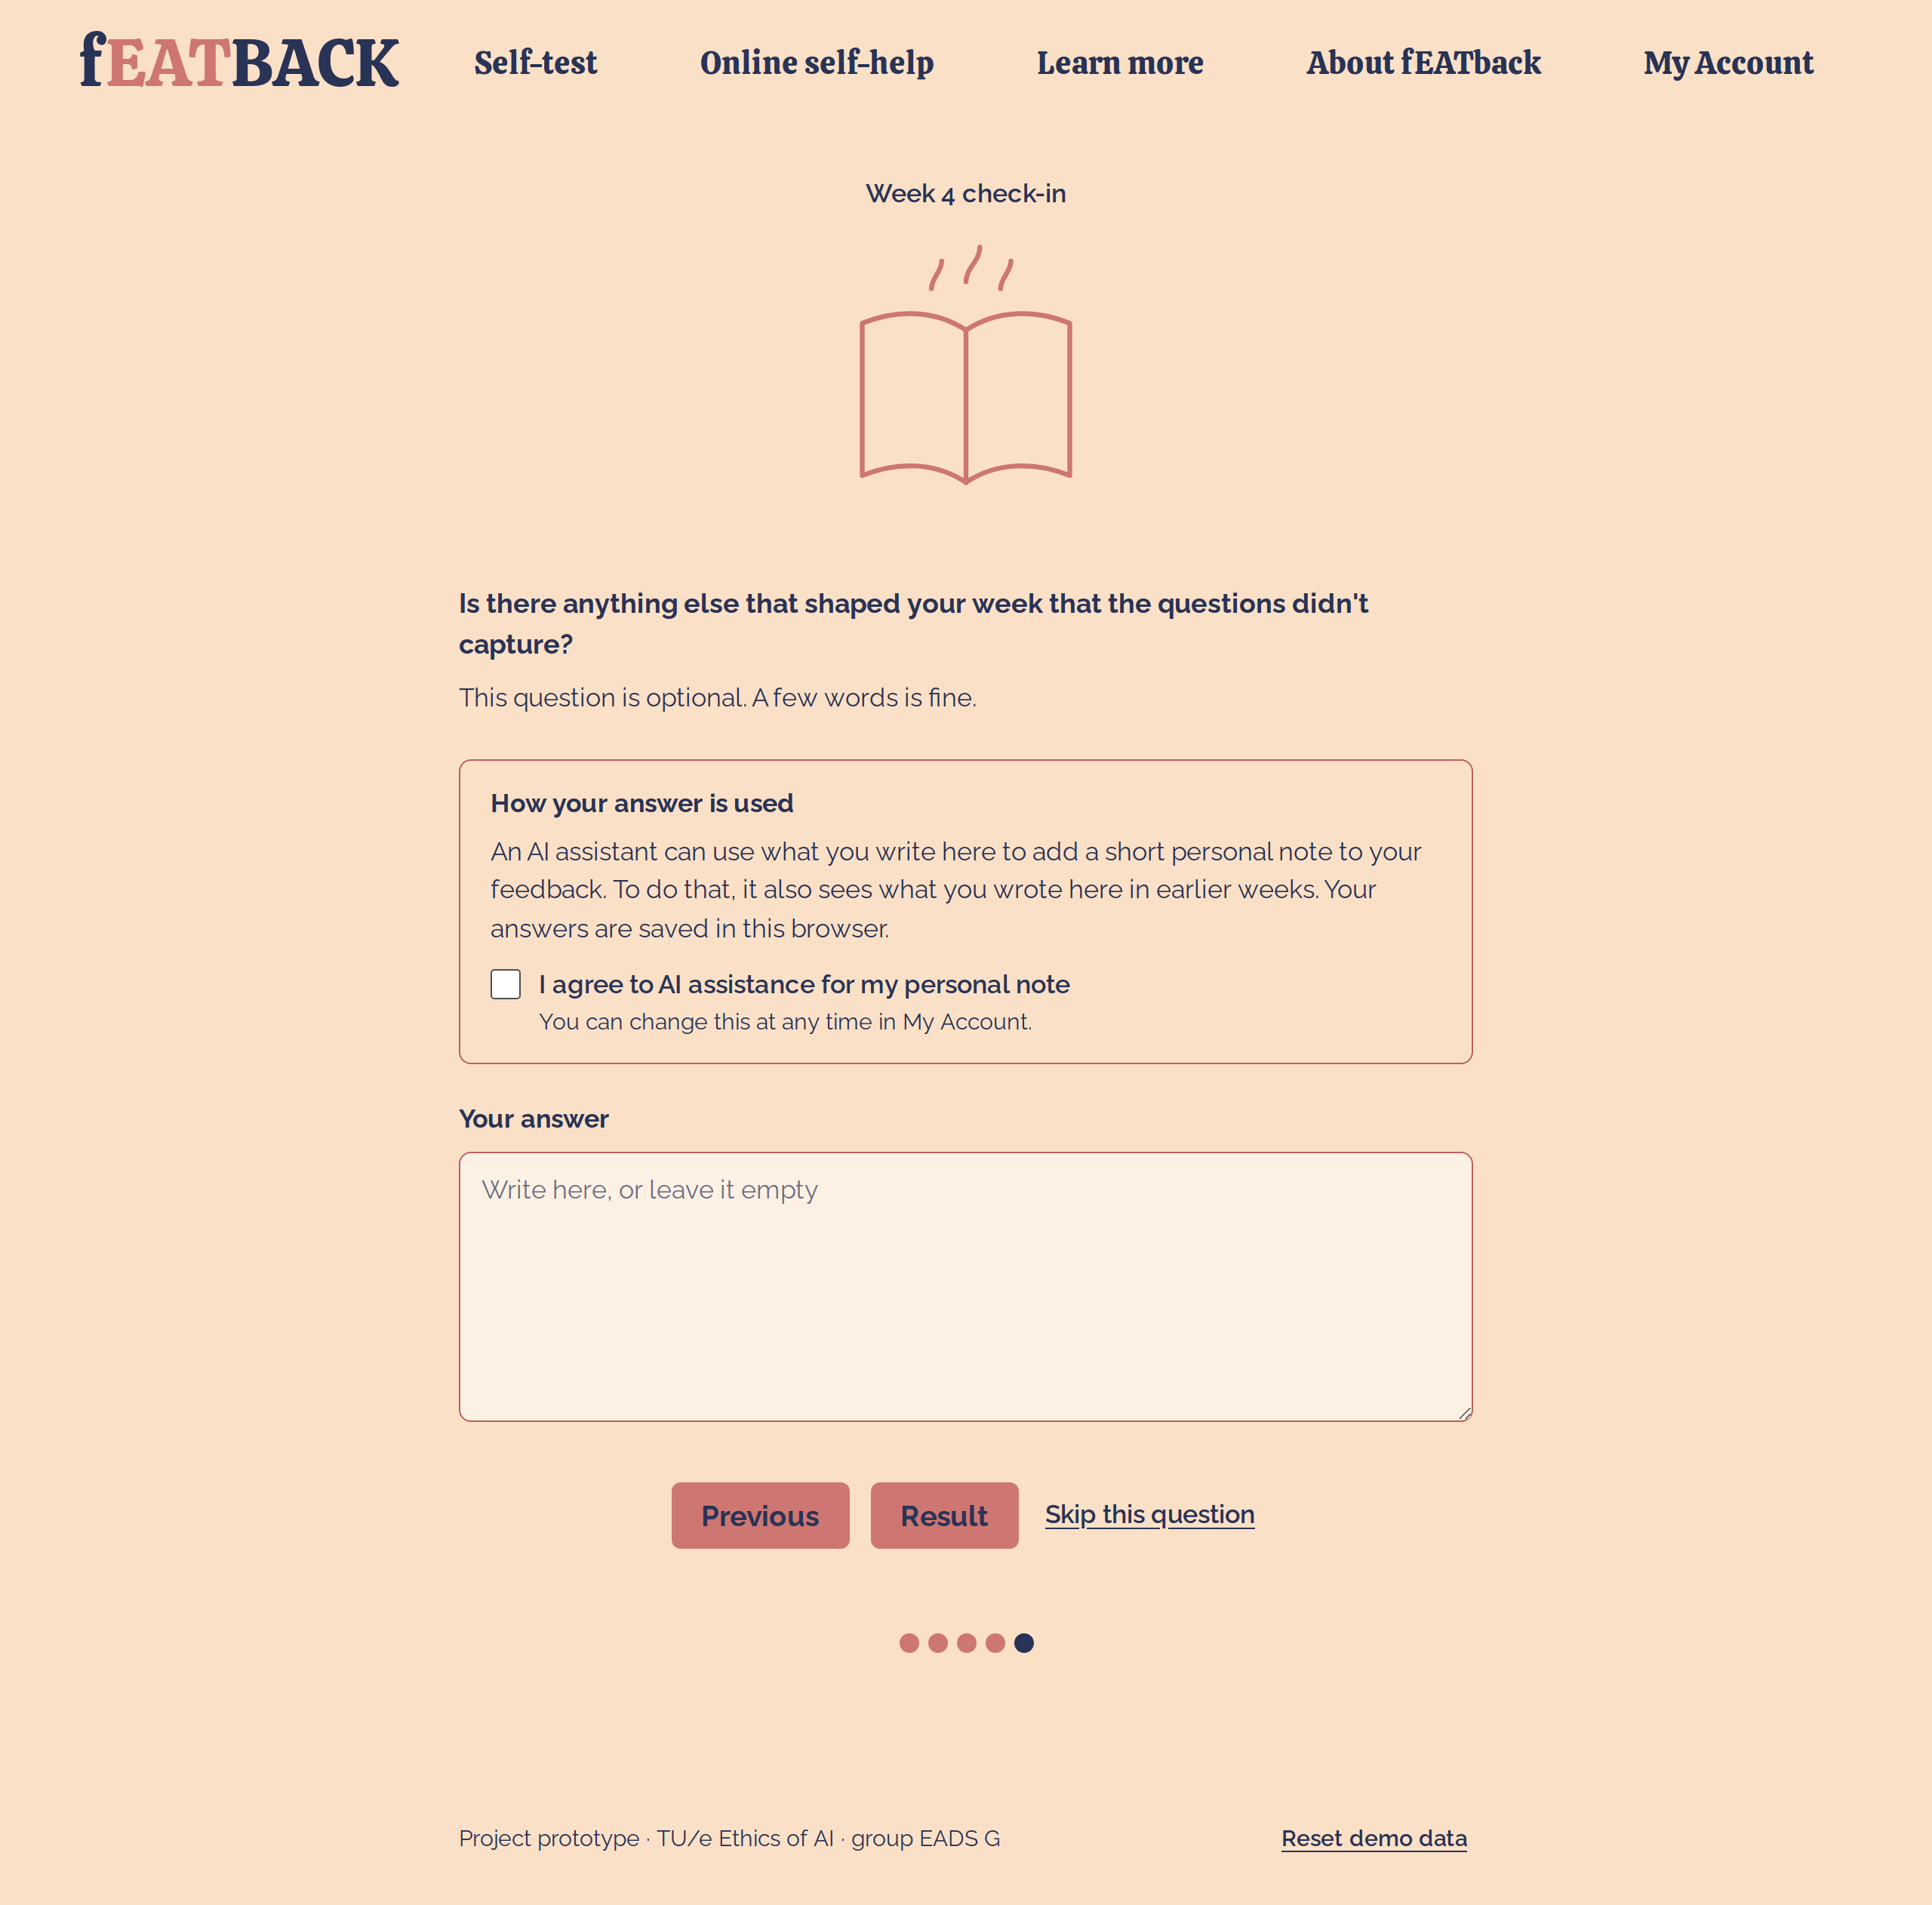
\includegraphics[width=\linewidth, trim=590 1087 590 760, clip]{q5_unticked.png}};
  \begin{scope}[x={(s.south east)}, y={(s.north west)}]
    \callout{0.979}{0.637}{1}
  \end{scope}
\end{tikzpicture}
\par\vspace{4mm}
\paneltitle{b}{Her answer and the result}
\begin{tikzpicture}
  \node[shot] (s) at (0,0) {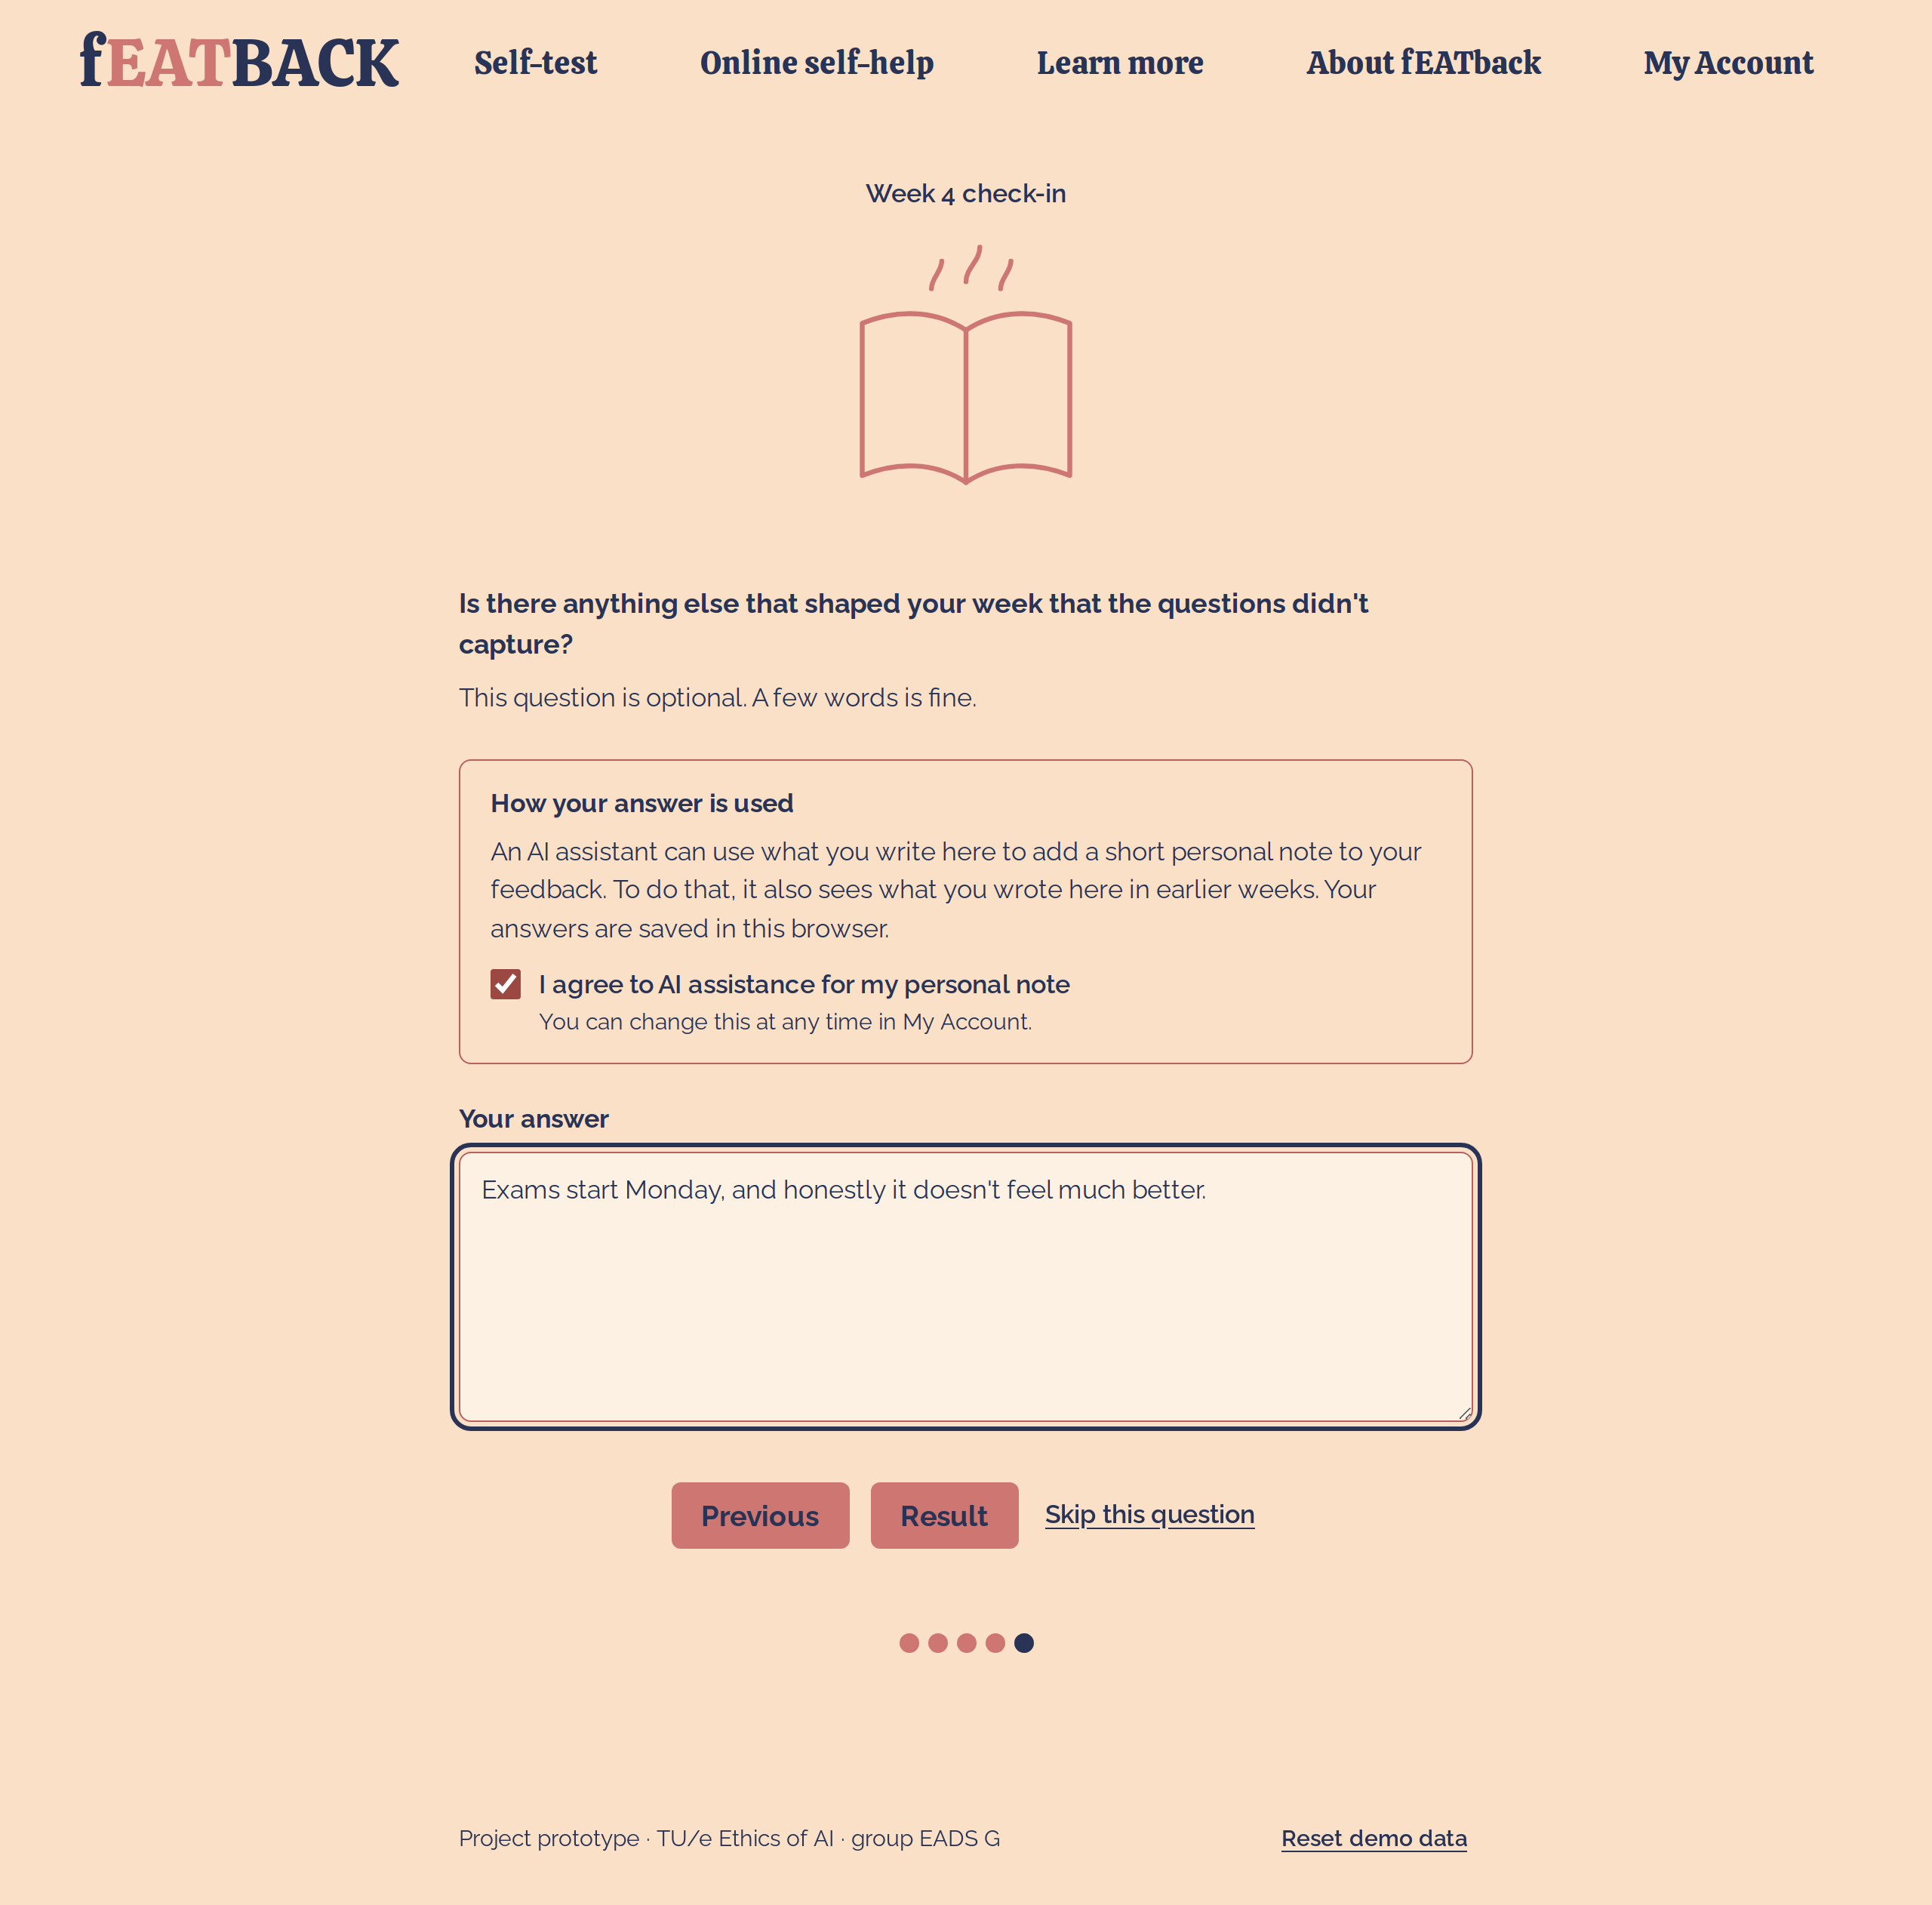
\includegraphics[width=\linewidth, trim=590 613 590 1440, clip]{q5_screen.png}};
  \begin{scope}[x={(s.south east)}, y={(s.north west)}]
    \callout{0.979}{0.817}{2}
  \end{scope}
\end{tikzpicture}
\par\vspace{1.5mm}
\begin{tikzpicture}
  \node[shot] (s) at (0,0) {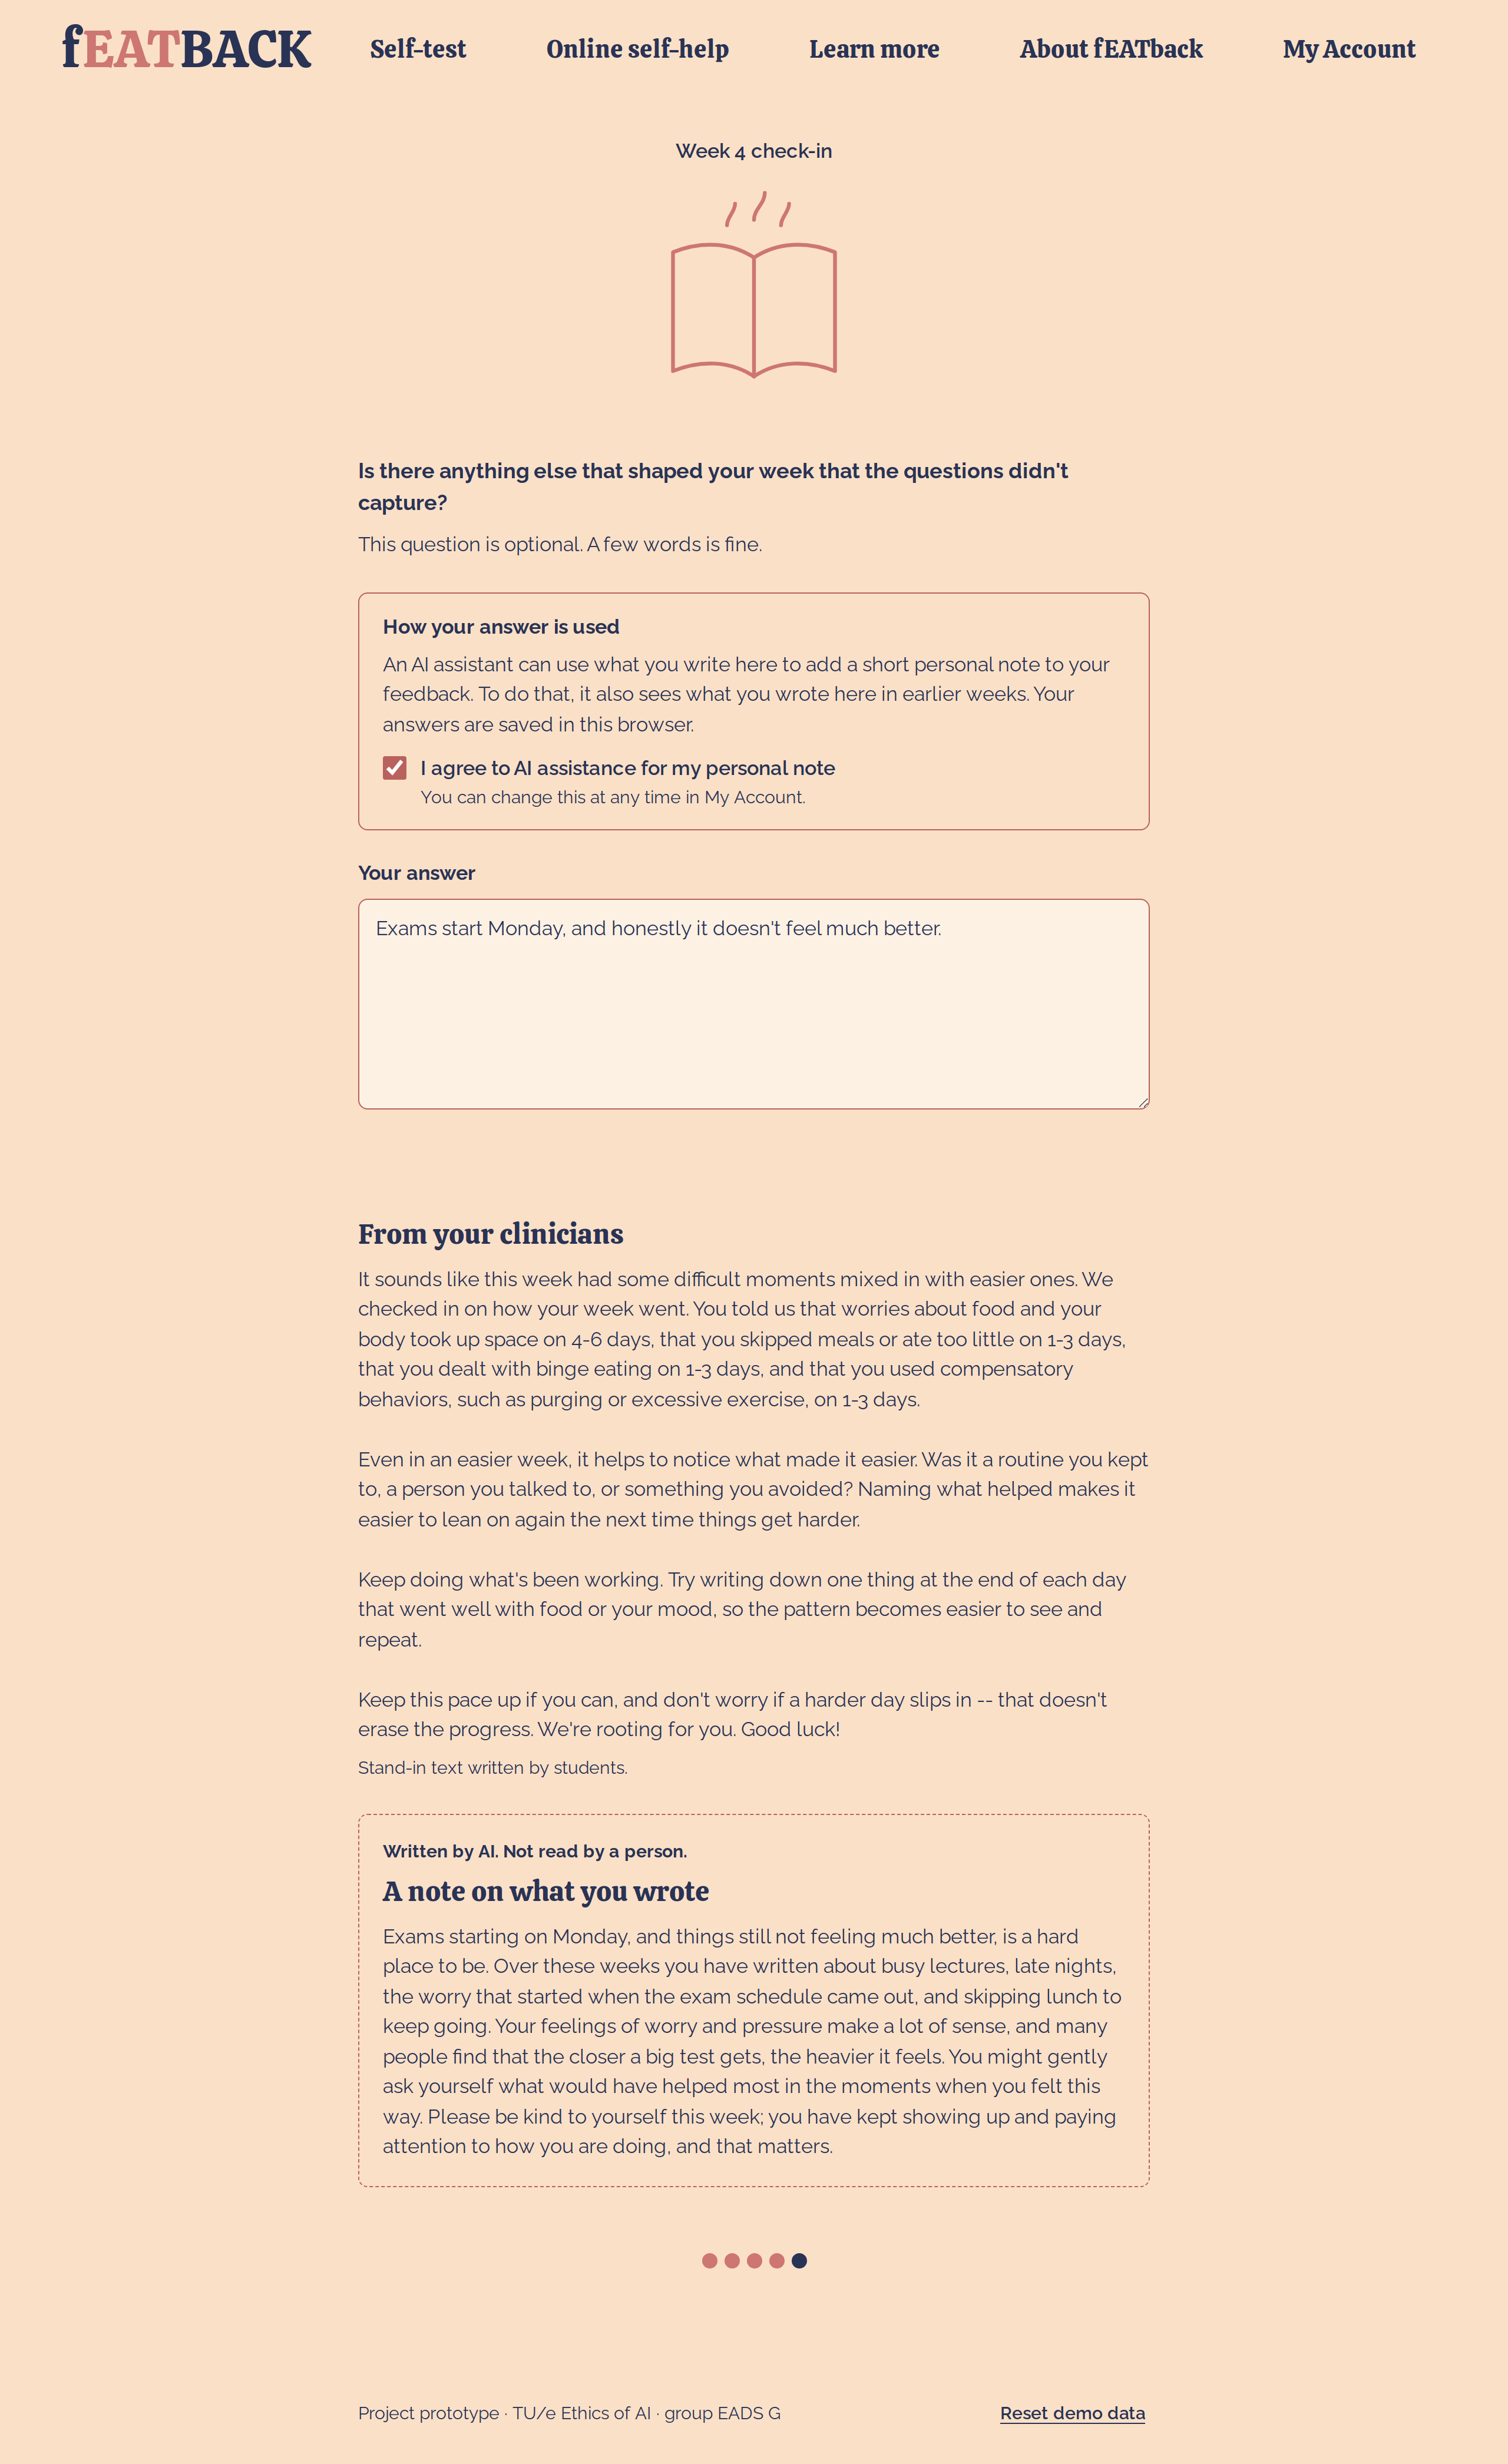
\includegraphics[width=\linewidth, trim=590 443 590 2046, clip]{result_screen.png}};
  \begin{scope}[x={(s.south east)}, y={(s.north west)}]
    \callout{0.979}{0.983}{3}
    \callout{0.979}{0.390}{4}
  \end{scope}
\end{tikzpicture}
\end{minipage}%
\hfill
% ============ Right column: other weeks and edge cases ============
\begin{minipage}[t]{0.47\textwidth}
\colhead{Week 5 and when something goes wrong}
\paneltitle{c}{Week 5, where the note looks back}
\begin{tikzpicture}
  \node[shot] (s) at (0,0) {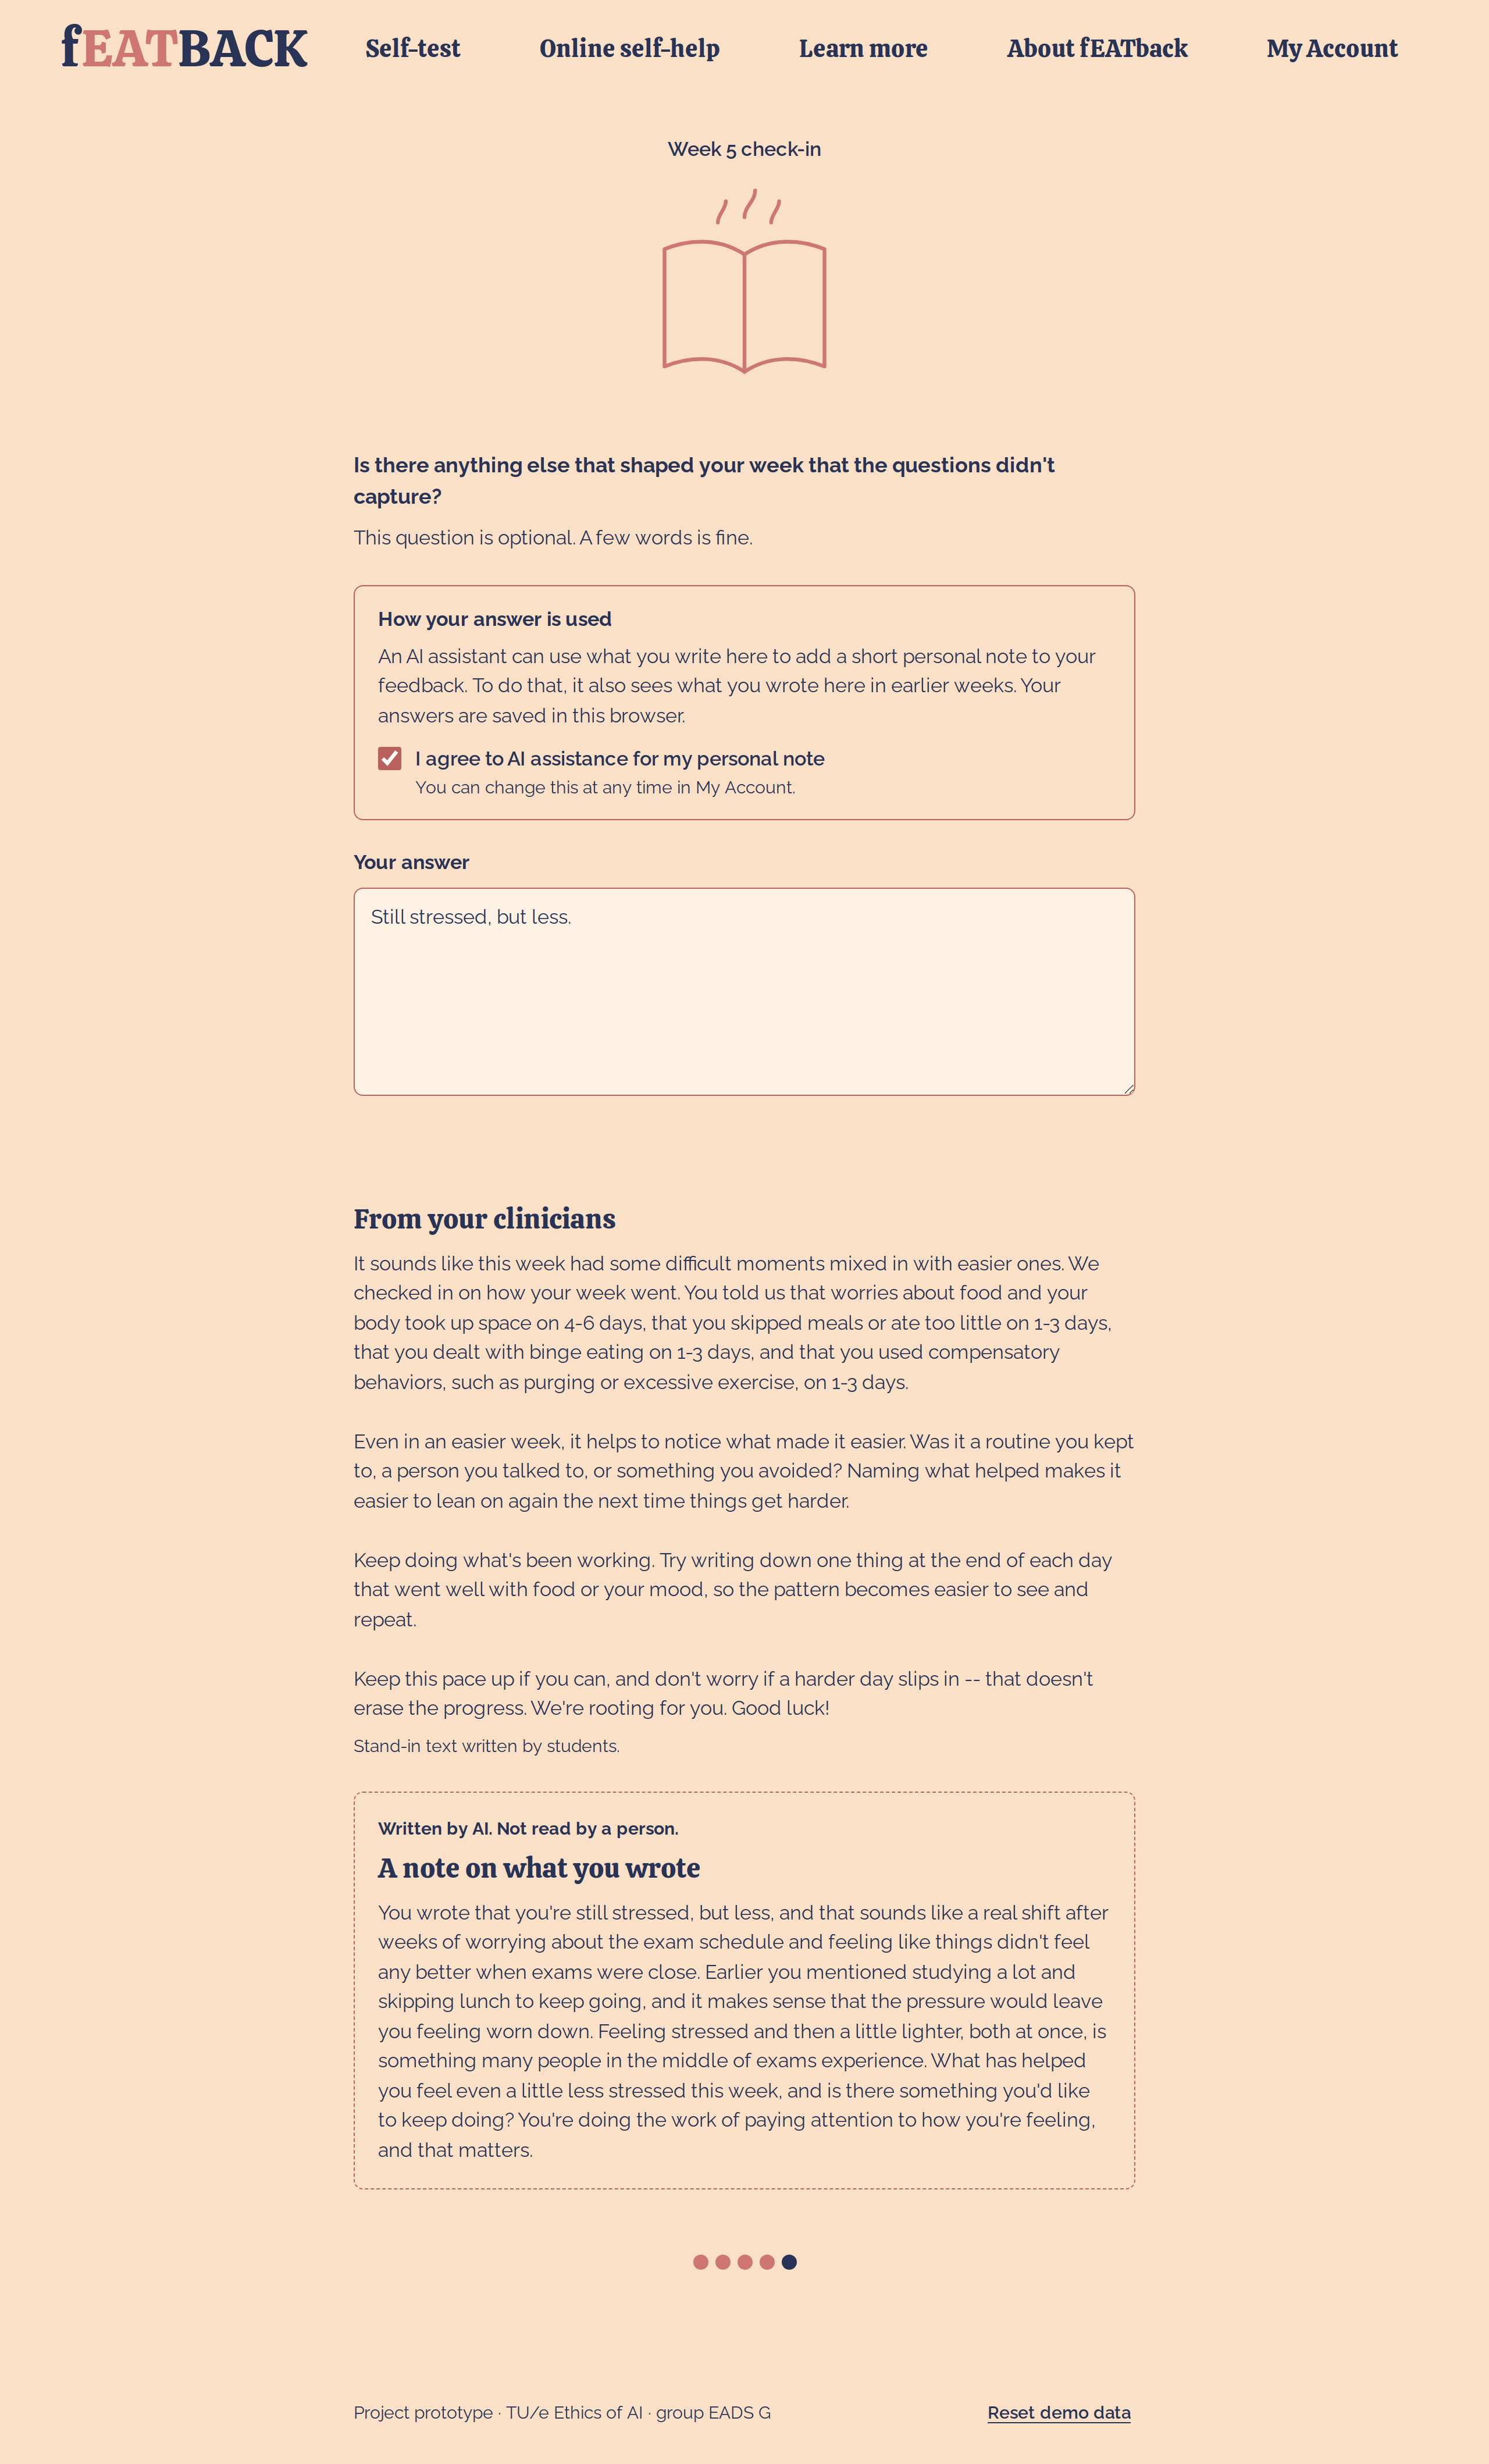
\includegraphics[width=\linewidth, trim=590 2325 590 1440, clip]{result_week5.png}};
\end{tikzpicture}
\par\vspace{1.5mm}
\begin{tikzpicture}
  \node[shot] (s) at (0,0) {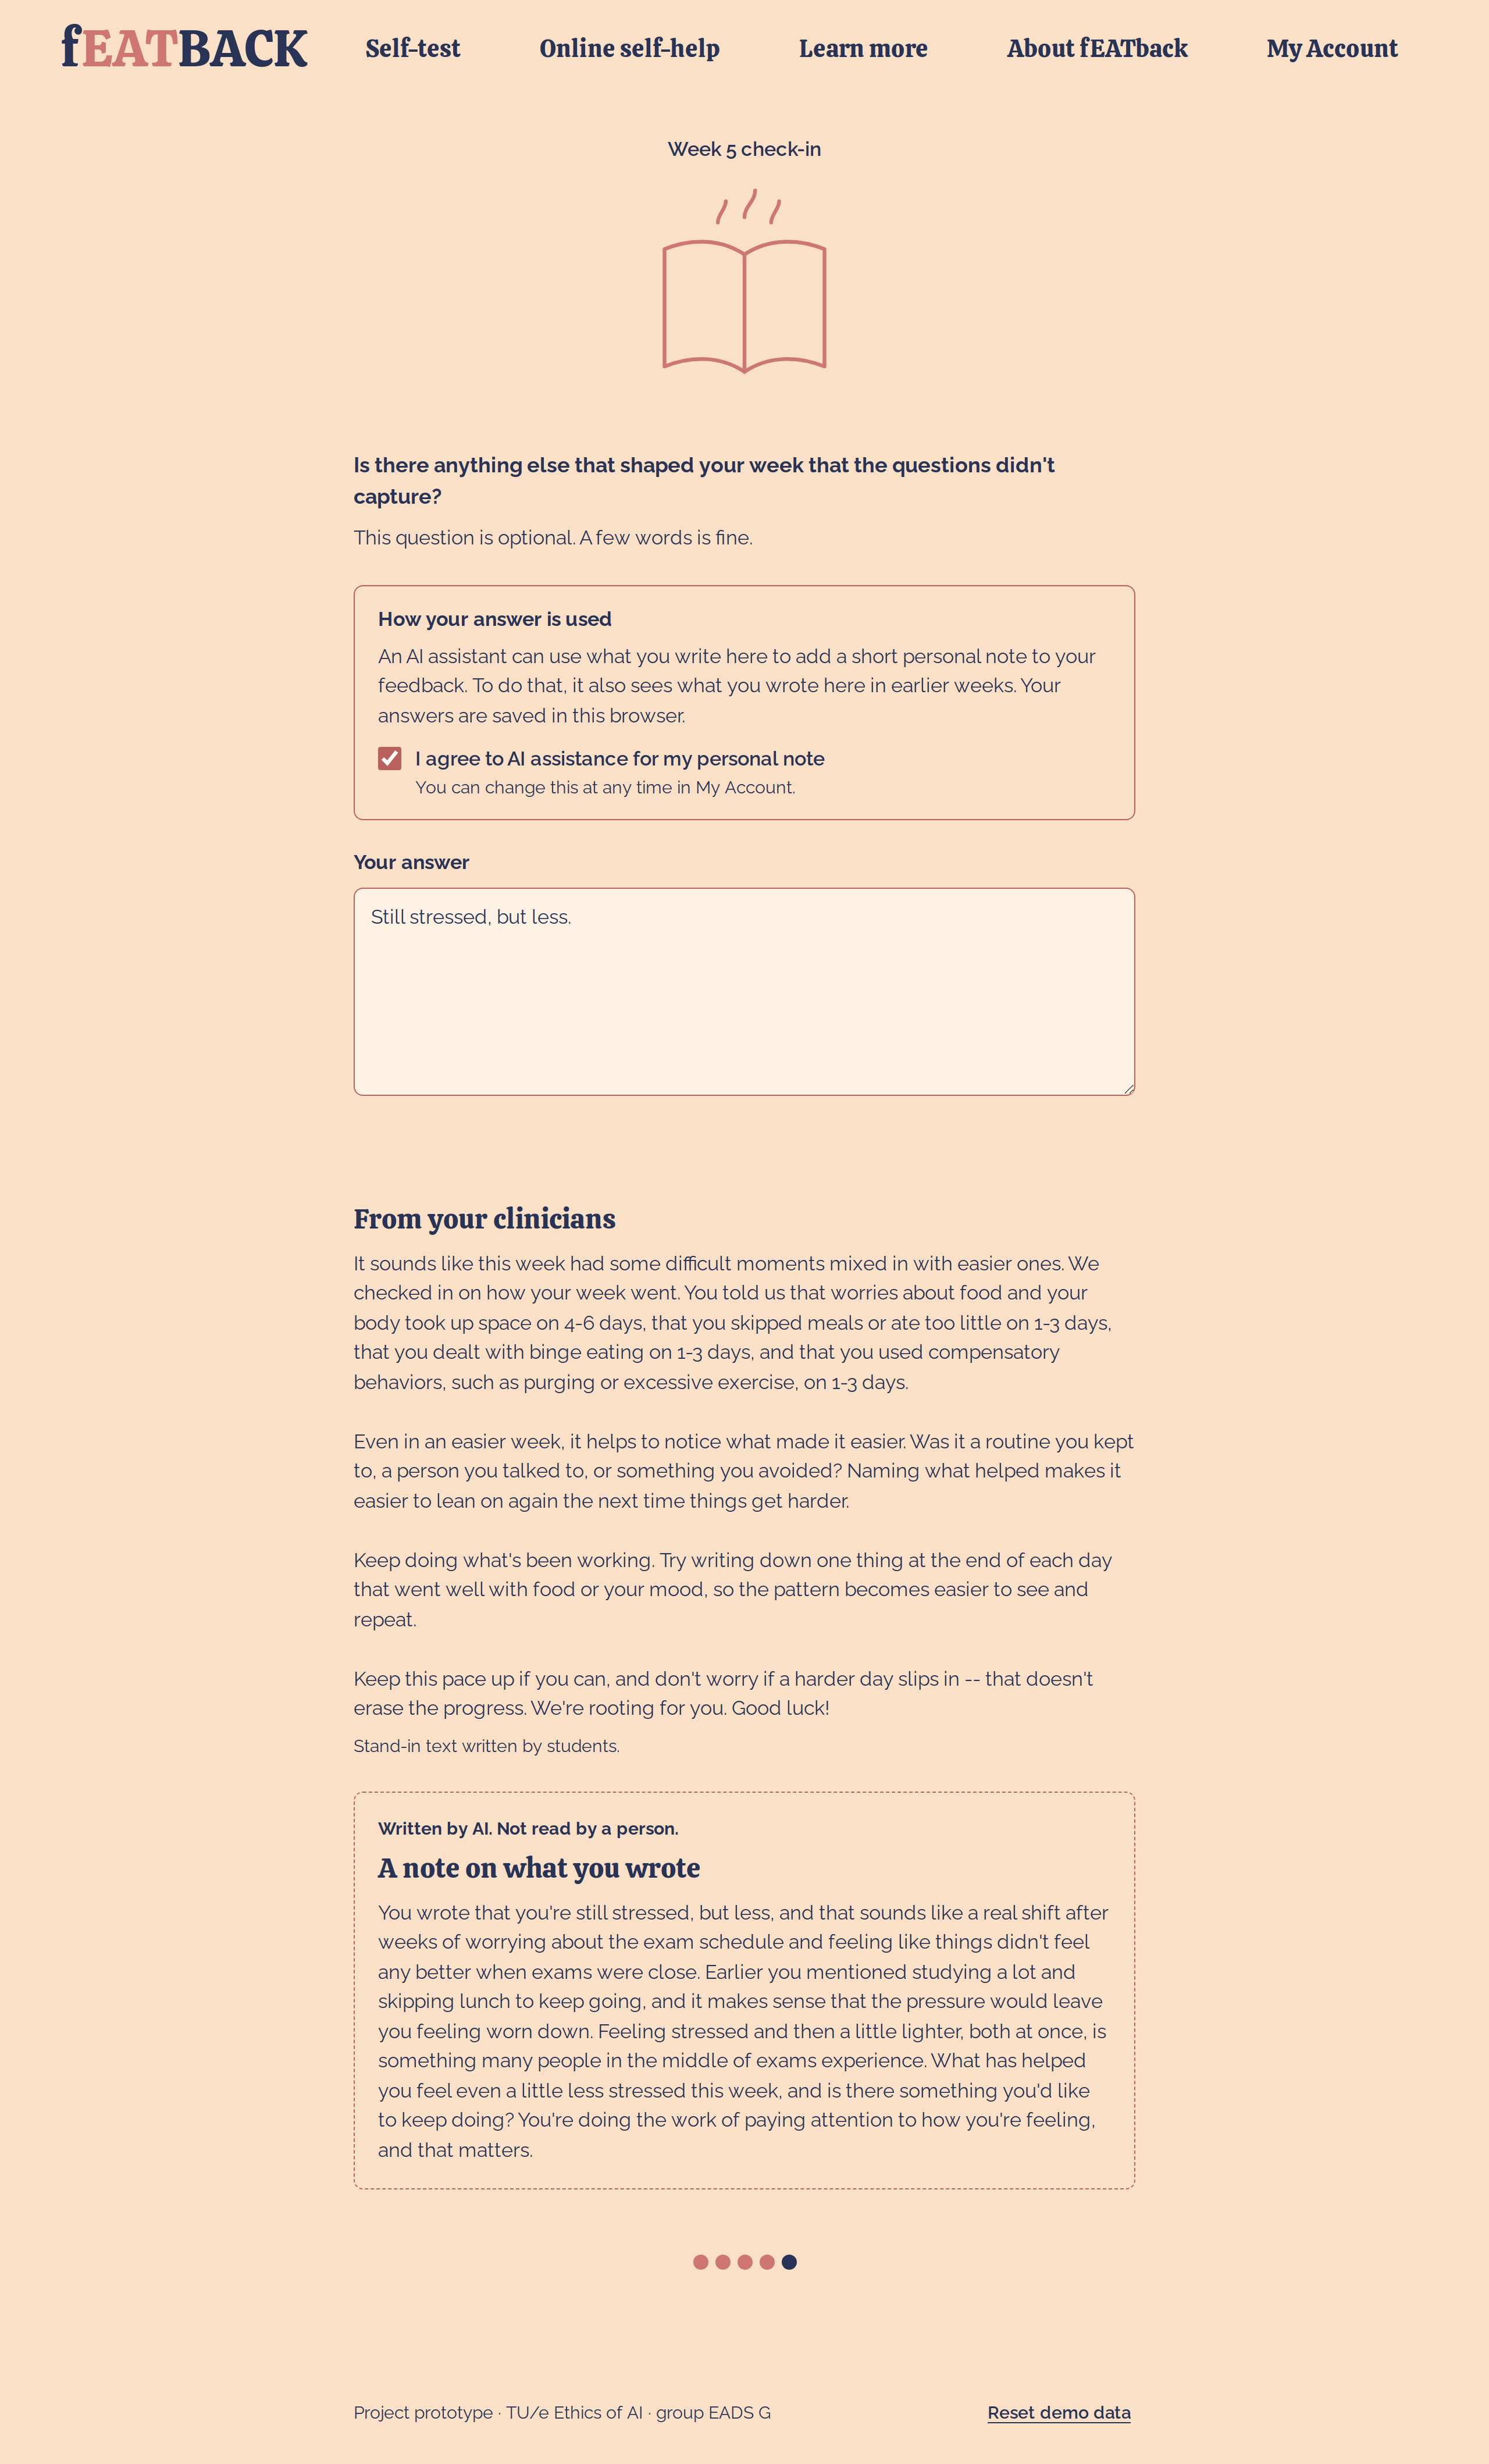
\includegraphics[width=\linewidth, trim=590 445 590 3052, clip]{result_week5.png}};
\end{tikzpicture}
\par\vspace{4mm}
\paneltitle{d}{Model off or note rejected}
\begin{tikzpicture}
  \node[shot] (s) at (0,0) {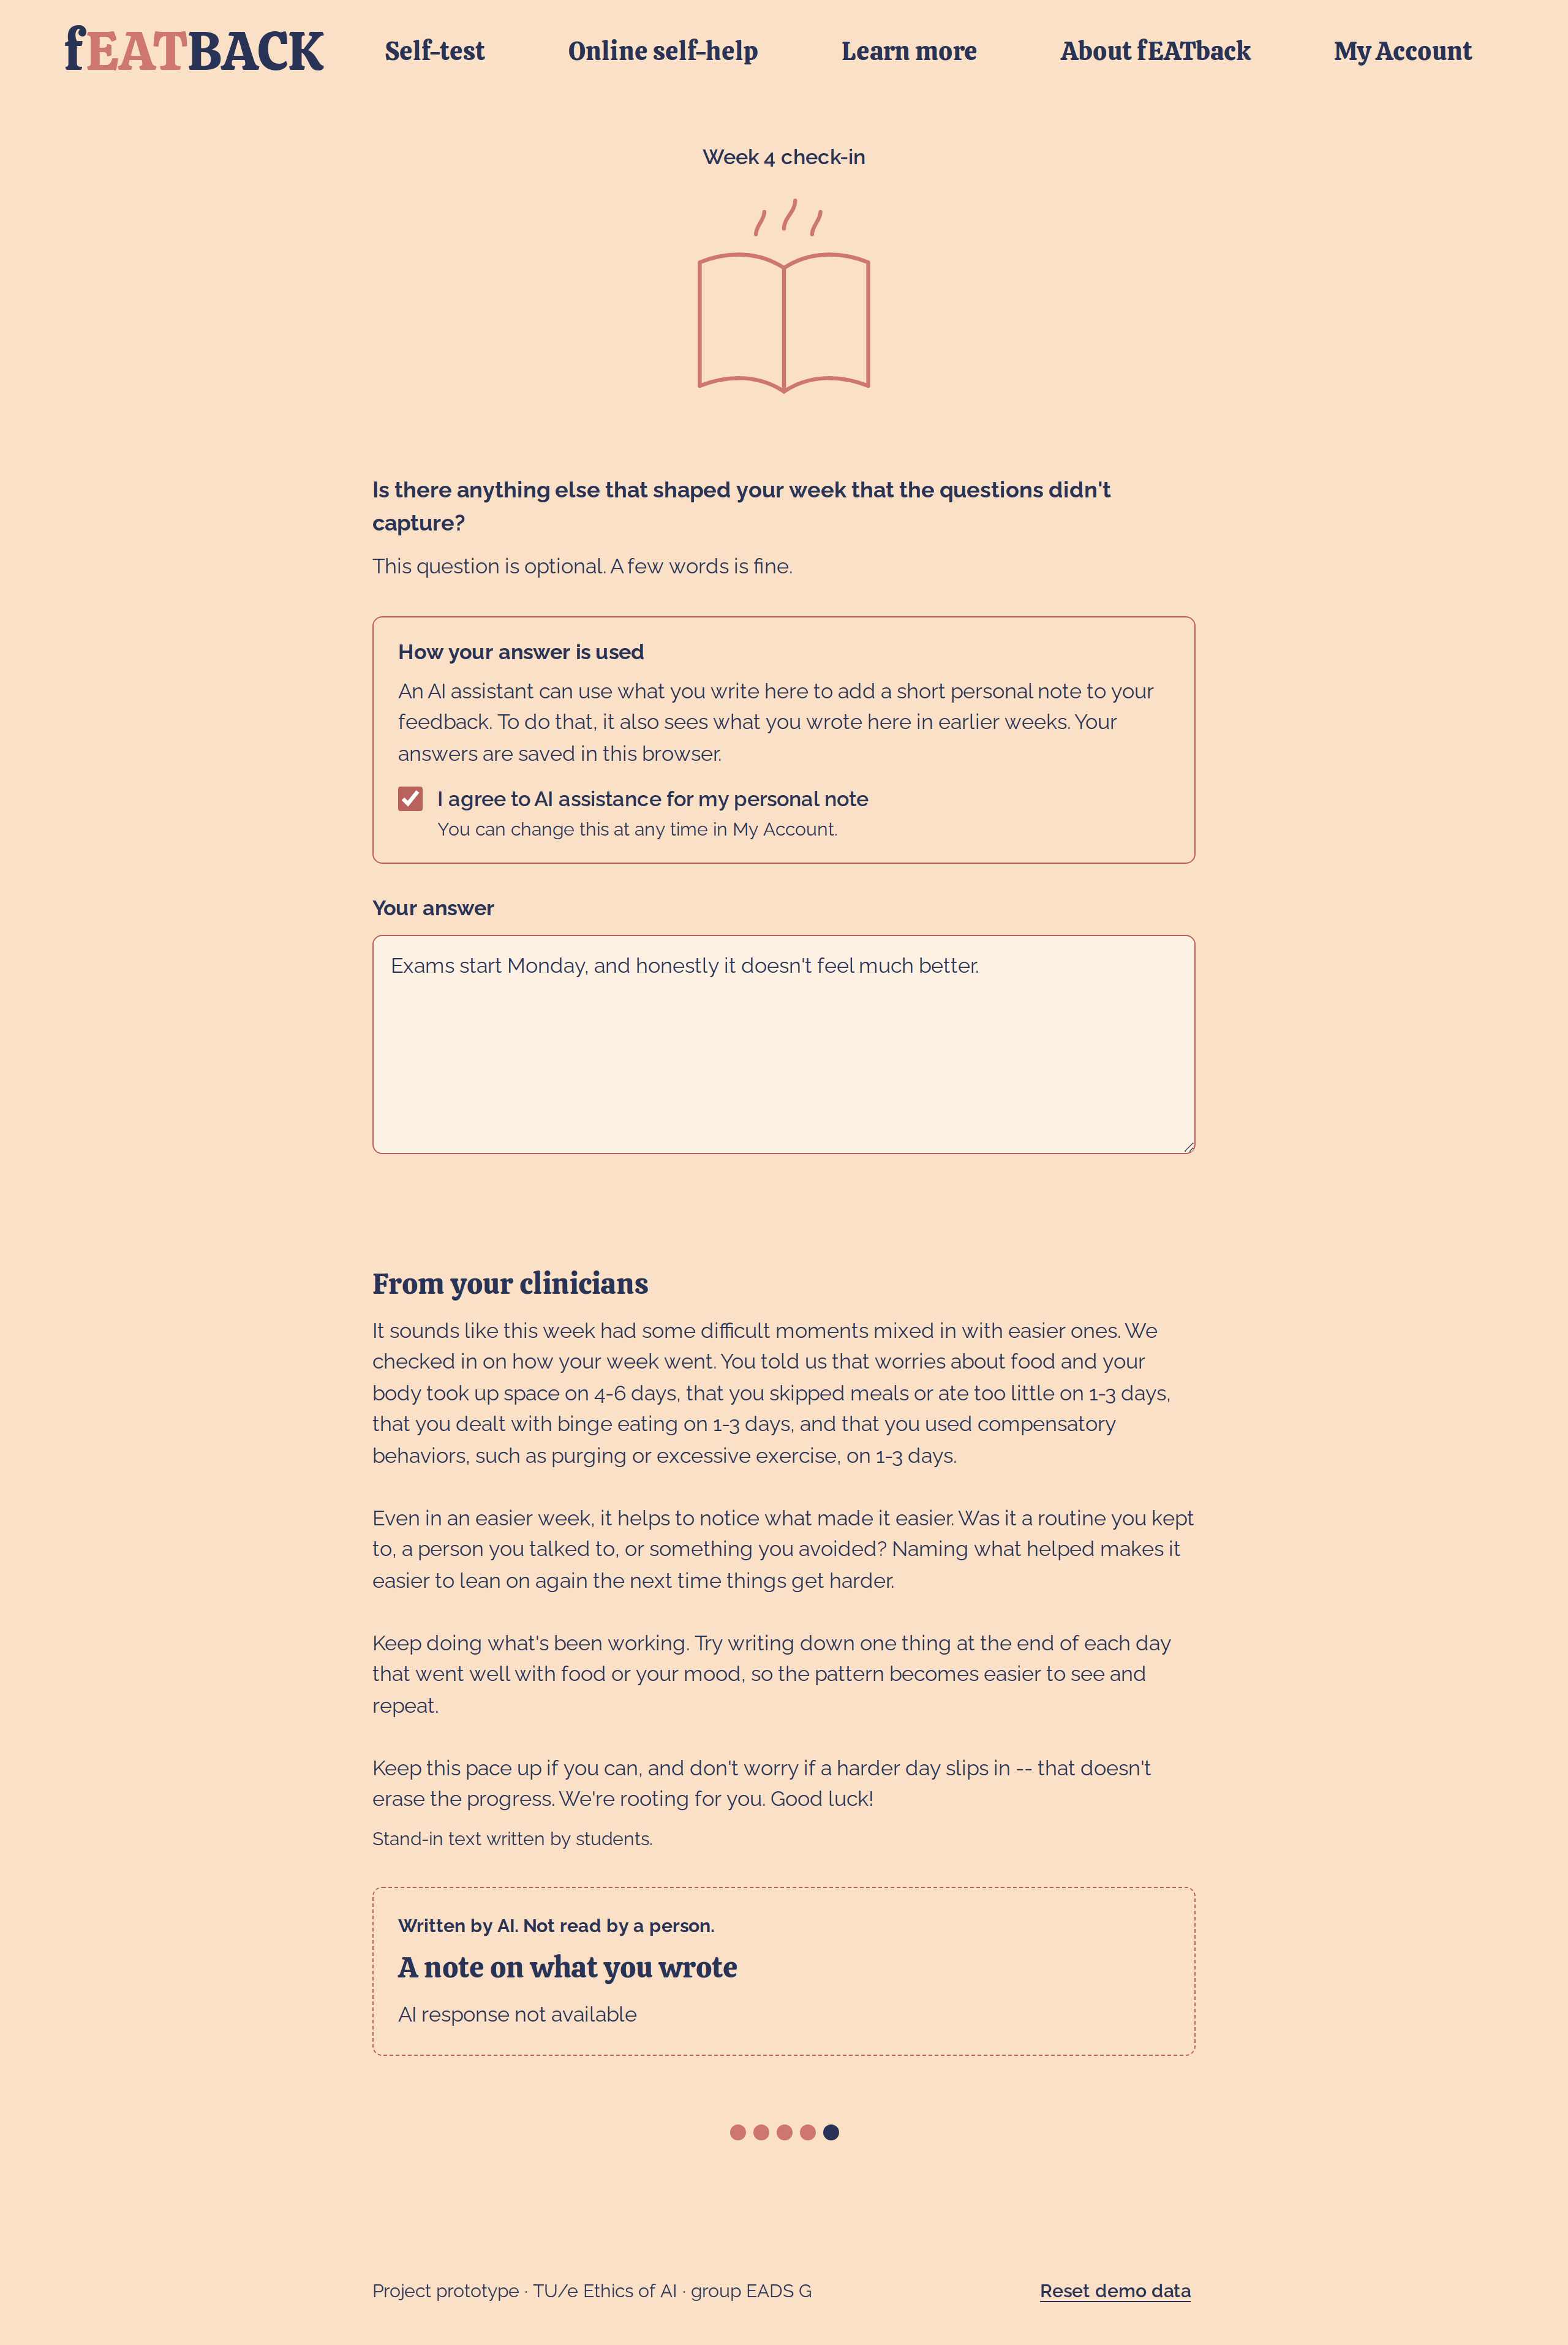
\includegraphics[width=\linewidth, trim=590 445 590 3052, clip]{fallback.png}};
  \begin{scope}[x={(s.south east)}, y={(s.north west)}]
    \callout{0.979}{0.915}{5}
  \end{scope}
\end{tikzpicture}
\par\vspace{4mm}
\paneltitle{e}{An answer with signs of acute risk}
\begin{tikzpicture}
  \node[shot] (s) at (0,0) {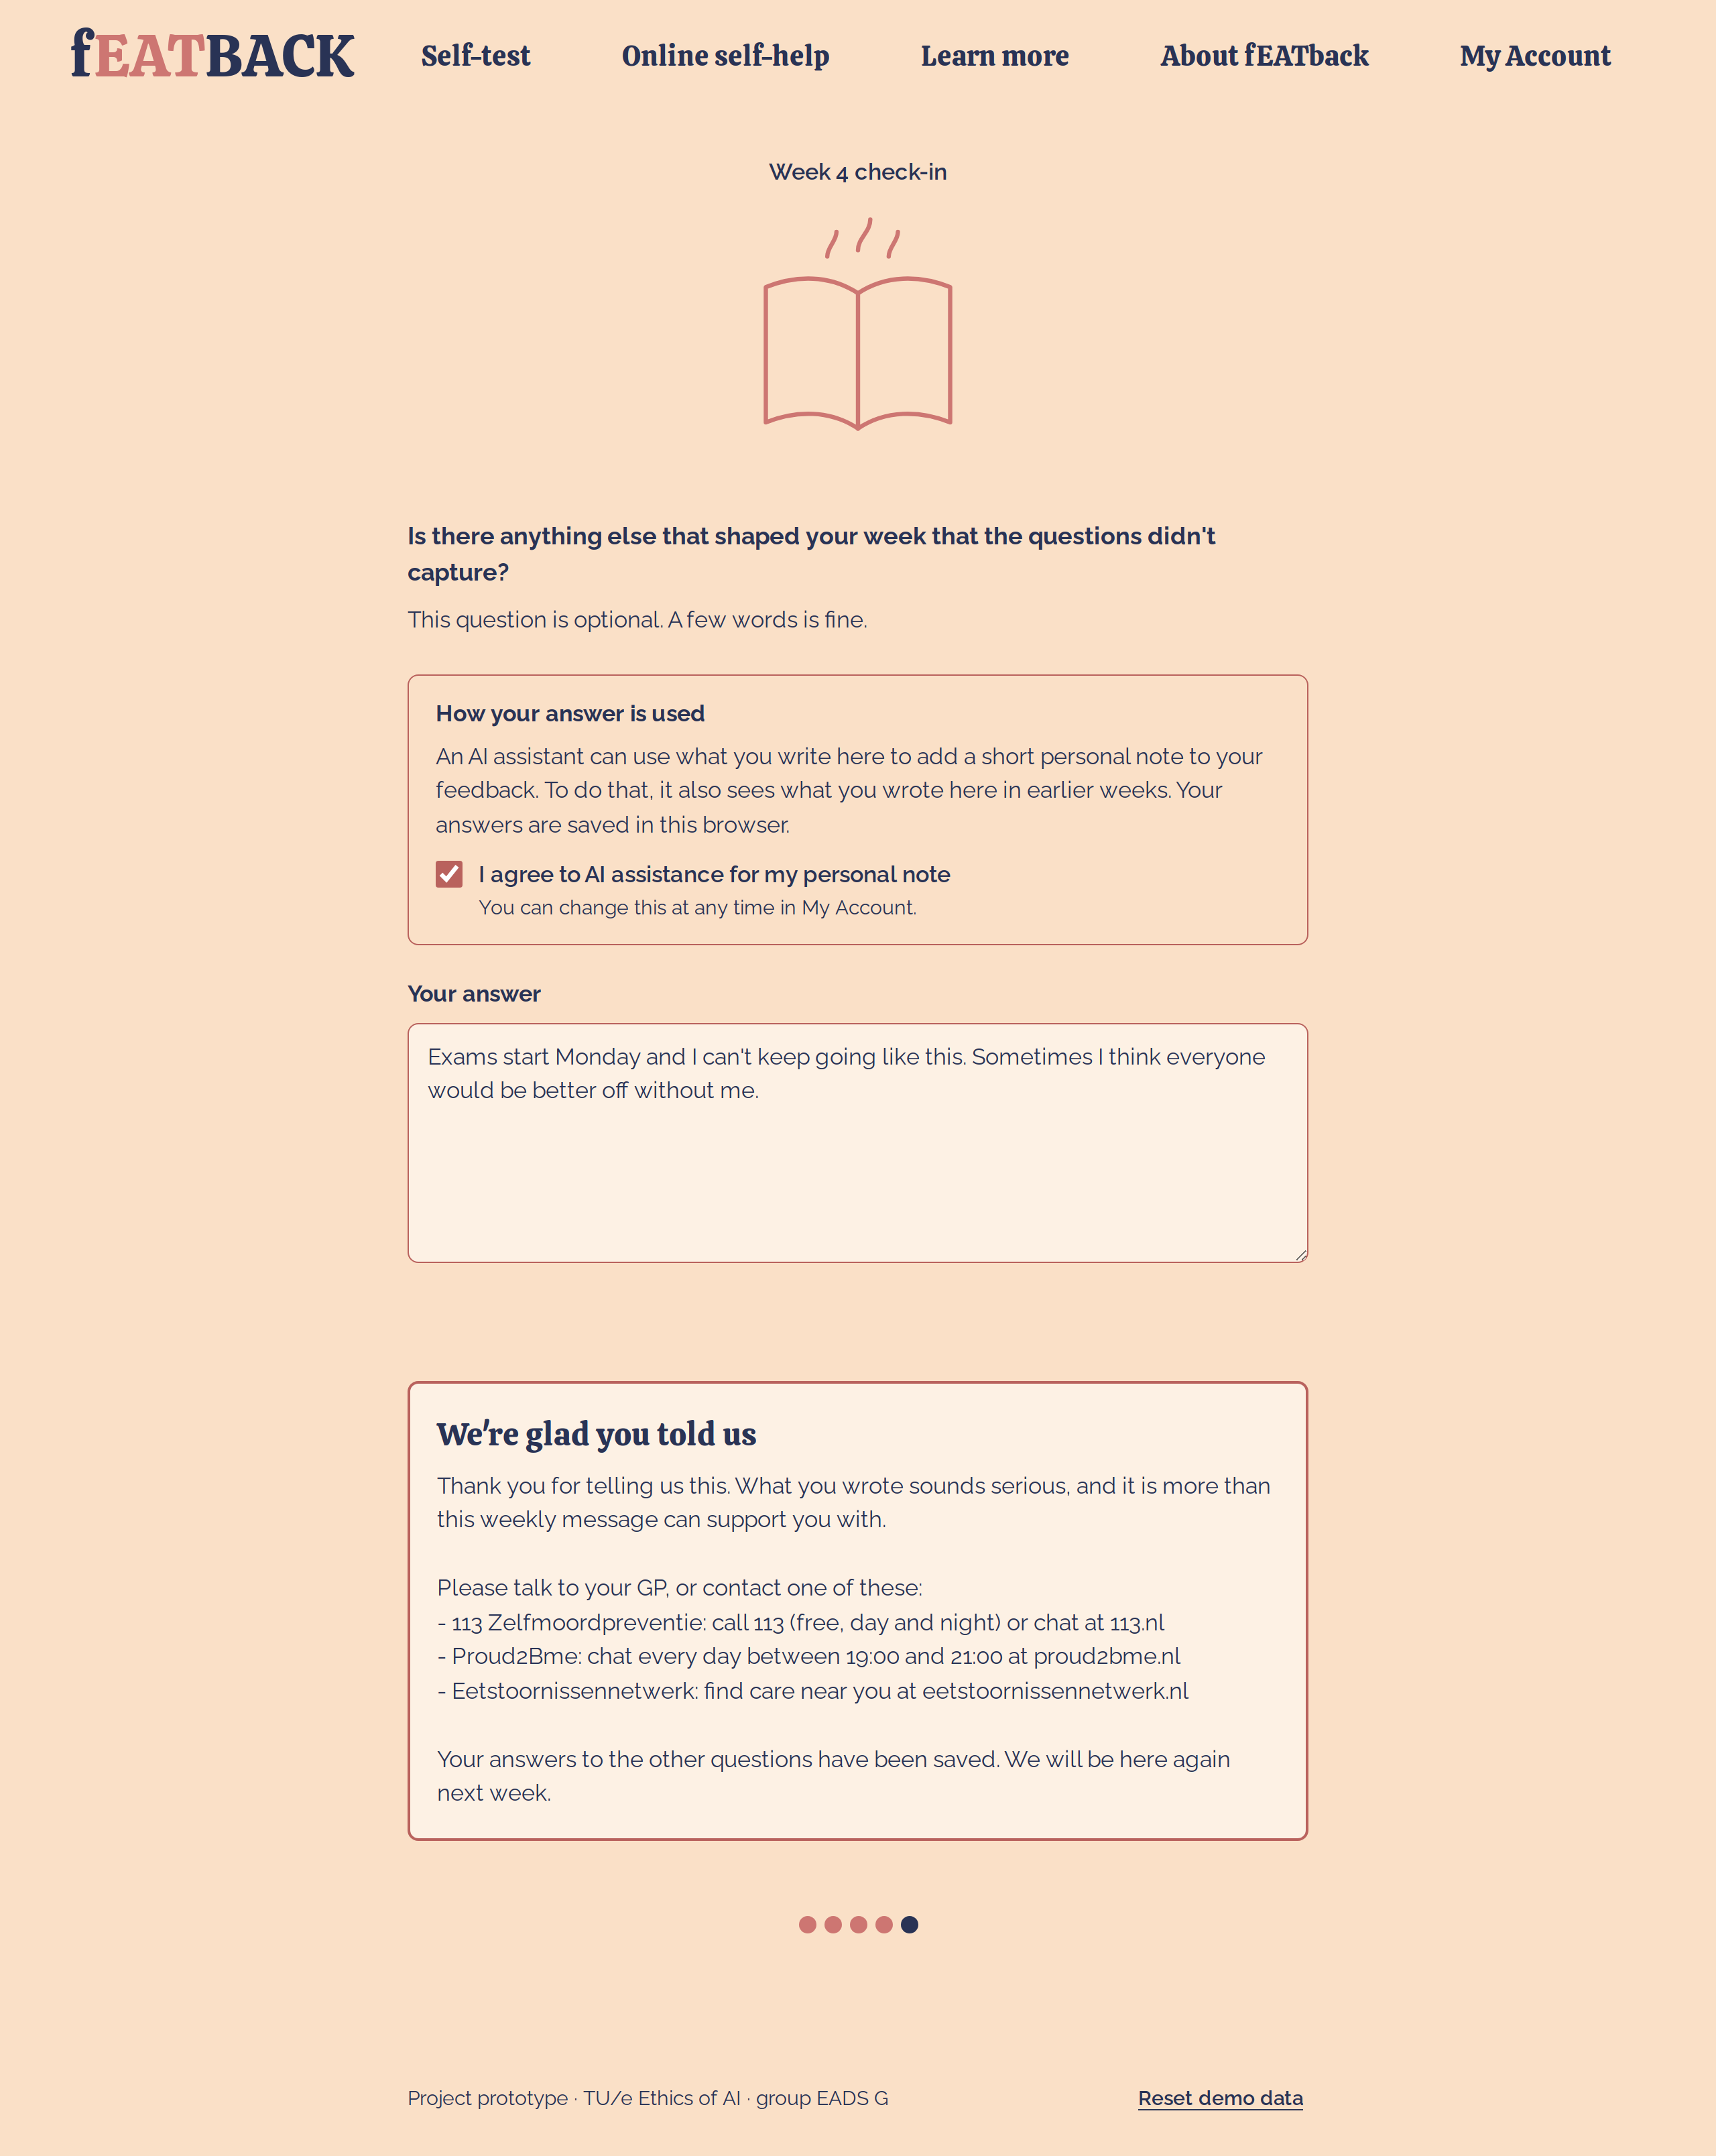
\includegraphics[width=\linewidth, trim=590 1305 590 1440, clip]{acute.png}};
\end{tikzpicture}
\par\vspace{1.5mm}
\begin{tikzpicture}
  \node[shot] (s) at (0,0) {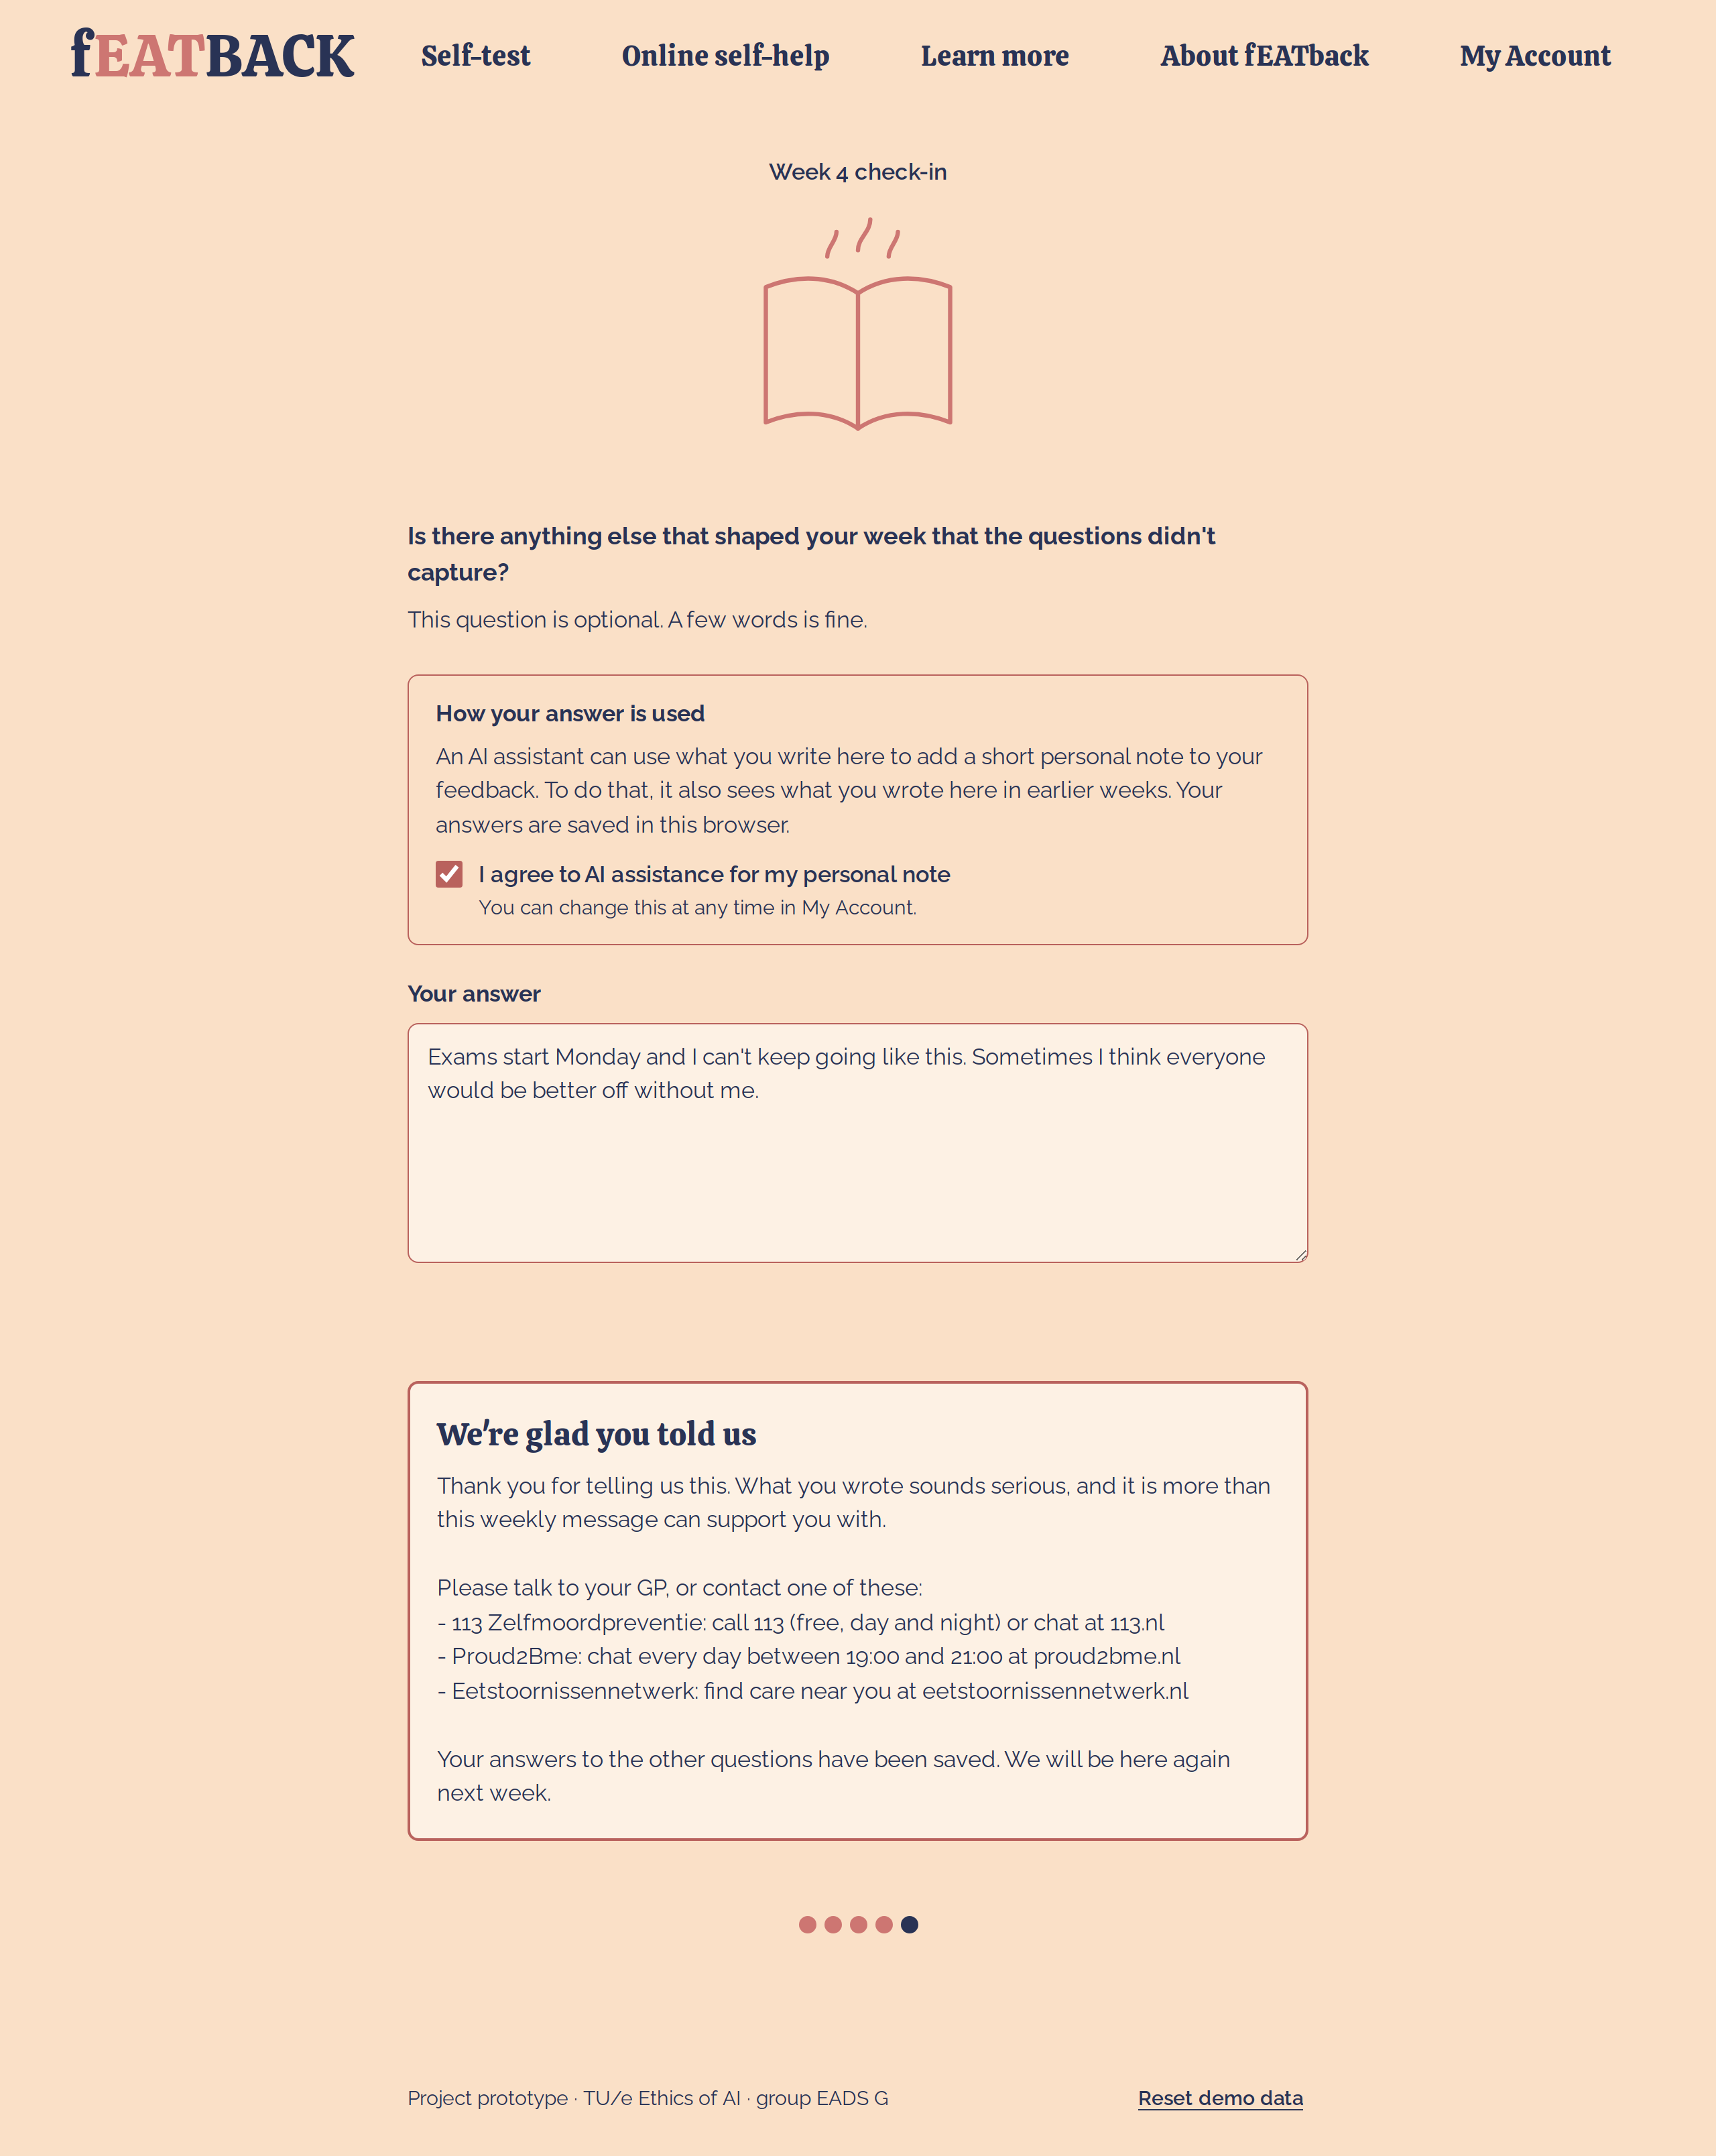
\includegraphics[width=\linewidth, trim=590 443 590 2032, clip]{acute.png}};
  \begin{scope}[x={(s.south east)}, y={(s.north west)}]
    \callout{0.979}{0.962}{6}
  \end{scope}
\end{tikzpicture}
\end{minipage}

\vspace{5mm}
% ---- Key: one entry per callout, aligned with the two columns ----
\newcommand{\keyline}[2]{\key{#1}\hspace{2mm}#2\par\vspace{1.2mm}}
{\footnotesize\sffamily
\begin{minipage}[t]{0.47\textwidth}
\keyline{1}{Consent box starts unticked (part 3)}
\keyline{2}{Answer stored for the trend (part 3)}
\keyline{3}{Stand-in bank message (part 1)}
\end{minipage}\hfill
\begin{minipage}[t]{0.47\textwidth}
\keyline{4}{Label on every AI note (part 2)}
\keyline{5}{Fixed fallback text we wrote (part 1)}
\keyline{6}{Gate takes the more severe label (part 1)}
\end{minipage}}

\vspace{2mm}
\caption{Maren's check-ins from Section~\ref{sec:narrative} as they appear on screen. Part numbers in the key
point to the Responsible Innovation statement. The AI notes in (b) and (c) are real
output from our fine-tuned writer model, run on 12 October 2026. The bank message, Maren
and her earlier answers are made up for the demo.}
\label{fig:mockup}
\end{figure}
.
% Needs tikz (loaded by todonotes in main.tex), graphicx and float.

% ---- Figure style ----------------------------------------------------------
\definecolor{fbnavy}{HTML}{283357}
\tikzset{
  shot/.style={anchor=south west, inner sep=0, draw=black!18, line width=0.4pt},
  callout/.style={circle, fill=fbnavy, draw=white, line width=0.9pt, text=white,
    font=\sffamily\bfseries\scriptsize, inner sep=0pt, minimum size=4.4mm}}
% Callouts sit on the right edge, level with the element they mark.
\newcommand{\callout}[3]{\node[callout, overlay] at (#1,#2) {#3};}
% Inline callout for the key
\newcommand{\key}[1]{\tikz[baseline=-0.6ex]\node[callout]{#1};}
% Panel title
\newcommand{\paneltitle}[2]{{\sffamily\footnotesize\color{fbnavy}\textbf{(#1)}~#2}\par\vspace{1mm}}
\newcommand{\colhead}[1]{{\sffamily\small\bfseries\color{fbnavy}#1}\par\vspace{0.5mm}{\color{black!25}\hrule height 0.4pt}\vspace{2mm}}

\begin{figure}[H]
\centering
% ============ Left column: week 4 ============
\begin{minipage}[t]{0.47\textwidth}
\colhead{Week 4}
\paneltitle{a}{Question 5, before she agrees}
\begin{tikzpicture}
  \node[shot] (s) at (0,0) {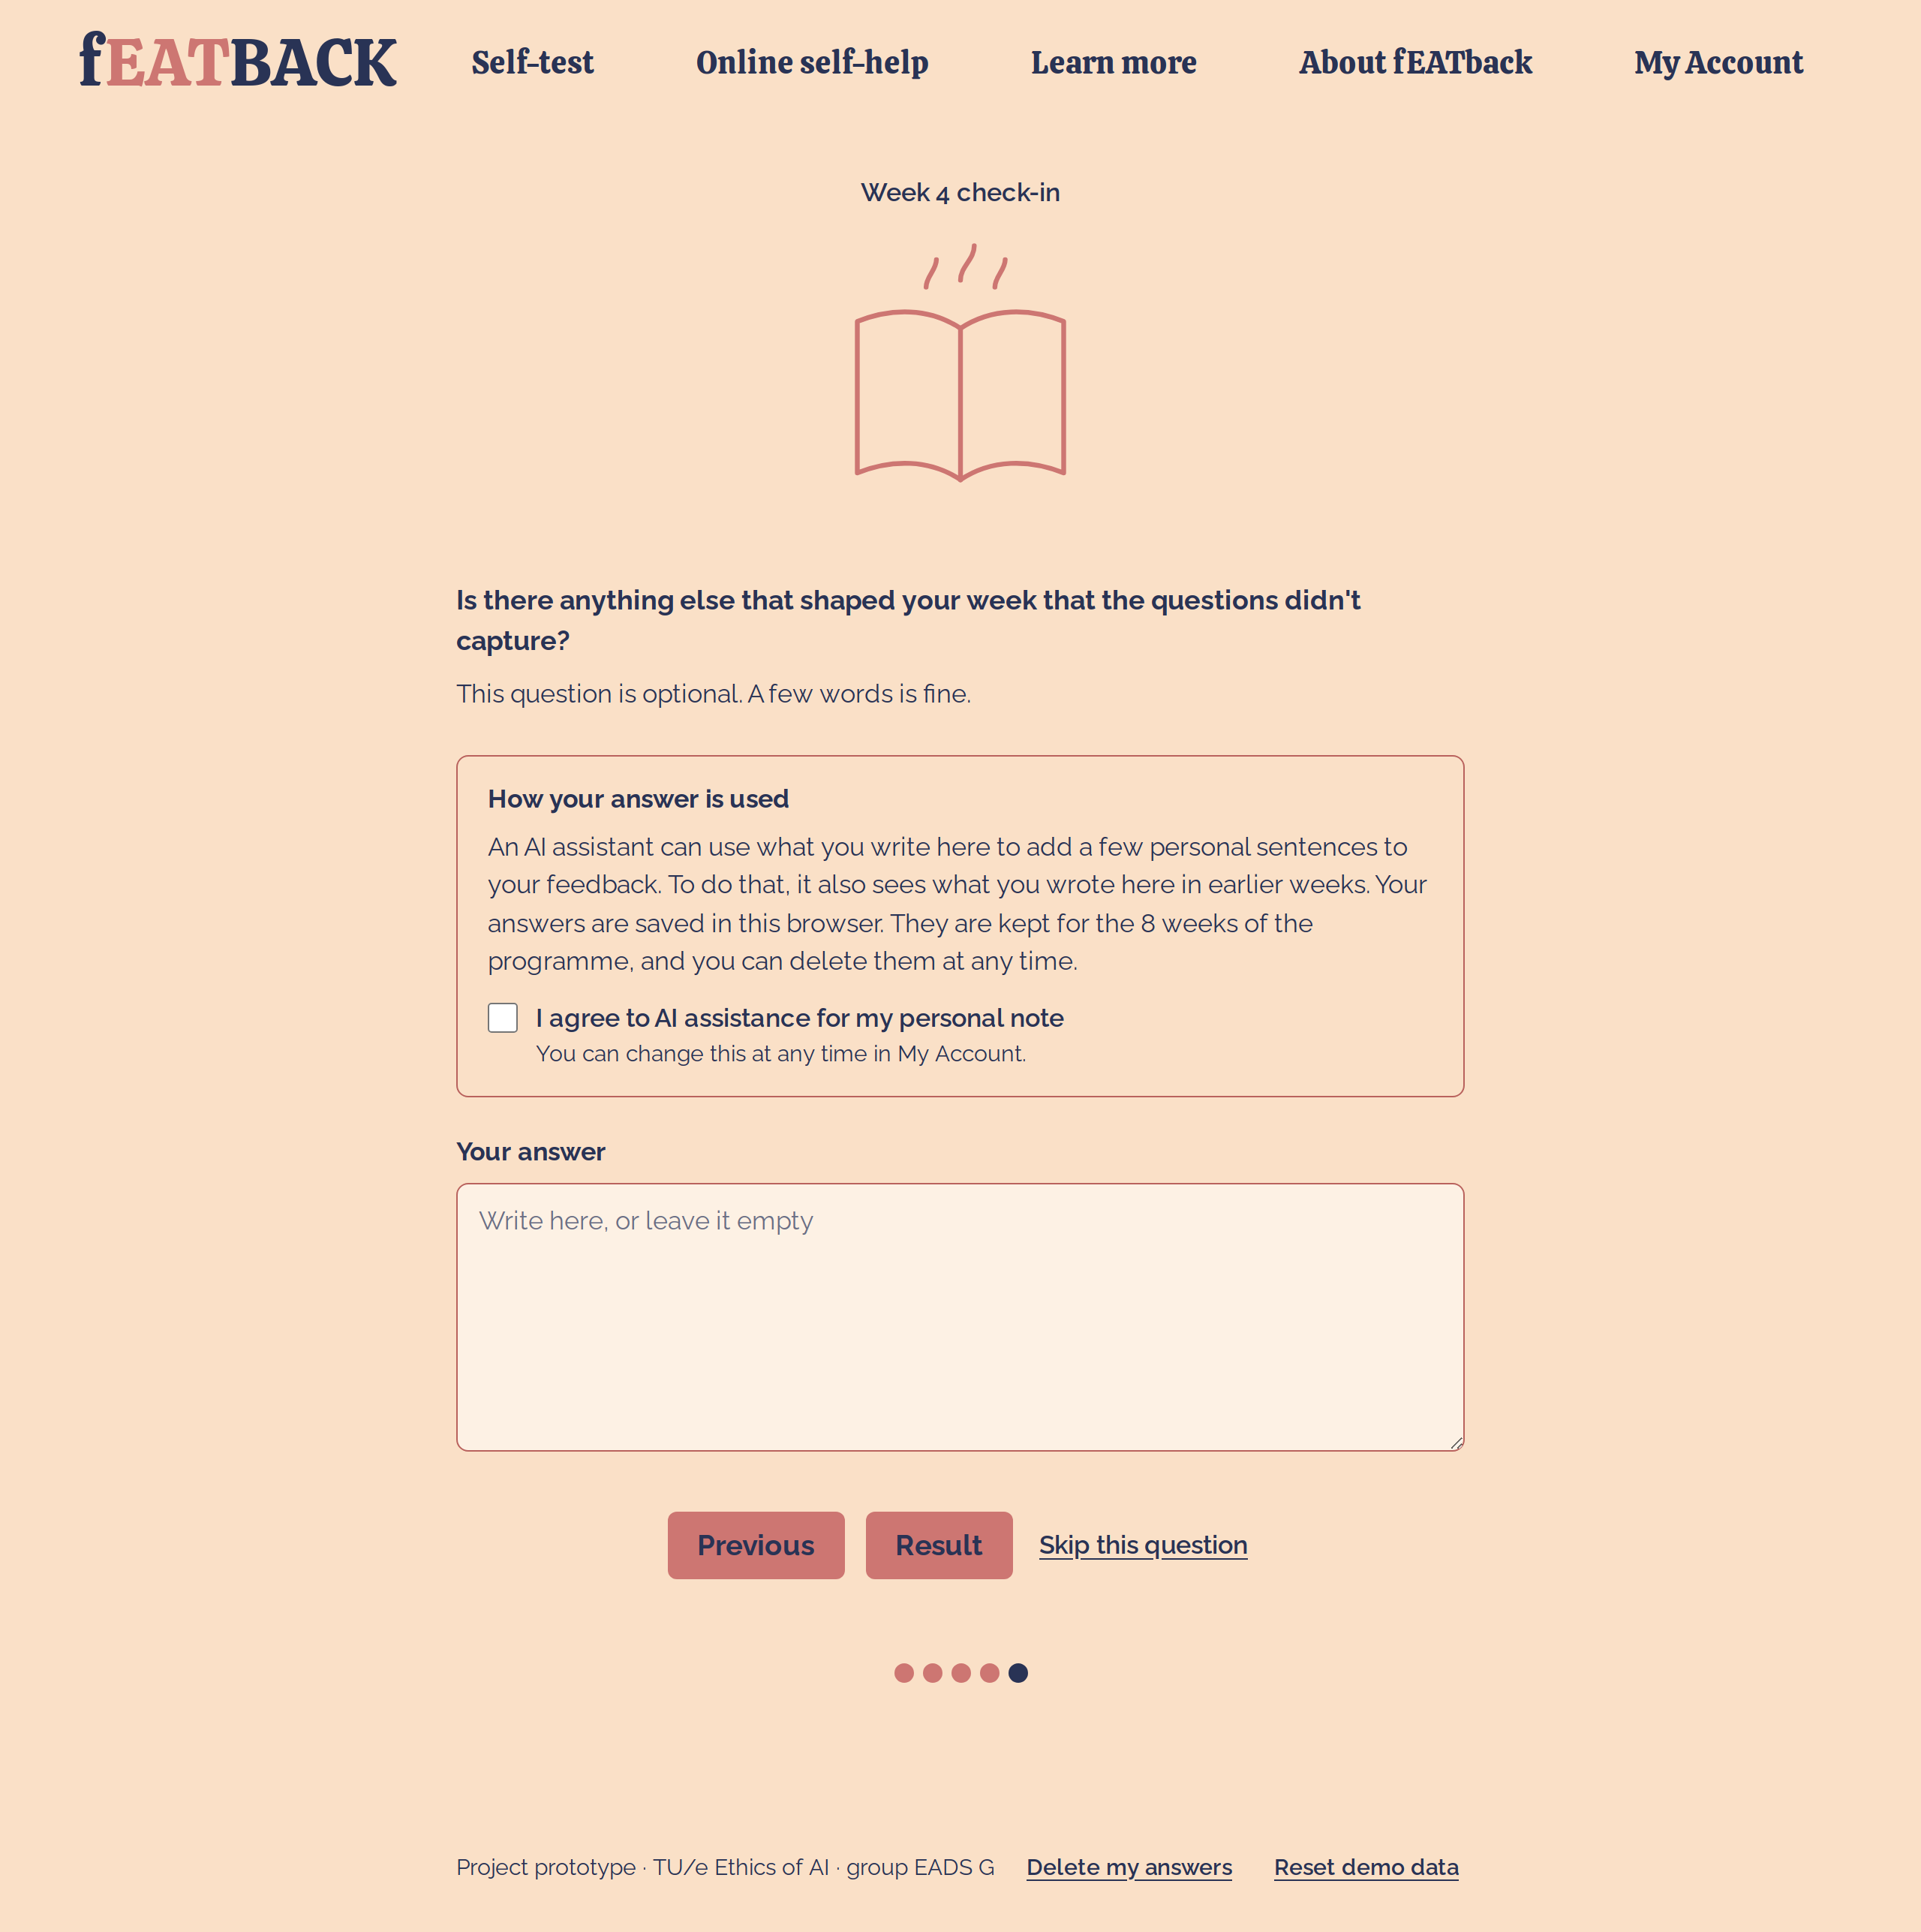
\includegraphics[width=\linewidth, trim=590 1085 590 760, clip]{q5_unticked_v2.png}};
  \begin{scope}[x={(s.south east)}, y={(s.north west)}]
    \callout{0.979}{0.663}{1}
  \end{scope}
\end{tikzpicture}
\par\vspace{4mm}
\paneltitle{b}{Her answer and the full result}
\begin{tikzpicture}
  \node[shot] (s) at (0,0) {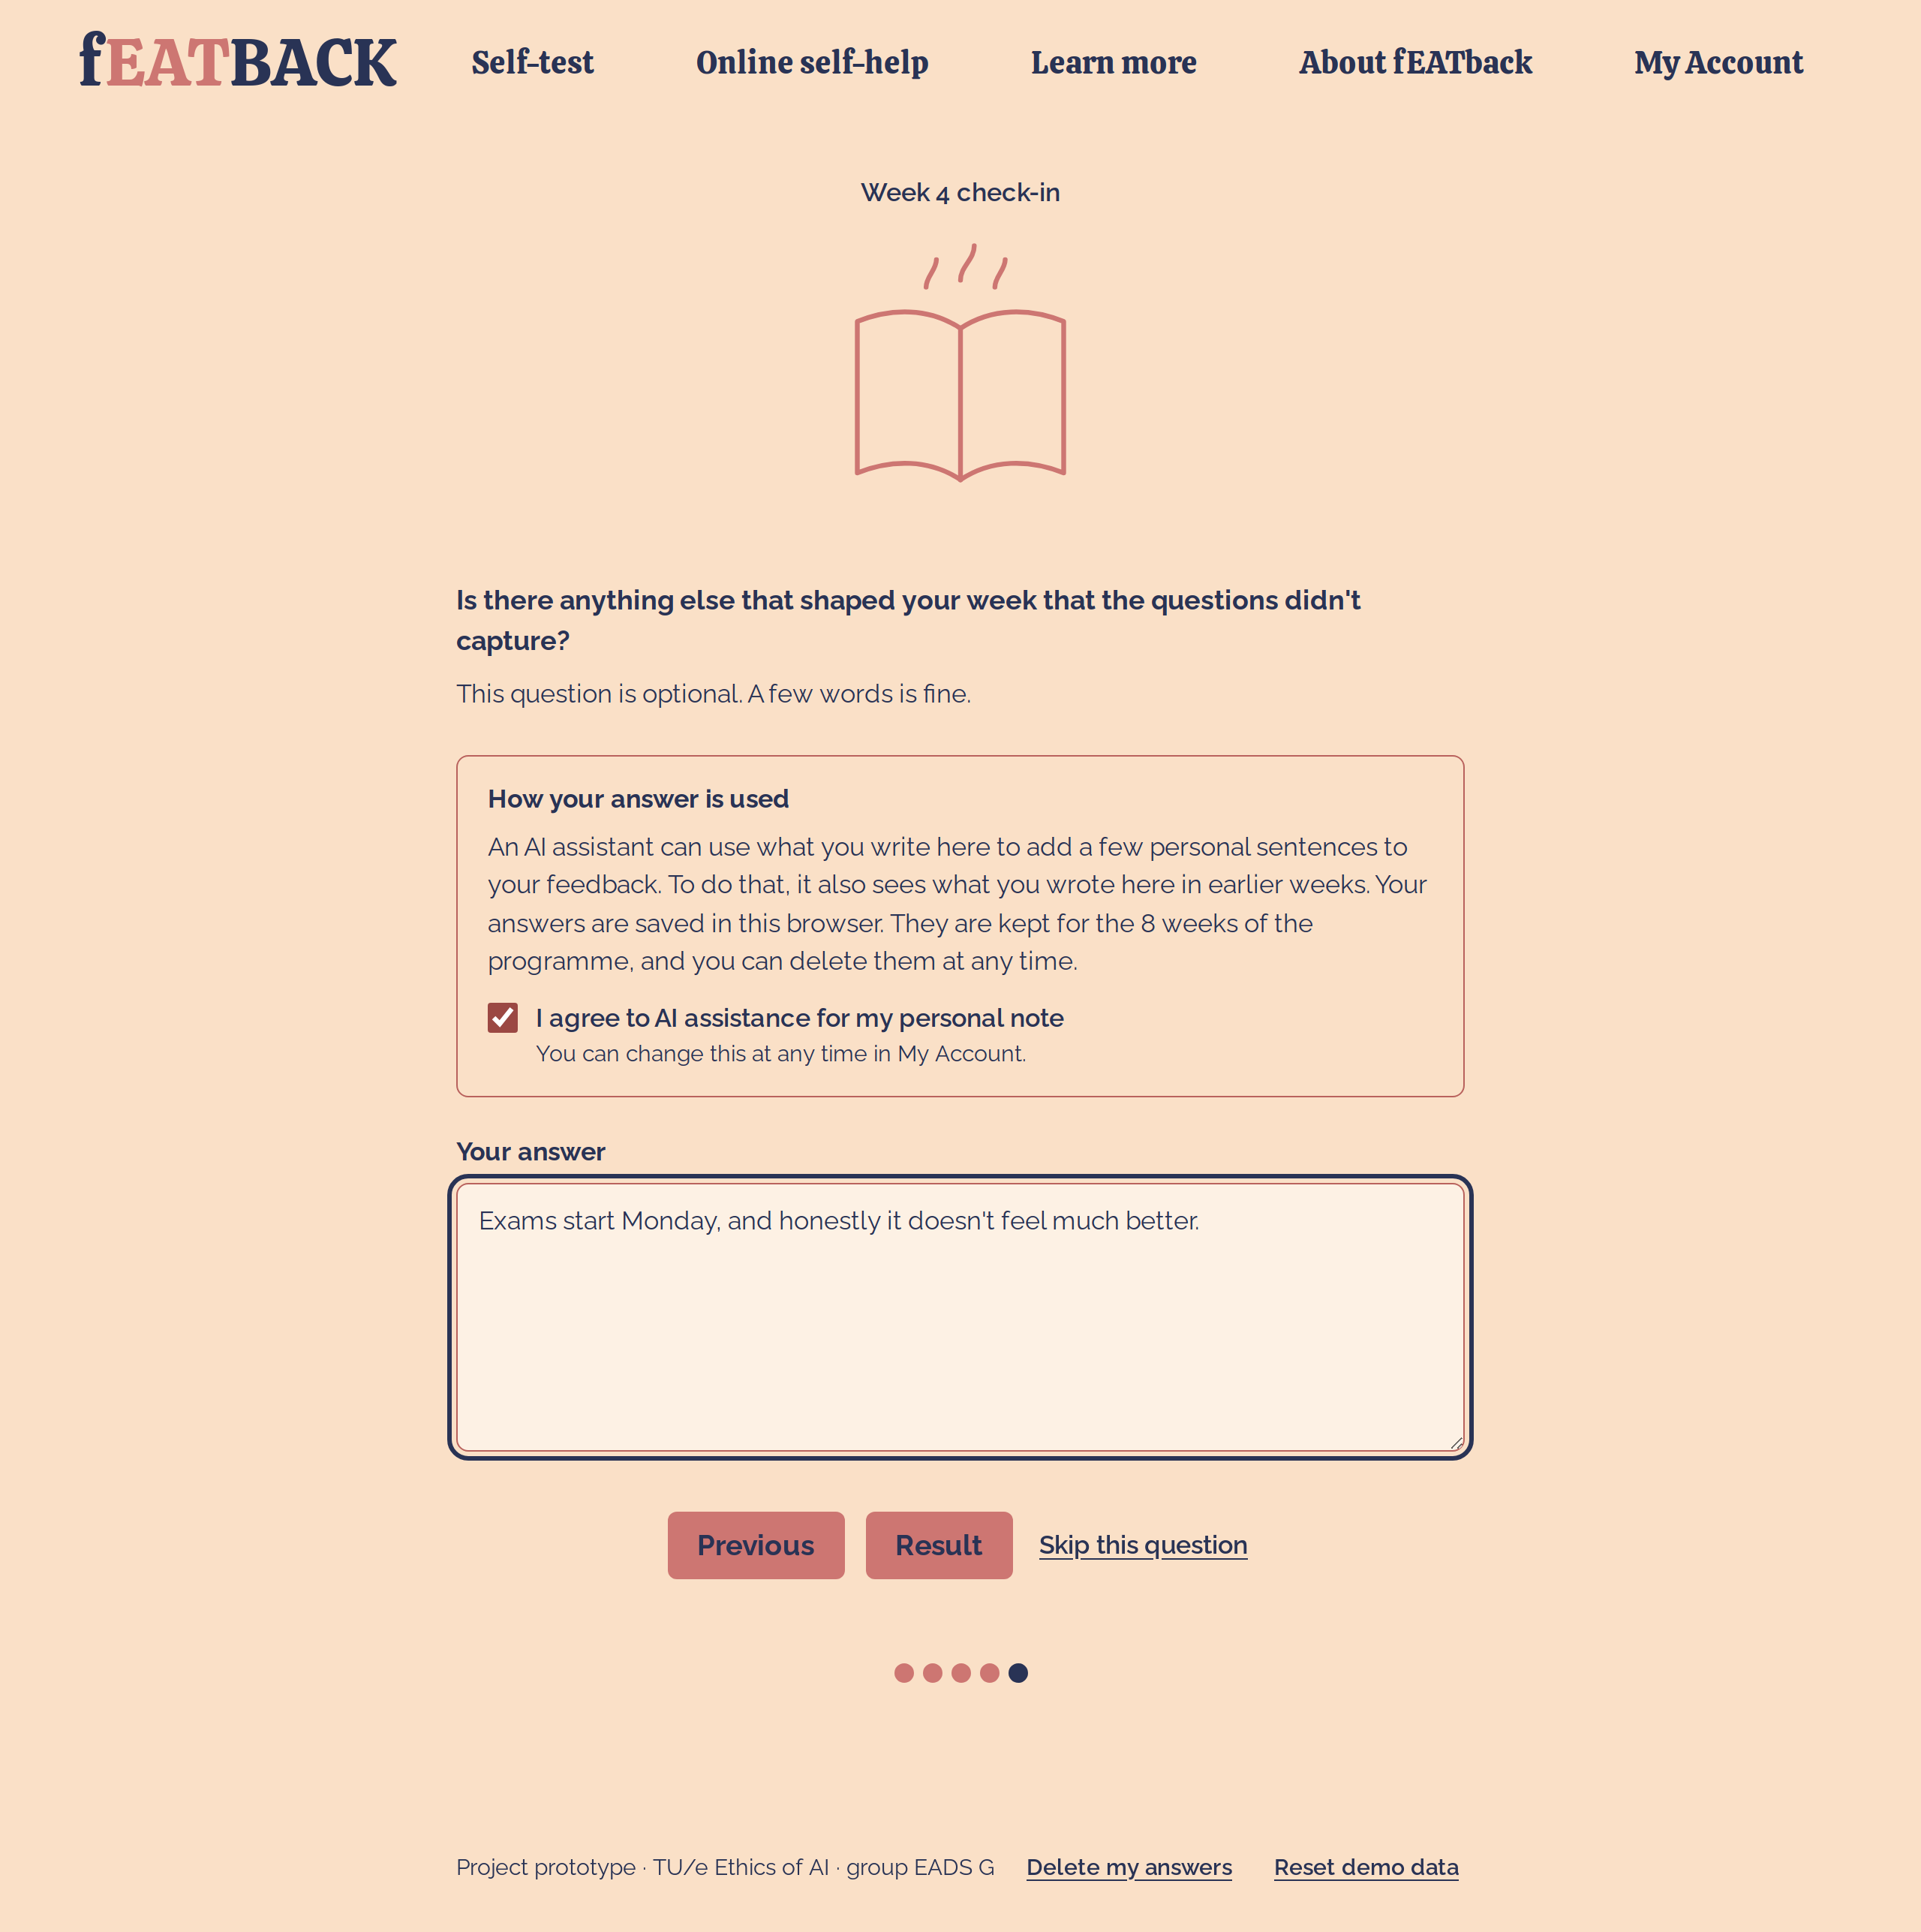
\includegraphics[width=\linewidth, trim=590 613 590 1500, clip]{q5_screen_v2.png}};
  \begin{scope}[x={(s.south east)}, y={(s.north west)}]
    \callout{0.979}{0.835}{2}
  \end{scope}
\end{tikzpicture}
\par\vspace{1.5mm}
\begin{tikzpicture}
  \node[shot] (s) at (0,0) {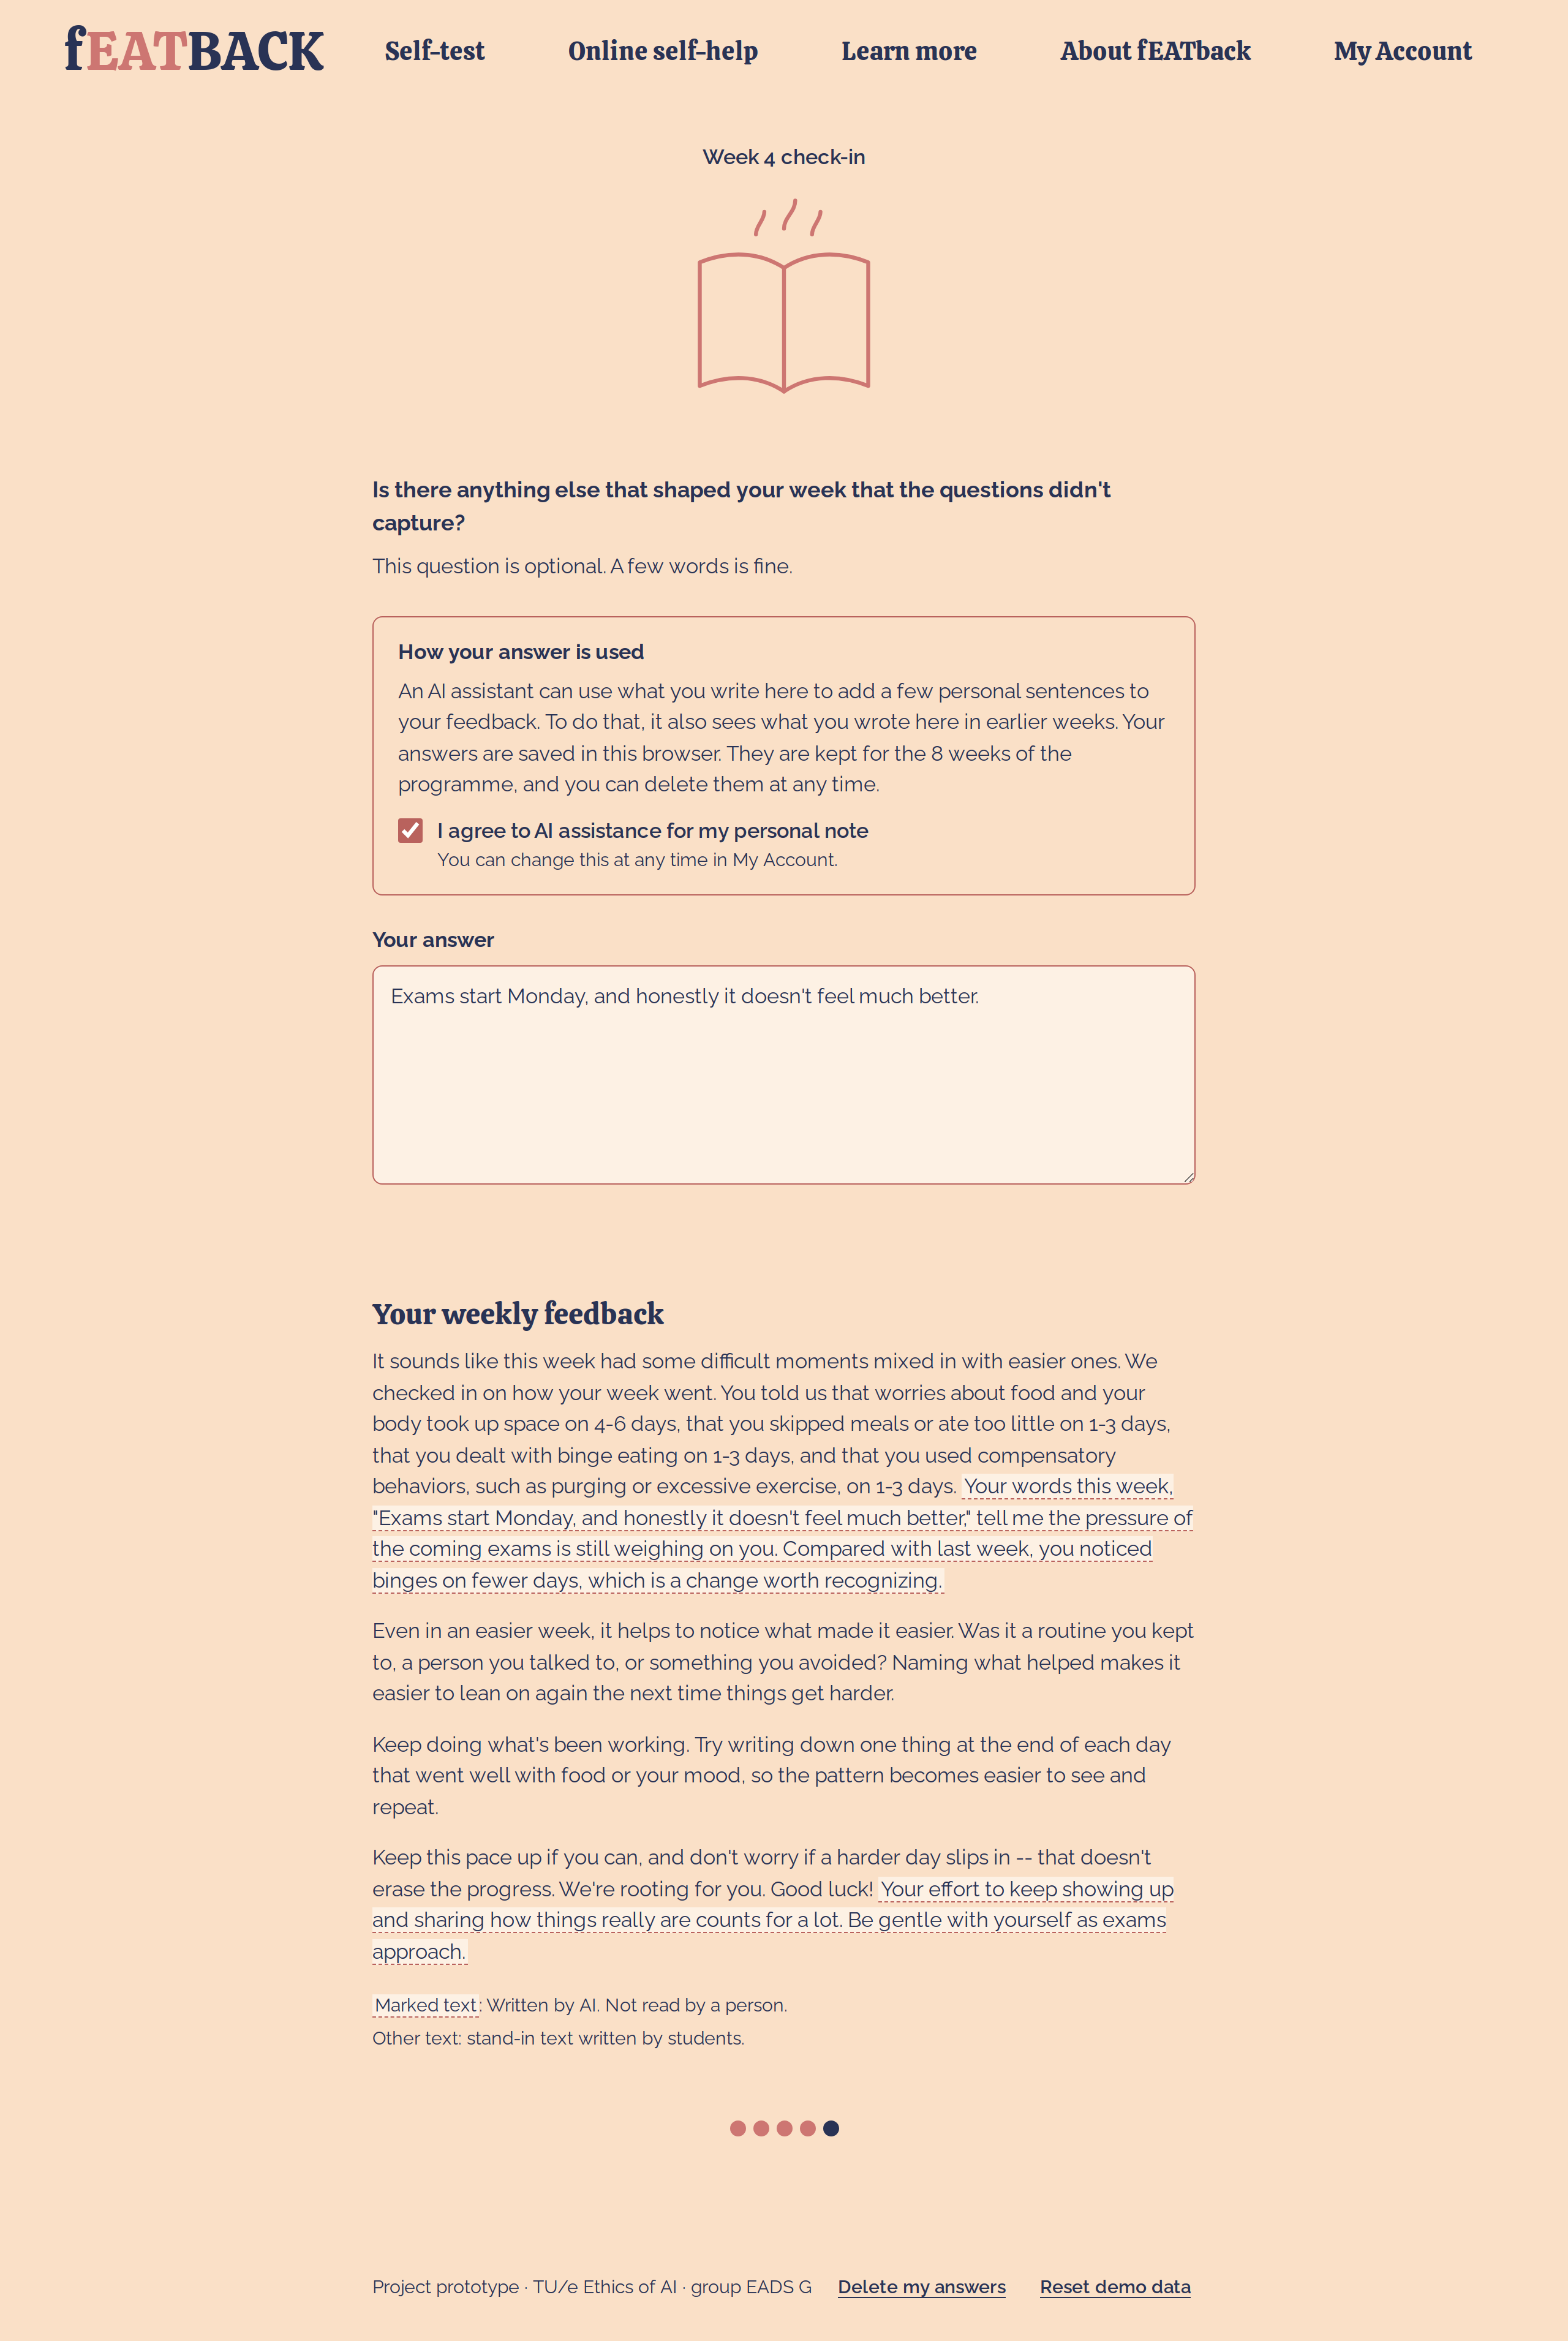
\includegraphics[width=\linewidth, trim=590 451 590 2095, clip]{result_screen_v2.png}};
  \begin{scope}[x={(s.south east)}, y={(s.north west)}]
    \callout{0.979}{0.969}{3}
    \callout{0.979}{0.074}{4}
  \end{scope}
\end{tikzpicture}
\end{minipage}%
\hfill
% ============ Right column: week 5 and the safety paths ============
\begin{minipage}[t]{0.47\textwidth}
\colhead{Week 5 and when something goes wrong}
\paneltitle{c}{Week 5, where the AI text looks back}
\begin{tikzpicture}
  \node[shot] (s) at (0,0) {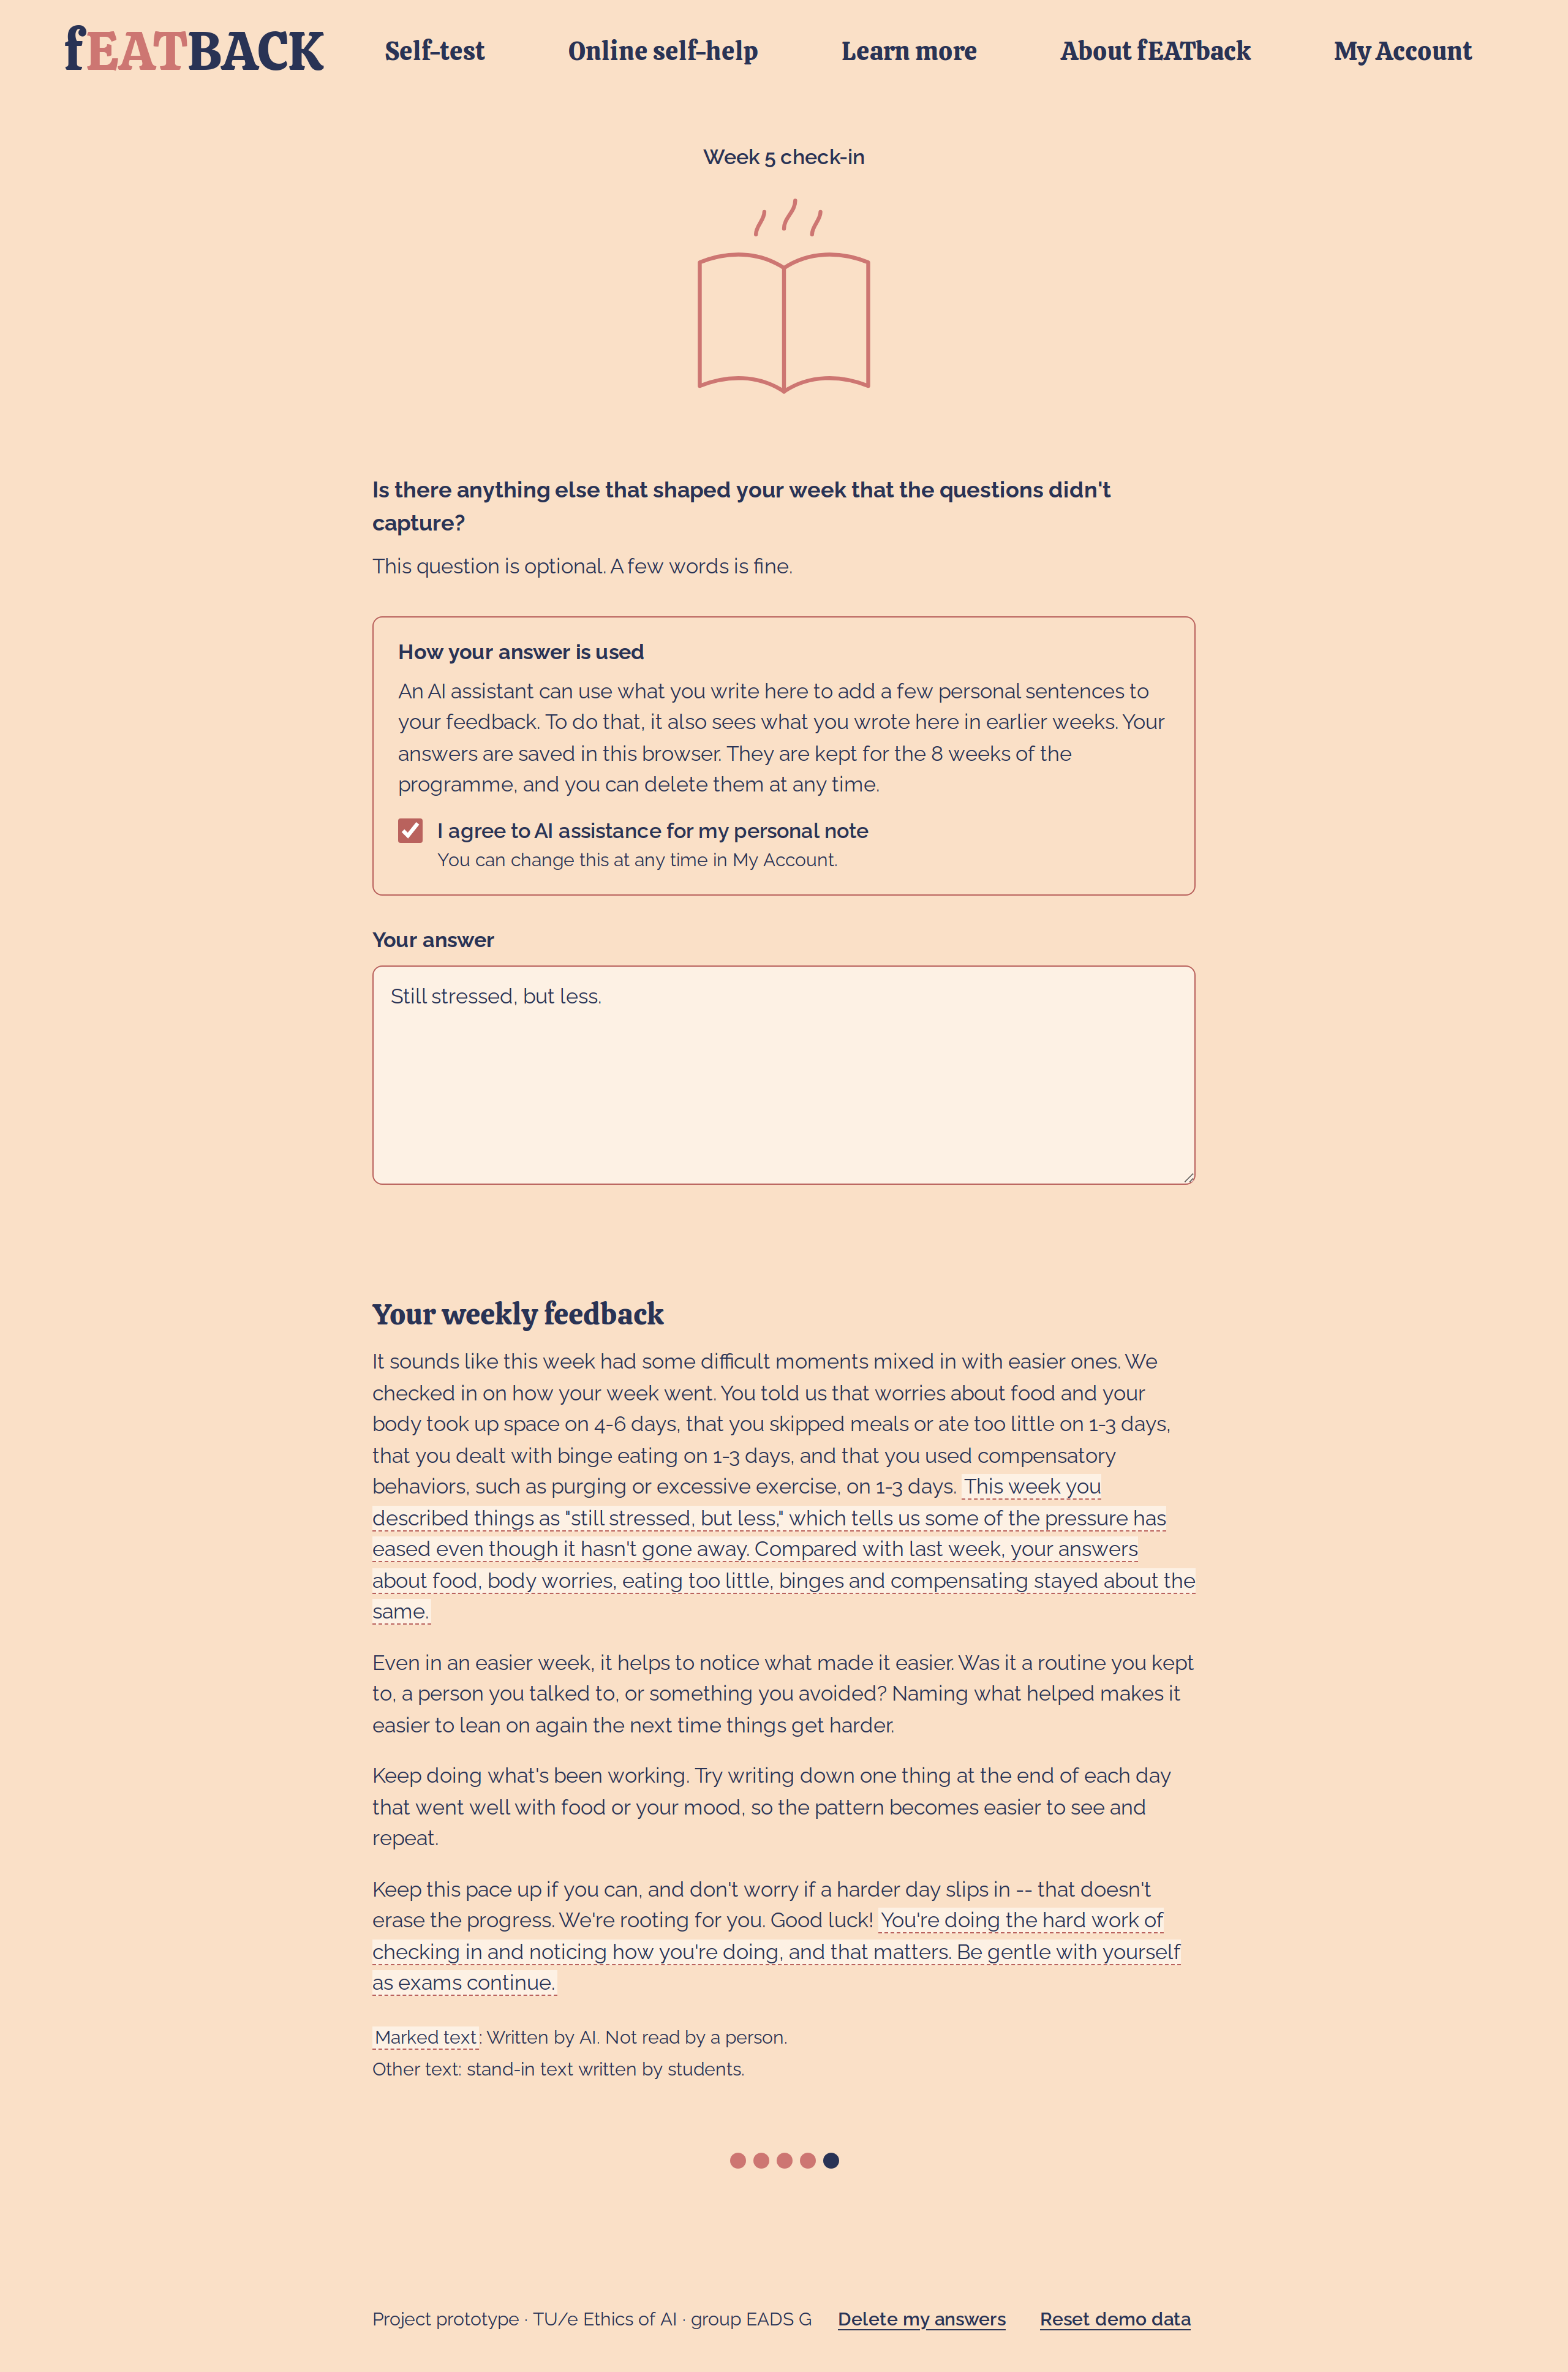
\includegraphics[width=\linewidth, trim=590 1911 590 1500, clip]{result_week5_v2.png}};
\end{tikzpicture}
\par\vspace{1.5mm}
\begin{tikzpicture}
  \node[shot] (s) at (0,0) {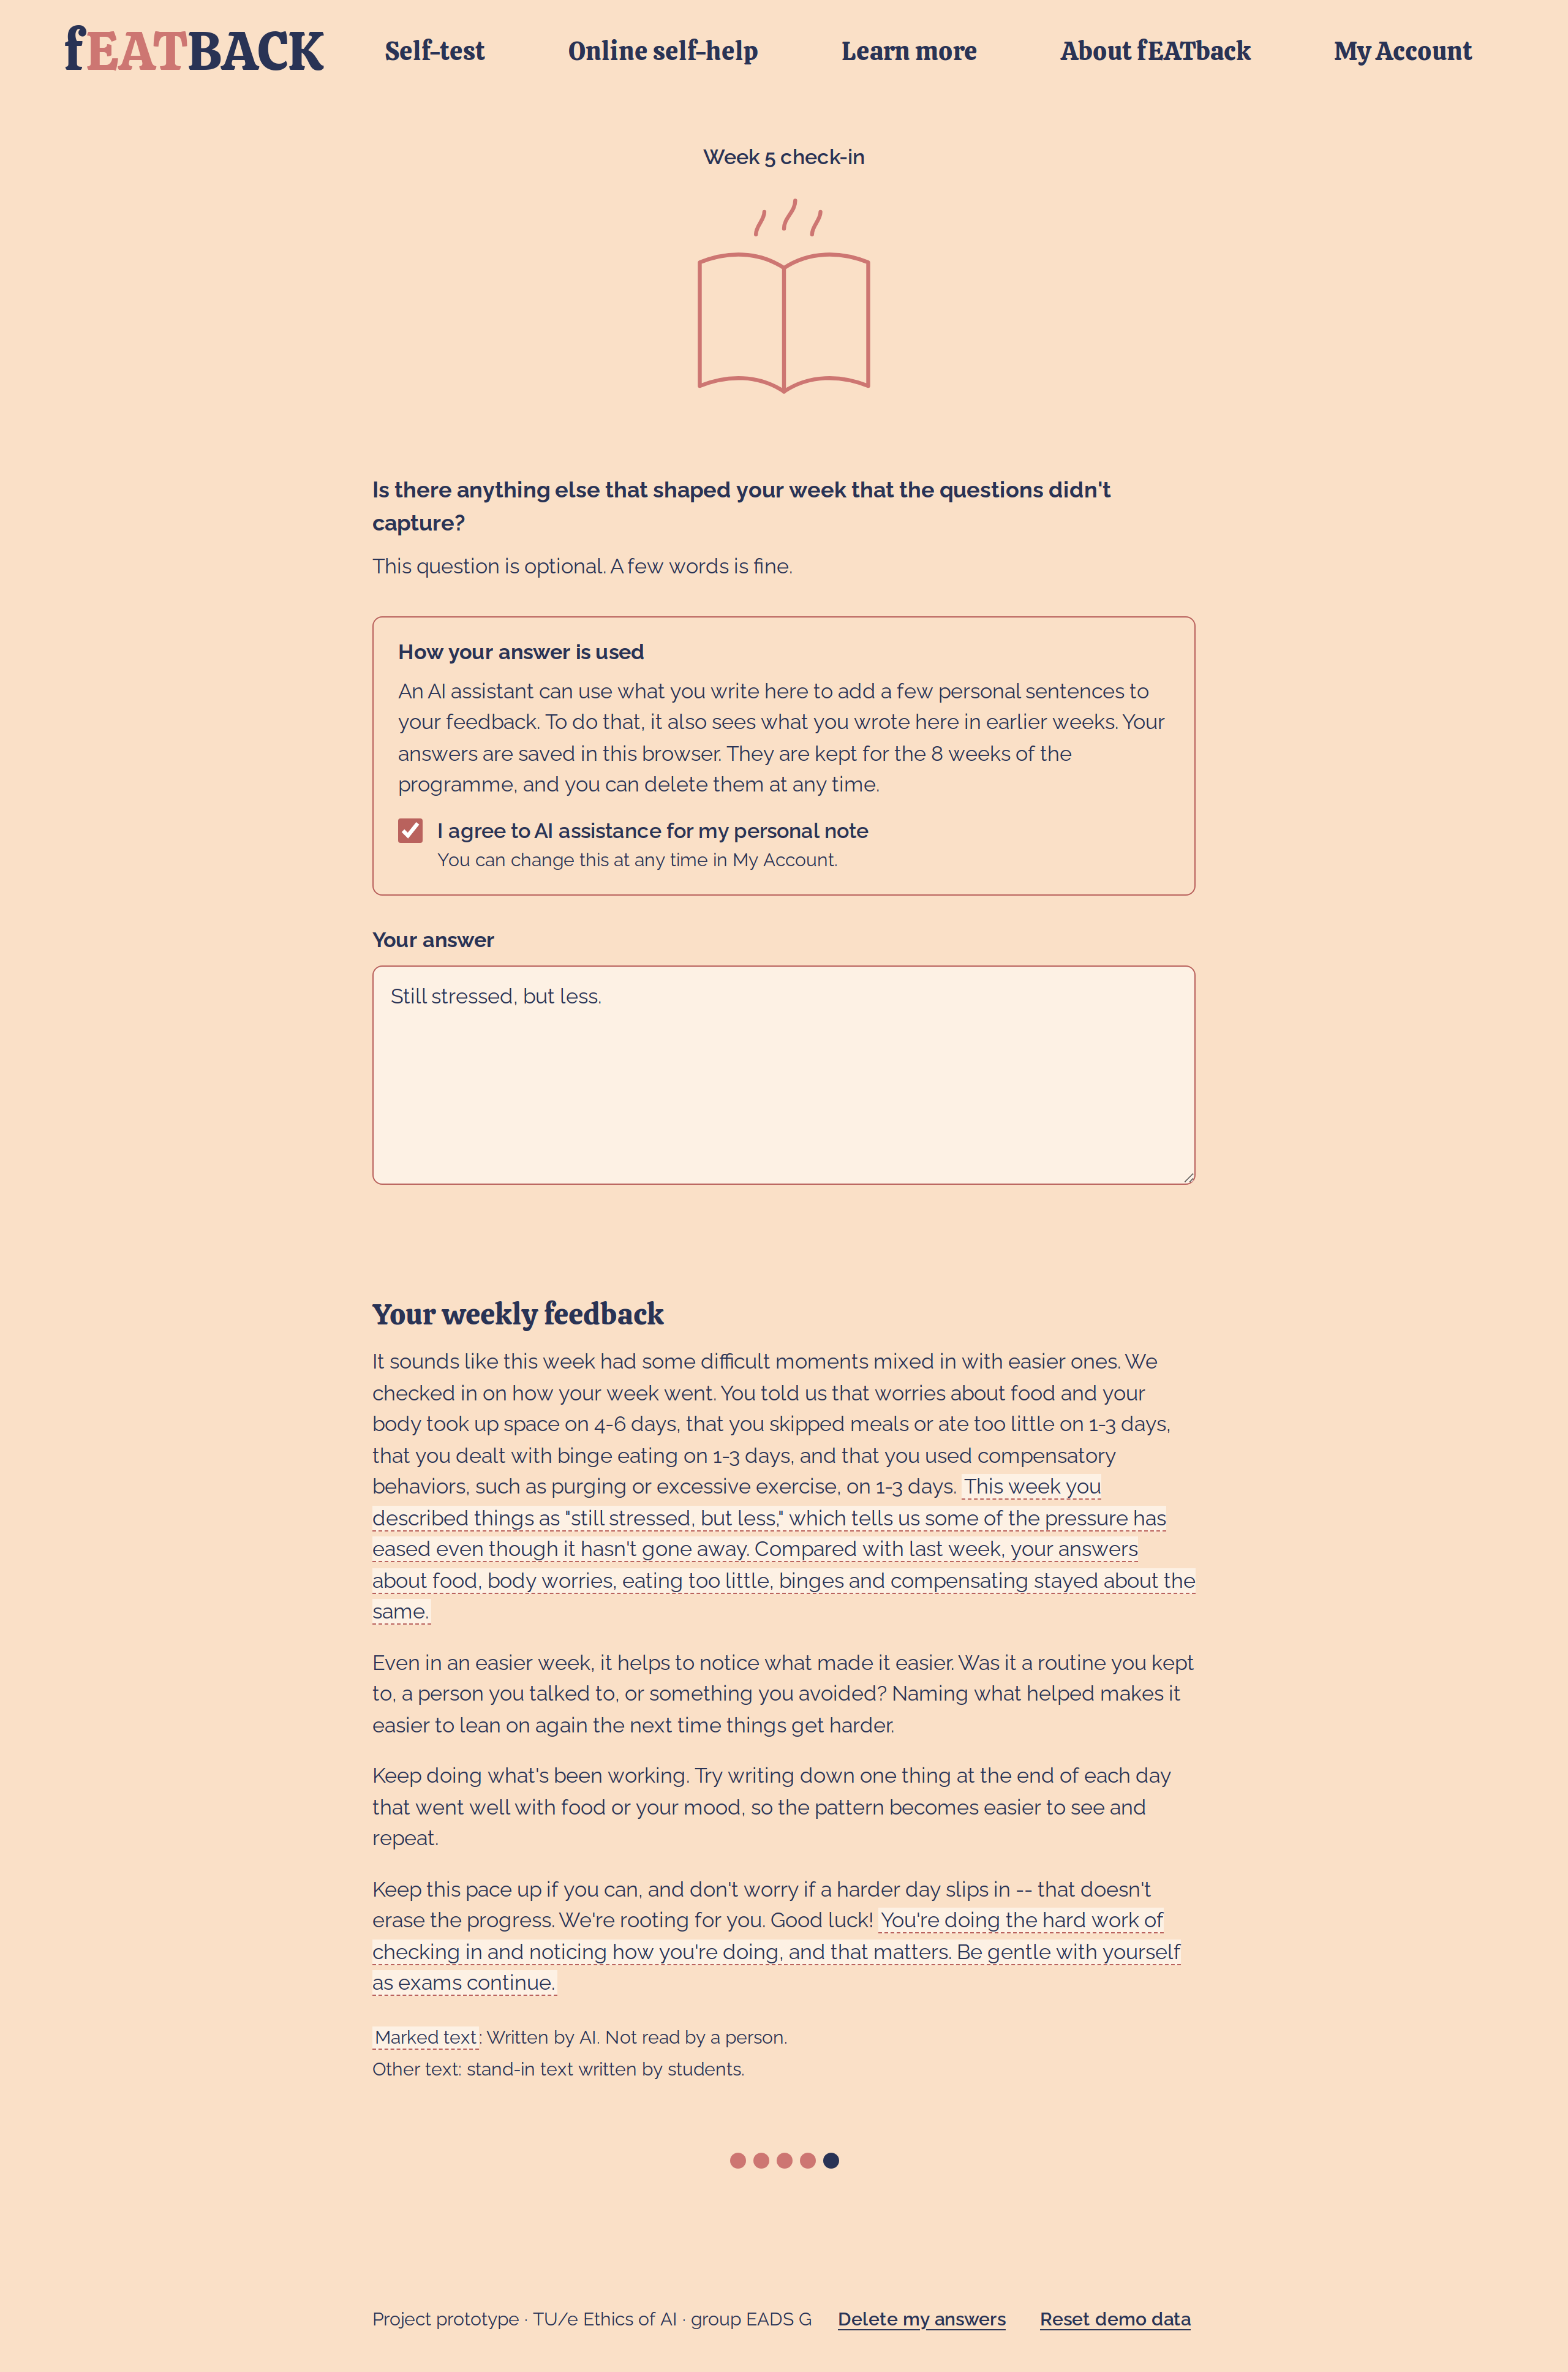
\includegraphics[width=\linewidth, trim=590 1203 590 2095, clip]{result_week5_v2.png}};
\end{tikzpicture}
\par\vspace{4mm}
\paneltitle{d}{Model off or AI text rejected}
\begin{tikzpicture}
  \node[shot] (s) at (0,0) {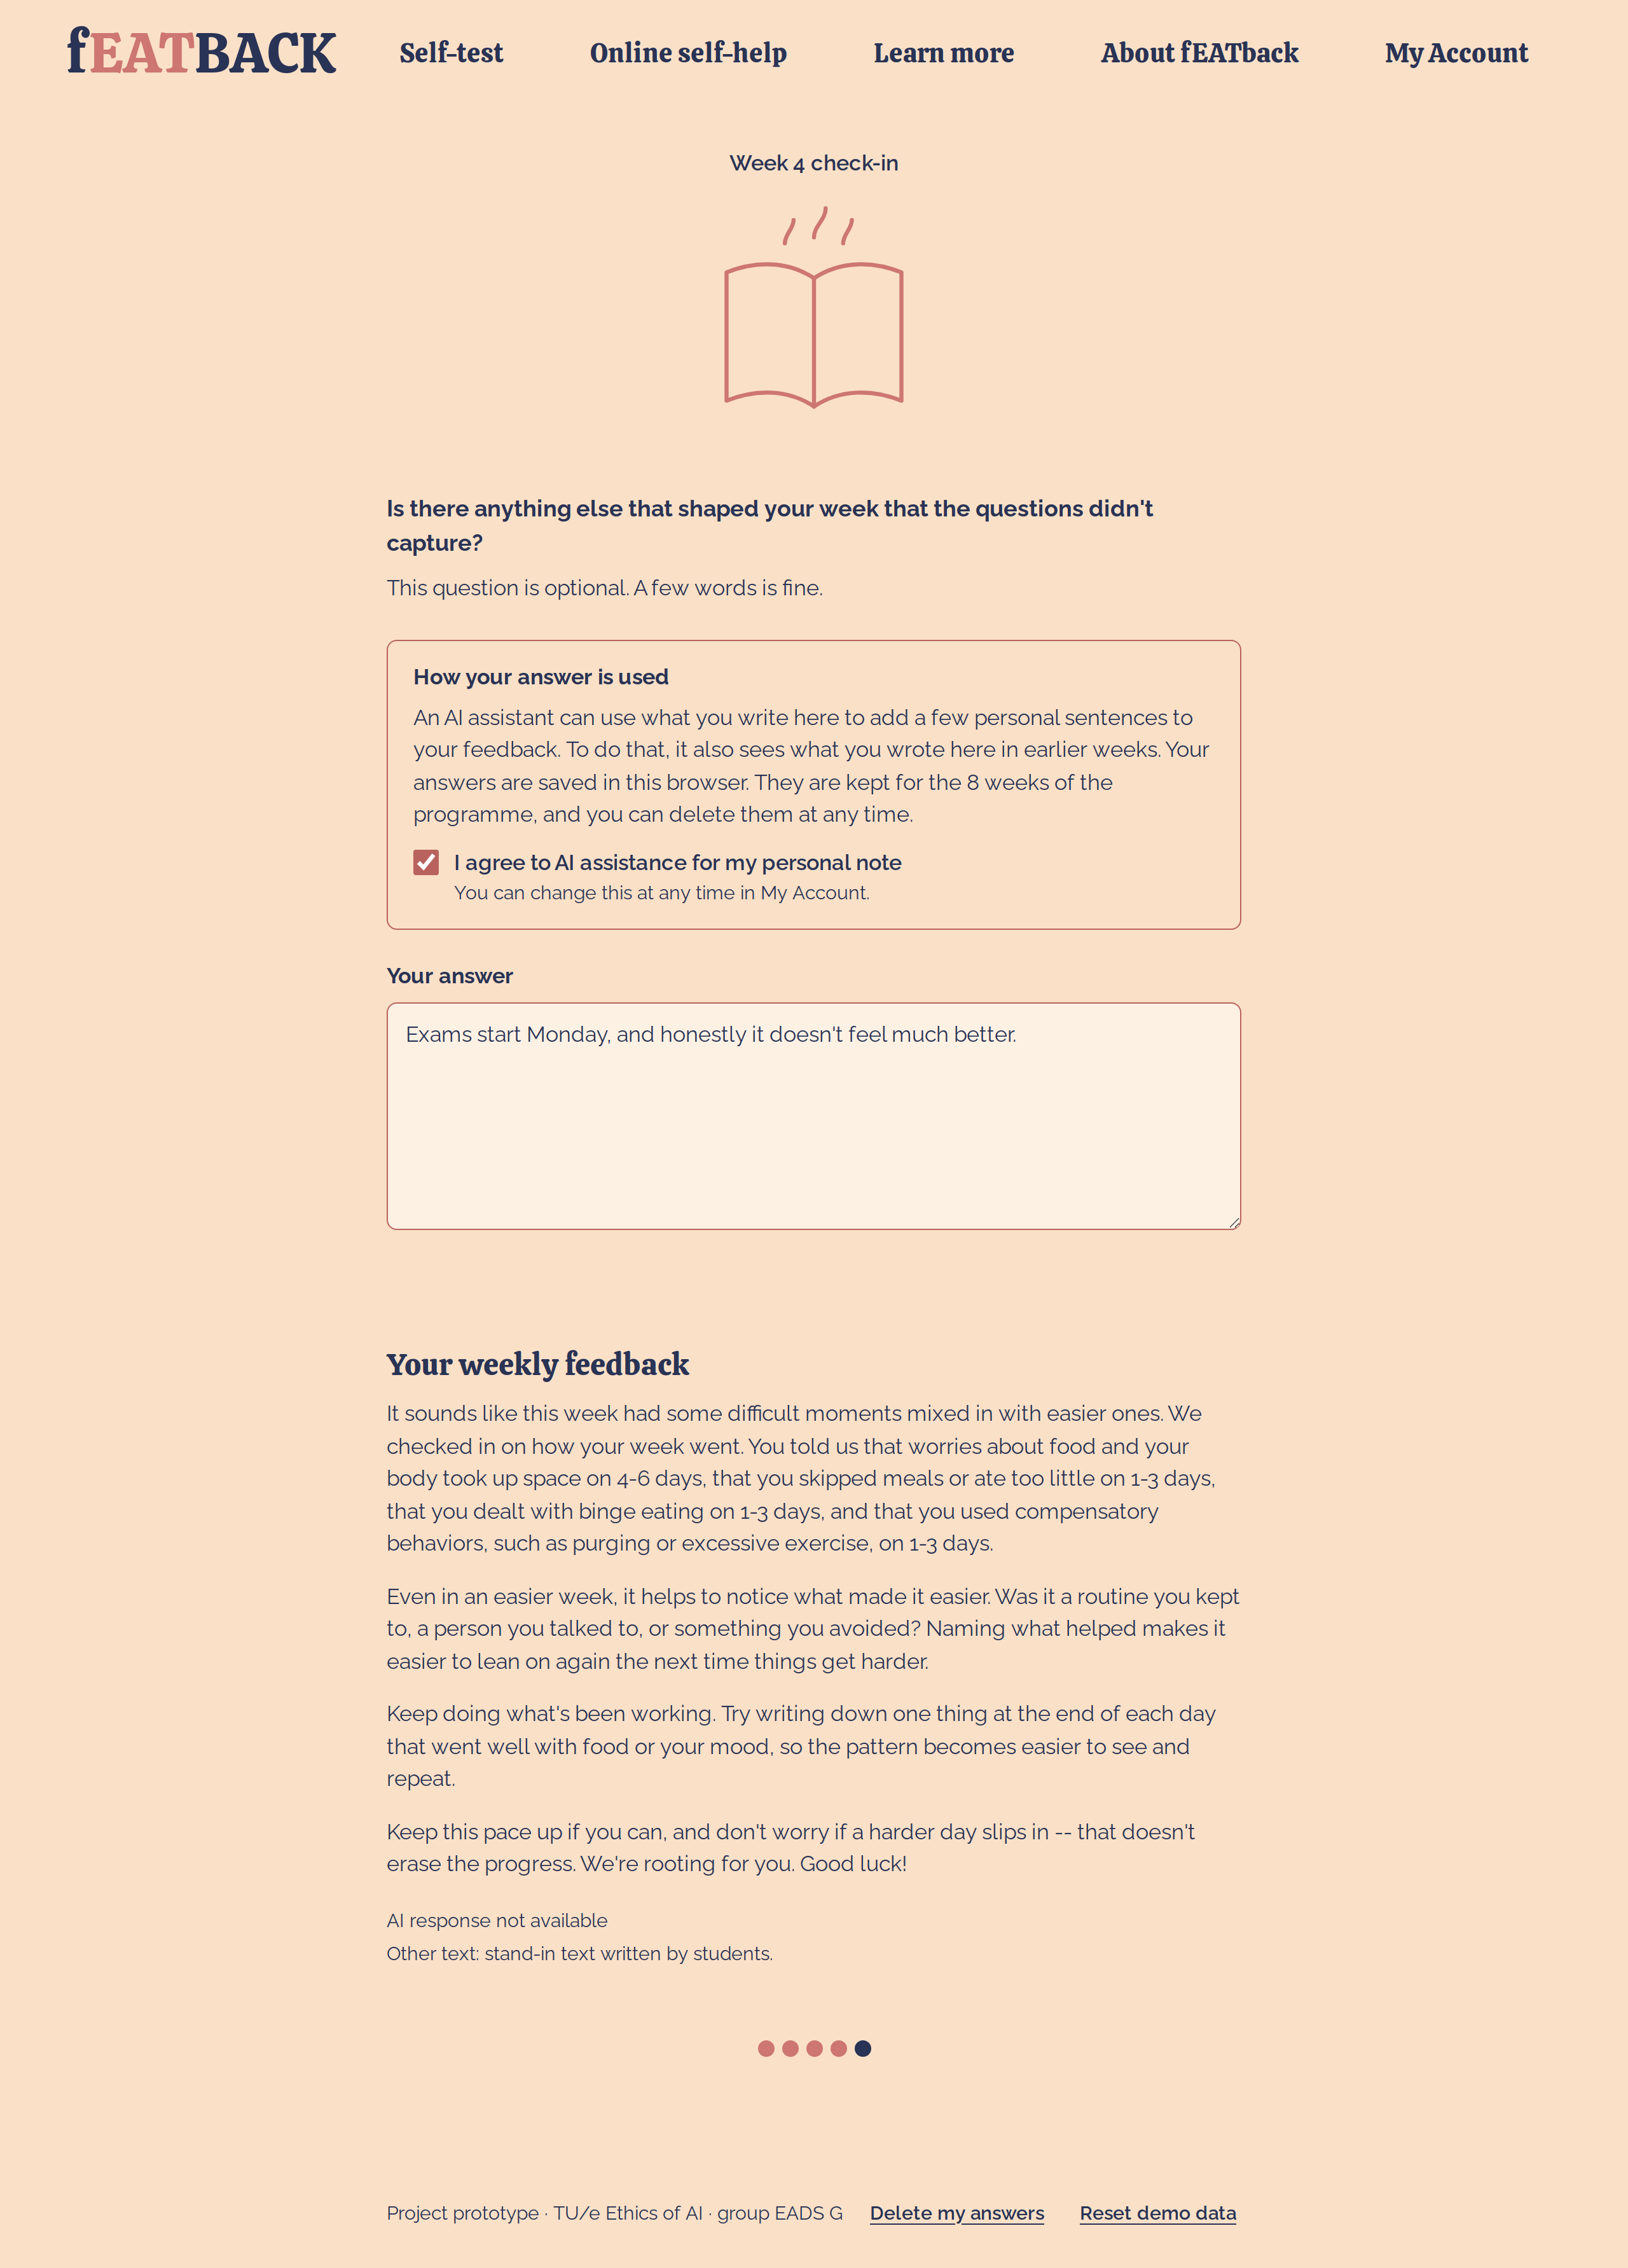
\includegraphics[width=\linewidth, trim=590 451 590 2850, clip]{fallback_v2.png}};
  \begin{scope}[x={(s.south east)}, y={(s.north west)}]
    \callout{0.979}{0.355}{5}
  \end{scope}
\end{tikzpicture}
\par\vspace{4mm}
\paneltitle{e}{An answer with signs of acute risk}
\begin{tikzpicture}
  \node[shot] (s) at (0,0) {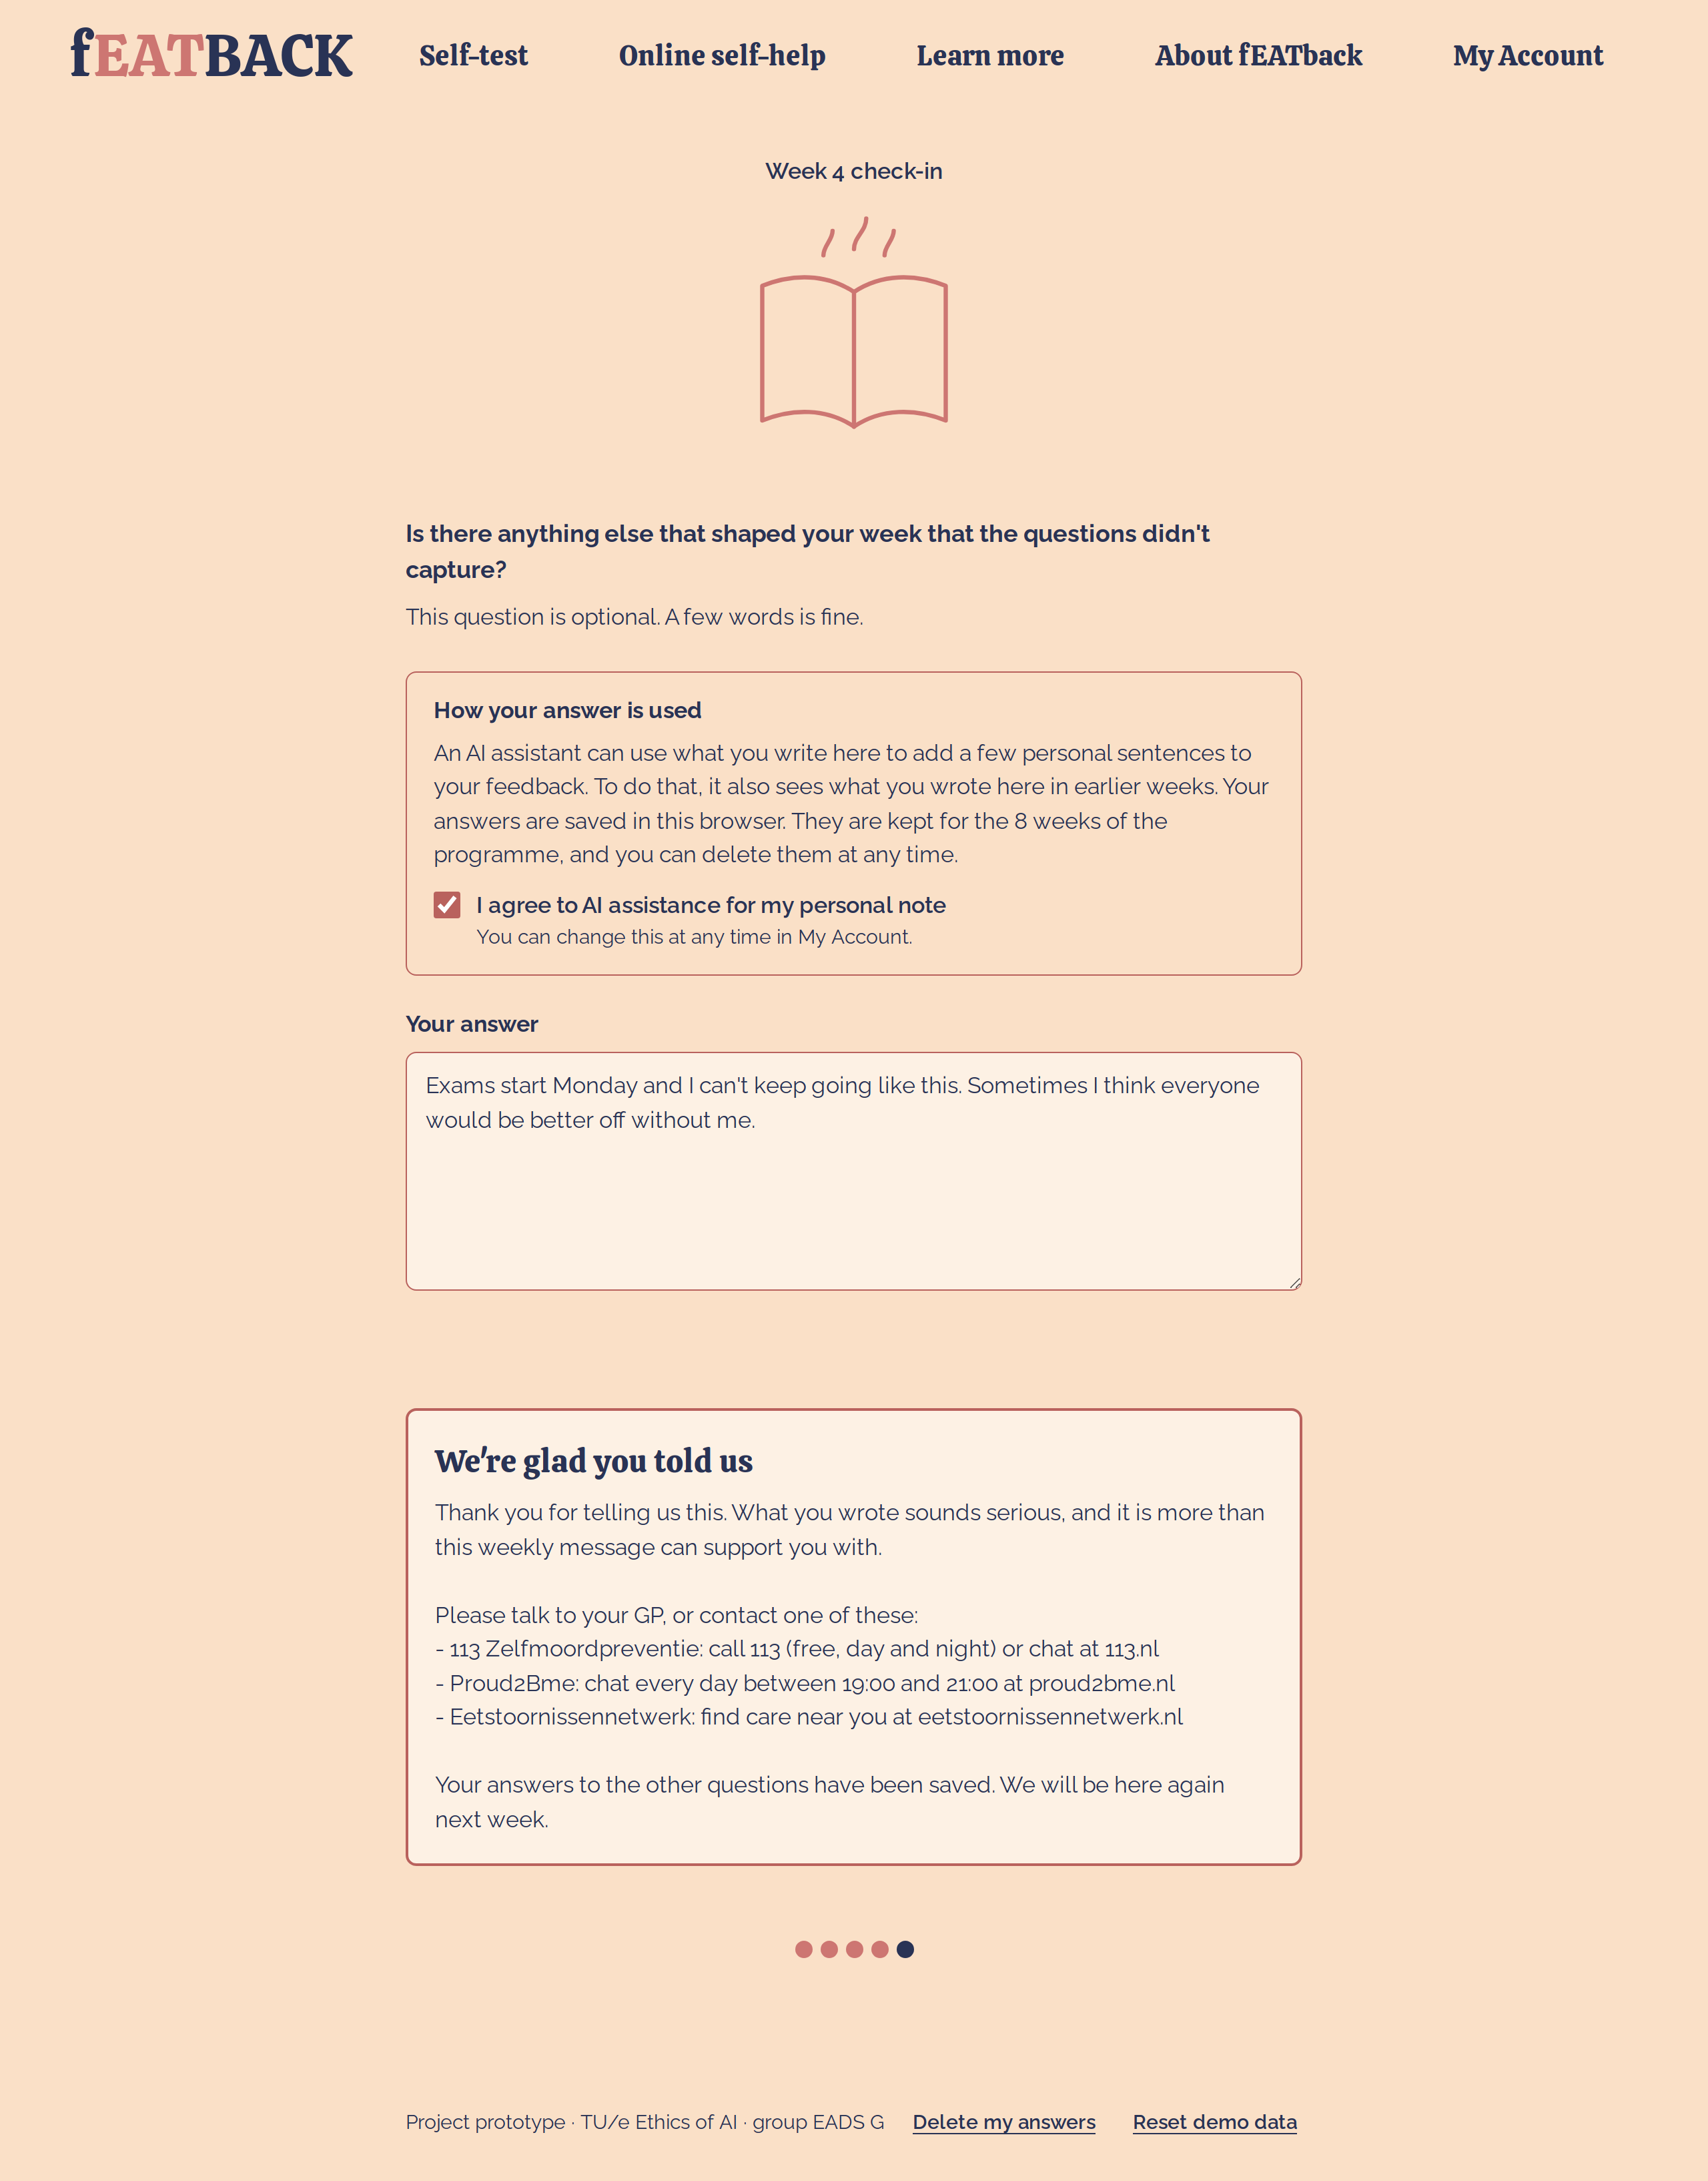
\includegraphics[width=\linewidth, trim=590 1307 590 1500, clip]{acute_v2.png}};
\end{tikzpicture}
\par\vspace{1.5mm}
\begin{tikzpicture}
  \node[shot] (s) at (0,0) {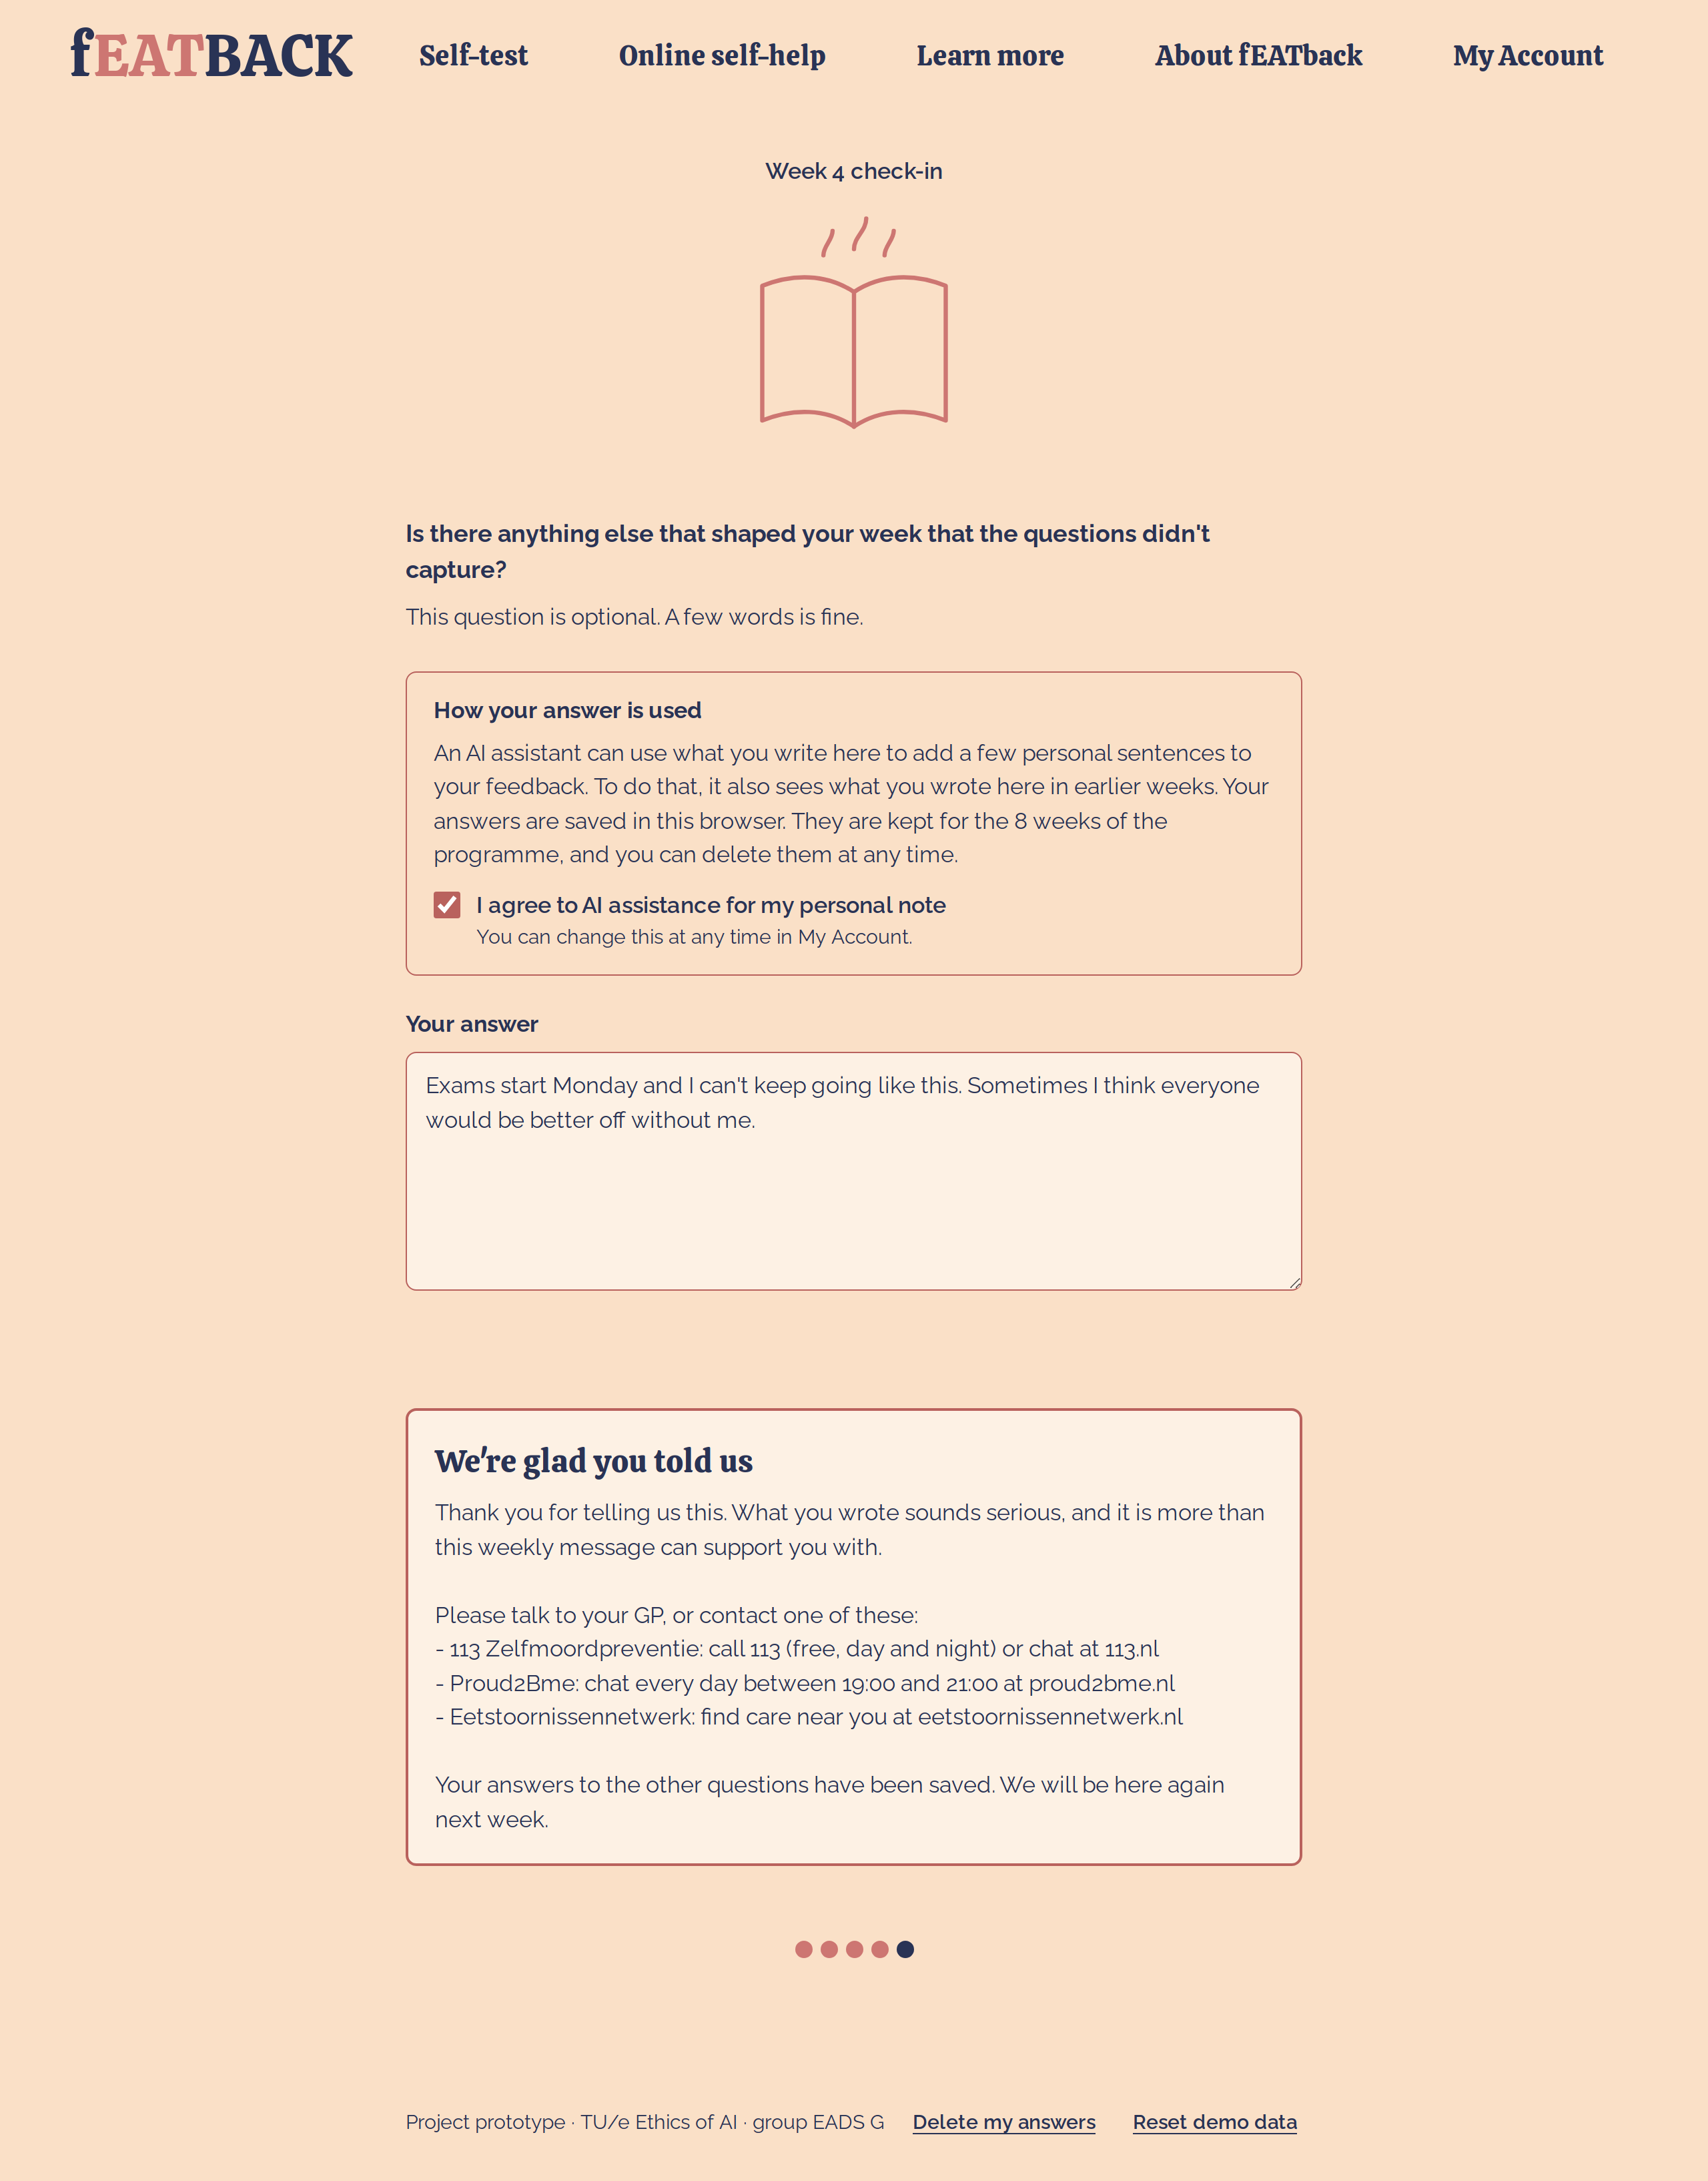
\includegraphics[width=\linewidth, trim=590 445 590 2082, clip]{acute_v2.png}};
  \begin{scope}[x={(s.south east)}, y={(s.north west)}]
    \callout{0.979}{0.962}{6}
  \end{scope}
\end{tikzpicture}
\end{minipage}

\vspace{5mm}
% ---- Key: one entry per callout, aligned with the two columns ----
\newcommand{\keyline}[2]{\key{#1}\hspace{2mm}#2\par\vspace{1.2mm}}
{\footnotesize\sffamily
\begin{minipage}[t]{0.47\textwidth}
\keyline{1}{Consent box starts unticked (part 3)}
\keyline{2}{Answer stored for the trend (part 3)}
\keyline{3}{Unmarked text: stand-in bank message (part 1)}
\end{minipage}\hfill
\begin{minipage}[t]{0.47\textwidth}
\keyline{4}{AI text is marked and labelled (part 2)}
\keyline{5}{Fallback: the bank's own text only (part 1)}
\keyline{6}{Gate takes the more severe label (part 1)}
\end{minipage}}

\vspace{2mm}
\caption{Maren's check-ins from Section~\ref{sec:narrative} as they appear on screen. Part numbers in the key
point to the Responsible Innovation statement. The marked text in (b) and (c) is real
output from our fine-tuned writer model, run on 12 October 2026. The bank message, Maren
and her earlier answers are made up for the demo.}
\label{fig:mockup}
\end{figure}
